\documentclass[]{article}
\usepackage{lmodern}
\usepackage{amssymb,amsmath}
\usepackage{ifxetex,ifluatex}
\usepackage{fixltx2e} % provides \textsubscript
\ifnum 0\ifxetex 1\fi\ifluatex 1\fi=0 % if pdftex
  \usepackage[T1]{fontenc}
  \usepackage[utf8]{inputenc}
\else % if luatex or xelatex
  \ifxetex
    \usepackage{mathspec}
    \usepackage{xltxtra,xunicode}
  \else
    \usepackage{fontspec}
  \fi
  \defaultfontfeatures{Mapping=tex-text,Scale=MatchLowercase}
  \newcommand{\euro}{€}
\fi
% use upquote if available, for straight quotes in verbatim environments
\IfFileExists{upquote.sty}{\usepackage{upquote}}{}
% use microtype if available
\IfFileExists{microtype.sty}{%
\usepackage{microtype}
\UseMicrotypeSet[protrusion]{basicmath} % disable protrusion for tt fonts
}{}
\usepackage[margin=1in]{geometry}
\usepackage{color}
\usepackage{fancyvrb}
\newcommand{\VerbBar}{|}
\newcommand{\VERB}{\Verb[commandchars=\\\{\}]}
\DefineVerbatimEnvironment{Highlighting}{Verbatim}{commandchars=\\\{\}}
% Add ',fontsize=\small' for more characters per line
\usepackage{framed}
\definecolor{shadecolor}{RGB}{248,248,248}
\newenvironment{Shaded}{\begin{snugshade}}{\end{snugshade}}
\newcommand{\KeywordTok}[1]{\textcolor[rgb]{0.13,0.29,0.53}{\textbf{{#1}}}}
\newcommand{\DataTypeTok}[1]{\textcolor[rgb]{0.13,0.29,0.53}{{#1}}}
\newcommand{\DecValTok}[1]{\textcolor[rgb]{0.00,0.00,0.81}{{#1}}}
\newcommand{\BaseNTok}[1]{\textcolor[rgb]{0.00,0.00,0.81}{{#1}}}
\newcommand{\FloatTok}[1]{\textcolor[rgb]{0.00,0.00,0.81}{{#1}}}
\newcommand{\CharTok}[1]{\textcolor[rgb]{0.31,0.60,0.02}{{#1}}}
\newcommand{\StringTok}[1]{\textcolor[rgb]{0.31,0.60,0.02}{{#1}}}
\newcommand{\CommentTok}[1]{\textcolor[rgb]{0.56,0.35,0.01}{\textit{{#1}}}}
\newcommand{\OtherTok}[1]{\textcolor[rgb]{0.56,0.35,0.01}{{#1}}}
\newcommand{\AlertTok}[1]{\textcolor[rgb]{0.94,0.16,0.16}{{#1}}}
\newcommand{\FunctionTok}[1]{\textcolor[rgb]{0.00,0.00,0.00}{{#1}}}
\newcommand{\RegionMarkerTok}[1]{{#1}}
\newcommand{\ErrorTok}[1]{\textbf{{#1}}}
\newcommand{\NormalTok}[1]{{#1}}
\usepackage{longtable,booktabs}
\usepackage{graphicx}
\makeatletter
\def\maxwidth{\ifdim\Gin@nat@width>\linewidth\linewidth\else\Gin@nat@width\fi}
\def\maxheight{\ifdim\Gin@nat@height>\textheight\textheight\else\Gin@nat@height\fi}
\makeatother
% Scale images if necessary, so that they will not overflow the page
% margins by default, and it is still possible to overwrite the defaults
% using explicit options in \includegraphics[width, height, ...]{}
\setkeys{Gin}{width=\maxwidth,height=\maxheight,keepaspectratio}
\ifxetex
  \usepackage[setpagesize=false, % page size defined by xetex
              unicode=false, % unicode breaks when used with xetex
              xetex]{hyperref}
\else
  \usepackage[unicode=true]{hyperref}
\fi
\hypersetup{breaklinks=true,
            bookmarks=true,
            pdfauthor={Matthias Koenig (2015-09-10)},
            pdftitle={Statistical Analysis of Pathobiochemical Signatures in Bile Duct Ligated Mice},
            colorlinks=true,
            citecolor=blue,
            urlcolor=blue,
            linkcolor=magenta,
            pdfborder={0 0 0}}
\urlstyle{same}  % don't use monospace font for urls
\setlength{\parindent}{0pt}
\setlength{\parskip}{6pt plus 2pt minus 1pt}
\setlength{\emergencystretch}{3em}  % prevent overfull lines
\setcounter{secnumdepth}{0}

%%% Use protect on footnotes to avoid problems with footnotes in titles
\let\rmarkdownfootnote\footnote%
\def\footnote{\protect\rmarkdownfootnote}

%%% Change title format to be more compact
\usepackage{titling}

% Create subtitle command for use in maketitle
\newcommand{\subtitle}[1]{
  \posttitle{
    \begin{center}\large#1\end{center}
    }
}

\setlength{\droptitle}{-2em}
  \title{Statistical Analysis of Pathobiochemical Signatures in Bile Duct Ligated
Mice}
  \pretitle{\vspace{\droptitle}\centering\huge}
  \posttitle{\par}
  \author{\href{http://www.charite.de/sysbio/people/koenig}{Matthias Koenig}
(2015-09-10)}
  \preauthor{\centering\large\emph}
  \postauthor{\par}
  \date{}
  \predate{}\postdate{}

\usepackage{graphicx}


\begin{document}

\maketitle


{
\hypersetup{linkcolor=black}
\setcounter{tocdepth}{2}
\tableofcontents
}
\section{Introduction}\label{introduction}

This document contains the statistical analysis performed in the
publication \emph{Pathobiochemical signatures of cholestatic liver
disease in bile duct ligated mice}.

A comprehensive data set of serum markers, histological parameters and
transcript profiles was compiled at 8 time points after bile duct
ligation (BDL) in mice, comprising different stages of the disease. The
data set consists of \(N_{r}=5\) repeats (\(N_{r}=3\) for CTGF,
\(\alpha\)-SMA and S100a4) for \(N_{t}=8\) time points denoted by
\(t_1,..., t_{N_t}\) consisting of a total \(N_{f}=153\) measured
parameters in the following referred to as factors (Fluidigm gene
expression, biochemical markers, and (immuno-)histochemical
measurements).

The following naming conventions are used

\begin{itemize}
\itemsep1pt\parskip0pt\parsep0pt
\item
  \textbf{factor} : one of the measured quantities/parameters over time,
  i.e.~either

  \begin{itemize}
  \itemsep1pt\parskip0pt\parsep0pt
  \item
    gene expression of a single gene (e.g.~Actb);
  \item
    one of the bichemical markers (e.g.~ALT, albumin, bilirubin)
  \item
    one of the (immuno-)histochemical markers (e.g.~BrdU-positive
    Kupffer cells, CTGF)
  \end{itemize}
\item
  \textbf{time point} : a single value \(t_i\) from the measured time
  points 0h (control), 6h, 12h, 18h, 30h, 2d, 5d and 14d
\item
  \textbf{sample} : one of the \(N_{t}N_{r}=40\) mice, i.e.~a one of the
  repeats for a given time point
\end{itemize}

The main steps of the analysis comprise

\begin{itemize}
\itemsep1pt\parskip0pt\parsep0pt
\item
  \textbf{Explorative data anaysis}
\item
  \textbf{Dimension reduction via ANOVA}
\item
  \textbf{Correlation analysis}
\item
  \textbf{Hierarchical clustering}
\item
  \textbf{Decision trees}
\end{itemize}

The HTML version of this document is available
from\\\url{http://matthiaskoenig.github.io/bdl-analysis/}\\All data
sets, source code and documentation are provided
at\\\url{https://github.com/matthiaskoenig/bdl-analysis}

All results of this analysis are written to the results directory
defined via the \texttt{BDL\_RESULTS} environment variable. To reproduce
this analysis create the respective variable and run the
\texttt{Koenig\_BDL\_analysis.Rmd} file.

\begin{Shaded}
\begin{Highlighting}[]
\CommentTok{# read results directory from environment variable}
\NormalTok{resultsPath <-}\StringTok{ }\KeywordTok{Sys.getenv}\NormalTok{(}\StringTok{"BDL_RESULTS"}\NormalTok{)}
\NormalTok{if (}\KeywordTok{identical}\NormalTok{(resultsPath, }\StringTok{""}\NormalTok{))\{}
  \KeywordTok{stop}\NormalTok{(}\StringTok{"No results directory defined, set the BDL_RESULTS environment variable"}\NormalTok{)}
\NormalTok{\}}
\CommentTok{# create directory to store data sets of analysis}
\KeywordTok{dir.create}\NormalTok{(}\KeywordTok{file.path}\NormalTok{(resultsPath, }\StringTok{'data'}\NormalTok{), }\DataTypeTok{showWarnings=}\OtherTok{FALSE}\NormalTok{)}
\end{Highlighting}
\end{Shaded}

\section{Explorative data analysis}\label{explorative-data-analysis}

\subsection{Data import}\label{data-import}

In a first step the processed data sets are loaded from the
\texttt{data} folder: These are the time course data for all factors
(\texttt{BDLdata}), additional information for the factors
(\texttt{BDLfactors}), the sample definition, i.e.~the assignment of
sample ids to respective time point and repeat (\texttt{BDLsamples}),
and a mapping of the Fluidigm (gene) probe ids to UniProt identifiers
and names (\texttt{BDLprobes}).

\begin{Shaded}
\begin{Highlighting}[]
\KeywordTok{suppressPackageStartupMessages}\NormalTok{(}\KeywordTok{library}\NormalTok{(BDLanalysis))}
\KeywordTok{suppressPackageStartupMessages}\NormalTok{(}\KeywordTok{library}\NormalTok{(calibrate))}
\KeywordTok{suppressPackageStartupMessages}\NormalTok{(}\KeywordTok{library}\NormalTok{(pander))}
\KeywordTok{dir.create}\NormalTok{(}\KeywordTok{file.path}\NormalTok{(resultsPath, }\StringTok{'control'}\NormalTok{), }\DataTypeTok{showWarnings=}\OtherTok{FALSE}\NormalTok{)}
\CommentTok{# path definition}
\NormalTok{baseLoc <-}\StringTok{ }\KeywordTok{system.file}\NormalTok{(}\DataTypeTok{package=}\StringTok{"BDLanalysis"}\NormalTok{)}
\NormalTok{extPath <-}\StringTok{ }\KeywordTok{file.path}\NormalTok{(baseLoc, }\StringTok{"extdata"}\NormalTok{)}
\CommentTok{# load data}
\KeywordTok{data}\NormalTok{(BDLdata)}
\KeywordTok{data}\NormalTok{(BDLsamples)}
\KeywordTok{data}\NormalTok{(BDLfactors)}
\KeywordTok{data}\NormalTok{(BDLprobes)}
\CommentTok{# counters}
\NormalTok{Nr <-}\StringTok{ }\DecValTok{5}  \CommentTok{# repeats}
\NormalTok{Nt <-}\StringTok{ }\KeywordTok{length}\NormalTok{(}\KeywordTok{levels}\NormalTok{(BDLsamples$time_fac))  }\CommentTok{# Nt=8 time points}
\CommentTok{# store all data sets in the results folder}
\KeywordTok{save}\NormalTok{(BDLdata, }\DataTypeTok{file=}\KeywordTok{file.path}\NormalTok{(resultsPath, }\StringTok{"data"}\NormalTok{, }\StringTok{"BDLdata.Rdata"}\NormalTok{))}
\KeywordTok{save}\NormalTok{(BDLsamples, }\DataTypeTok{file=}\KeywordTok{file.path}\NormalTok{(resultsPath, }\StringTok{"data"}\NormalTok{, }\StringTok{"BDLsamples.Rdata"}\NormalTok{))}
\KeywordTok{save}\NormalTok{(BDLfactors, }\DataTypeTok{file=}\KeywordTok{file.path}\NormalTok{(resultsPath, }\StringTok{"data"}\NormalTok{, }\StringTok{"BDLfactors.Rdata"}\NormalTok{))}
\KeywordTok{save}\NormalTok{(BDLprobes, }\DataTypeTok{file=}\KeywordTok{file.path}\NormalTok{(resultsPath, }\StringTok{"data"}\NormalTok{, }\StringTok{"BDLprobes.Rdata"}\NormalTok{))}
\end{Highlighting}
\end{Shaded}

In addition to the individual sample data, the mean data averaged over
the \(N_{r}\) repeats per time points is used in parts of the analysis.
The mean factor data set is calculated once via

\begin{Shaded}
\begin{Highlighting}[]
\NormalTok{BDLmean <-}\StringTok{ }\KeywordTok{bdl_mean_data}\NormalTok{(BDLdata, BDLsamples)}
\NormalTok{BDLmean.time <-}\StringTok{ }\KeywordTok{as.numeric}\NormalTok{(}\KeywordTok{levels}\NormalTok{(}\KeywordTok{as.factor}\NormalTok{(BDLsamples$time)))}
\end{Highlighting}
\end{Shaded}

In total 153 factors were measured in the this BDL study falling in the
categories: Biochemistry, GE\_ADME, GE\_Cytokines, GE\_Fibrosis,
Histochemistry. The majority of factors belongs hereby to the 3 fluidigm
chips with 47 probes per chip (one probe was filtered from GE fibrosis
during preprocessing of the chips).

An overview of the number of factors per category is provided in the
following table

\begin{Shaded}
\begin{Highlighting}[]
\NormalTok{cat_table <-}\StringTok{ }\KeywordTok{as.data.frame}\NormalTok{(}\KeywordTok{table}\NormalTok{(BDLfactors$ftype))}
\KeywordTok{colnames}\NormalTok{(cat_table) <-}\StringTok{ }\KeywordTok{c}\NormalTok{(}\StringTok{"Category"}\NormalTok{, }\StringTok{"Freq"}\NormalTok{)}
\KeywordTok{set.caption}\NormalTok{(}\KeywordTok{sub}\NormalTok{(}\StringTok{"."}\NormalTok{, }\StringTok{" "}\NormalTok{, }\StringTok{"Factors per category"}\NormalTok{, }\DataTypeTok{fixed =} \OtherTok{TRUE}\NormalTok{))}
\KeywordTok{pander}\NormalTok{(cat_table)}
\end{Highlighting}
\end{Shaded}

\begin{longtable}[c]{@{}cc@{}}
\caption{Factors per category}\tabularnewline
\toprule
\begin{minipage}[b]{0.20\columnwidth}\centering\strut
Category
\strut\end{minipage} &
\begin{minipage}[b]{0.08\columnwidth}\centering\strut
Freq
\strut\end{minipage}\tabularnewline
\midrule
\endfirsthead
\toprule
\begin{minipage}[b]{0.20\columnwidth}\centering\strut
Category
\strut\end{minipage} &
\begin{minipage}[b]{0.08\columnwidth}\centering\strut
Freq
\strut\end{minipage}\tabularnewline
\midrule
\endhead
\begin{minipage}[t]{0.20\columnwidth}\centering\strut
Biochemistry
\strut\end{minipage} &
\begin{minipage}[t]{0.08\columnwidth}\centering\strut
4
\strut\end{minipage}\tabularnewline
\begin{minipage}[t]{0.20\columnwidth}\centering\strut
GE\_ADME
\strut\end{minipage} &
\begin{minipage}[t]{0.08\columnwidth}\centering\strut
47
\strut\end{minipage}\tabularnewline
\begin{minipage}[t]{0.20\columnwidth}\centering\strut
GE\_Cytokines
\strut\end{minipage} &
\begin{minipage}[t]{0.08\columnwidth}\centering\strut
47
\strut\end{minipage}\tabularnewline
\begin{minipage}[t]{0.20\columnwidth}\centering\strut
GE\_Fibrosis
\strut\end{minipage} &
\begin{minipage}[t]{0.08\columnwidth}\centering\strut
46
\strut\end{minipage}\tabularnewline
\begin{minipage}[t]{0.20\columnwidth}\centering\strut
Histochemistry
\strut\end{minipage} &
\begin{minipage}[t]{0.08\columnwidth}\centering\strut
9
\strut\end{minipage}\tabularnewline
\bottomrule
\end{longtable}

\begin{Shaded}
\begin{Highlighting}[]
\KeywordTok{rm}\NormalTok{(cat_table)}
\end{Highlighting}
\end{Shaded}

\subsection{Gene Probes}\label{gene-probes}

In the following an overview of the gene probes is given providing full
names and links to UniProt.

\begin{Shaded}
\begin{Highlighting}[]
\CommentTok{# create data frame with probe information}
\NormalTok{create_probe_df <-}\StringTok{ }\NormalTok{function() \{}
  \CommentTok{# get the gene factors}
  \NormalTok{f_names <-}\StringTok{ }\KeywordTok{colnames}\NormalTok{(BDLdata)[BDLfactors$ftype.short ==}\StringTok{ ""}\NormalTok{]}
  \CommentTok{# get the probe information}
  \NormalTok{Nf =}\StringTok{ }\KeywordTok{length}\NormalTok{(f_names)}
  \NormalTok{probe_names <-}\StringTok{ }\KeywordTok{rep}\NormalTok{(}\OtherTok{NA}\NormalTok{, }\DataTypeTok{length=}\NormalTok{Nf)}
  \NormalTok{probe_uniprot <-}\StringTok{ }\KeywordTok{rep}\NormalTok{(}\OtherTok{NA}\NormalTok{, }\DataTypeTok{length=}\NormalTok{Nf)}
  \NormalTok{probe_genes <-}\StringTok{ }\KeywordTok{rep}\NormalTok{(}\OtherTok{NA}\NormalTok{, }\DataTypeTok{length=}\NormalTok{Nf)}
  \KeywordTok{names}\NormalTok{(probe_names) <-}\StringTok{ }\NormalTok{f_names}
  \KeywordTok{names}\NormalTok{(probe_uniprot) <-}\StringTok{ }\NormalTok{f_names}
  \KeywordTok{names}\NormalTok{(probe_genes) <-}\StringTok{ }\NormalTok{f_names}
  \NormalTok{for (name in }\KeywordTok{colnames}\NormalTok{(BDLdata))\{}
      \NormalTok{probe_info <-}\StringTok{ }\KeywordTok{ProbeInformation}\NormalTok{(name)}
      \NormalTok{if (!}\KeywordTok{is.null}\NormalTok{(probe_info))\{}
        \NormalTok{if (!}\KeywordTok{is.null}\NormalTok{(probe_info$Protein.name))\{}
          \NormalTok{probe_names[name] <-}\StringTok{ }\NormalTok{probe_info$Protein.name}
          \NormalTok{probe_uniprot[name] <-}\StringTok{ }\NormalTok{probe_info$Entry}
          \NormalTok{probe_genes[name] <-}\StringTok{ }\NormalTok{probe_info$Gene.name  }
        \NormalTok{\}}
      \NormalTok{\}}
  \NormalTok{\}}
  \NormalTok{probe.df <-}\StringTok{ }\KeywordTok{data.frame}\NormalTok{(}\DataTypeTok{name=}\NormalTok{probe_names, }\DataTypeTok{genes=}\NormalTok{probe_genes, }\DataTypeTok{uniprot=}\NormalTok{probe_uniprot)}
  \CommentTok{# sort}
  \NormalTok{probe.df <-}\StringTok{ }\NormalTok{probe.df[}\KeywordTok{order}\NormalTok{(}\KeywordTok{rownames}\NormalTok{(probe.df)), ]}
  \CommentTok{# remove the double Act probes}
  \NormalTok{probe.df <-}\StringTok{ }\NormalTok{probe.df[!(}\KeywordTok{rownames}\NormalTok{(probe.df) %in%}\StringTok{ }\KeywordTok{c}\NormalTok{(}\StringTok{"Actb.x"}\NormalTok{, }\StringTok{"Actb.y"}\NormalTok{)) , ]  }
  \KeywordTok{return}\NormalTok{(probe.df)}
\NormalTok{\}}
\CommentTok{# print probe information}
\NormalTok{probe.df <-}\StringTok{ }\KeywordTok{create_probe_df}\NormalTok{()}
\end{Highlighting}
\end{Shaded}

\small

\begin{Shaded}
\begin{Highlighting}[]
\KeywordTok{options}\NormalTok{(}\DataTypeTok{width=}\DecValTok{200}\NormalTok{)}
\KeywordTok{print}\NormalTok{(probe.df)}
\end{Highlighting}
\end{Shaded}

\begin{verbatim}
                                           name                                    genes uniprot
Abcb1a          Multidrug resistance protein 1A  Abcb1a, Abcb4, Mdr1a, Mdr3, Pgy-3, Pgy3  P21447
Abcc2    Canalicular multispecific organic a...                                    Abcc2  Q8VI47
Abcg2    ATP-binding cassette sub-family G m...                       Abcg2, Abcp, Bcrp1  Q7TMS5
Acta2               Actin, aortic smooth muscle                      Acta2, Actsa, Actvs  P62737
Actb                       Actin, cytoplasmic 1                                     Actb  P60710
Ahr                   Aryl hydrocarbon receptor                                      Ahr  P30561
Bad      Bcl2-associated agonist of cell dea...                                Bad, Bbc6  Q61337
Bak1         Bcl-2 homologous antagonist/killer                                Bak1, Bak  O08734
Bax                     Apoptosis regulator BAX                                      Bax  Q07813
Bcl2l11                   Bcl-2-like protein 11                             Bcl2l11, Bim  O54918
Birc5    Baculoviral IAP repeat-containing p...                        Birc5, Api4, Iap4  O70201
Ccl2                      C-C motif chemokine 2                    Ccl2, Je, Mcp1, Scya2  P10148
Ccl3                      C-C motif chemokine 3                       Ccl3, Mip1a, Scya3  P10855
Ccl4                      C-C motif chemokine 4                       Ccl4, Mip1b, Scya4  P14097
Ccl5                      C-C motif chemokine 5                              Ccl5, Scya5  P30882
Ccl7                      C-C motif chemokine 7                   Ccl7, Fic, Mcp3, Scya7  Q03366
Ccl8                      C-C motif chemokine 8                        Ccl8, Mcp2, Scya8  Q9Z121
Ccr2              C-C chemokine receptor type 2                             Ccr2, Cmkbr2  P51683
Ccr3     Probable C-C chemokine receptor typ...                   Ccr3, Cmkbr1l2, Cmkbr3  P51678
Ccr5              C-C chemokine receptor type 5                             Ccr5, Cmkbr5  P51682
Cd14     Monocyte differentiation antigen CD...                                     Cd14  P10810
Cd69              Early activation antigen CD69                                     Cd69  P37217
Cd86     T-lymphocyte activation antigen CD8...                                     Cd86  P42082
Cdh1                                 Cadherin-1                                     Cdh1  P09803
Cdh2                                 Cadherin-2                                     Cdh2  P15116
Cebpa    CCAAT/enhancer-binding protein alph...                              Cebpa, Cebp  P53566
Cebpb       CCAAT/enhancer-binding protein beta                                    Cebpb  P28033
Cebpd    CCAAT/enhancer-binding protein delt...                              Cebpd, Crp3  Q00322
Ch25h                Cholesterol 25-hydroxylase                                    Ch25h  Q9Z0F5
Col1a1                Collagen alpha-1(I) chain                            Col1a1, Cola1  P11087
Col3a1              Collagen alpha-1(III) chain                                   Col3a1  P08121
Col4a3               Collagen alpha-3(IV) chain                                   Col4a3  Q9QZS0
Col6a6               Collagen alpha-6(VI) chain                                   Col6a6  Q8C6K9
Col8a1             Collagen alpha-1(VIII) chain                                   Col8a1  Q00780
Ctgf            Connective tissue growth factor       Ctgf, Ccn2, Fisp-12, Fisp12, Hcs24  P29268
Cxcl1            Growth-regulated alpha protein            Cxcl1, Gro, Gro1, Mgsa, Scyb1  P12850
Cxcl15                 C-X-C motif chemokine 15                           Cxcl15, Scyb15  Q9WVL7
Cxcl2                   C-X-C motif chemokine 2                Cxcl2, Mip-2, Mip2, Scyb2  P10889
Cxcl3                   C-X-C motif chemokine 3                     Cxcl3, Dcip1, Gm1960  Q6W5C0
Cxcl5                   C-X-C motif chemokine 5                             Cxcl5, Scyb5  P50228
Cxcr1           C-X-C chemokine receptor type 1                             Cxcr1, Il8ra  Q810W6
Cxcr2           C-X-C chemokine receptor type 2             Cxcr2, Cmkar2, Gpcr16, Il8rb  P35343
Cyp1a2                      Cytochrome P450 1A2                          Cyp1a2, Cyp1a-2  P00186
Cyp24a1  1,25-dihydroxyvitamin D(3) 24-hydro...                   Cyp24a1, Cyp-24, Cyp24  Q64441
Cyp2b10                    Cytochrome P450 2B10               Cyp2b10, Cyp2b-10, Cyp2b20  P12791
Cyp2c29                    Cytochrome P450 2C29                                  Cyp2c29  Q64458
Cyp2c37                    Cytochrome P450 2C37                                  Cyp2c37  P56654
Cyp2c39                    Cytochrome P450 2C39                                  Cyp2c39  P56656
Cyp2d22                                                                                         
Cyp2e1                      Cytochrome P450 2E1                   Cyp2e1, Cyp2e, Cyp2e-1  Q05421
Cyp3a11                    Cytochrome P450 3A11                        Cyp3a11, Cyp3a-11  Q64459
Cyp4a10                    Cytochrome P450 4A10                        Cyp4a10, Cyp4a-10  O88833
Cyp7a1        Cholesterol 7-alpha-monooxygenase                             Cyp7a1, Cyp7  Q64505
Dpyd     Dihydropyrimidine dehydrogenase [NA...                                     Dpyd  Q8CHR6
Edn1                               Endothelin-1                                     Edn1  P22387
Egf                 Pro-epidermal growth factor                                      Egf  P01132
Egfr           Epidermal growth factor receptor                                     Egfr  Q01279
Fasl     Tumor necrosis factor ligand superf... Faslg, Apt1lg1, Cd95l, Fasl, gld, Tnfsf6  P41047
Fn1                                 Fibronectin                                      Fn1  P11276
Gdf2            Growth/differentiation factor 2                               Gdf2, Bmp9  Q9WV56
Gsta2              Glutathione S-transferase A2                                    Gsta2  P10648
Gstm1            Glutathione S-transferase Mu 1                                    Gstm1  P10649
Gstp1             Glutathione S-transferase P 1                            Gstp1, Gstpib  P19157
Hgf           Hepatocyte growth factor receptor                                      Met  P16056
Hk2                                Hexokinase-2                                      Hk2  O08528
Hmox1                          Heme oxygenase 1                                    Hmox1  P14901
Hnf4a         Hepatocyte nuclear factor 4-alpha         Hnf4a, Hnf-4, Hnf4, Nr2a1, Tcf14  P49698
Ifna1                        Interferon alpha-1                                    Ifna1  P01572
Ifnar1         Interferon alpha/beta receptor 1                      Ifnar1, Ifar, Ifnar  P33896
Ifnar2         Interferon alpha/beta receptor 2                                   Ifnar2  O35664
Ifnb1                           Interferon beta                         Ifnb1, Ifb, Ifnb  P01575
Ifng                           Interferon gamma                                     Ifng  P01580
Igf1               Insulin-like growth factor I                              Igf1, Igf-1  P05017
Il10                             Interleukin-10                              Il10, Il-10  P18893
Il10ra   Interleukin-10 receptor subunit alp...                            Il10ra, Il10r  Q61727
Il10rb   Interleukin-10 receptor subunit bet...                            Il10rb, Crfb4  Q61190
Il13                             Interleukin-13                              Il13, Il-13  P20109
Il17a                           Interleukin-17A                       Il17a, Ctla8, Il17  Q62386
Il1b                         Interleukin-1 beta                                     Il1b  P10749
Il1rn    Interleukin-1 receptor antagonist p...                            Il1rn, Il-1ra  P25085
Il2                               Interleukin-2                                Il2, Il-2  P04351
Il28b                       Interferon lambda-3                       Ifnl3, Il28, Il28b  Q8CGK6
Il4                               Interleukin-4                                Il4, Il-4  P07750
Il6                               Interleukin-6                                Il6, Il-6  P08505
Il6st       Interleukin-6 receptor subunit beta                                    Il6st  Q00560
Lama1                   Laminin subunit alpha-1                      Lama1, Lama, Lama-1  P19137
Met           Hepatocyte growth factor receptor                                      Met  P16056
Mki67    MKI67 FHA domain-interacting nucleo...                            Nifk, Mki67ip  Q91VE6
Mrc1              Macrophage mannose receptor 1                                     Mrc1  Q61830
Nes                                      Nestin                                      Nes  Q6P5H2
Nfkbia               NF-kappa-B inhibitor alpha                             Nfkbia, Ikba  Q9Z1E3
Nos2           Nitric oxide synthase, inducible                              Nos2, Inosl  P29477
Notch1   Neurogenic locus notch homolog prot...                            Notch1, Motch  Q01705
Notch3   Neurogenic locus notch homolog prot...                                   Notch3  Q61982
Nr0b2    Nuclear receptor subfamily 0 group ...                               Nr0b2, Shp  Q62227
Nr1h3             Oxysterols receptor LXR-alpha                              Nr1h3, Lxra  Q9Z0Y9
Nr1i2    Nuclear receptor subfamily 1 group ...                               Nr1i2, Pxr  O54915
Nr1i3    Nuclear receptor subfamily 1 group ...                               Nr1i3, Car  O35627
Nr2f1               COUP transcription factor 1                   Nr2f1, Erbal3, Tfcoup1  Q60632
Nr2f2               COUP transcription factor 2      Nr2f2, Aporp1, Arp-1, Arp1, Tfcoup2  P43135
Nr3c1                   Glucocorticoid receptor                         Nr3c1, Grl, Grl1  P06537
Osm                                Oncostatin-M                                      Osm  P53347
Osmr     Oncostatin-M-specific receptor subu...                              Osmr, Osmrb  O70458
Pde4a    cAMP-specific 3',5'-cyclic phosphod...                                    Pde4a  O89084
Pde4b    cAMP-specific 3',5'-cyclic phosphod...                                    Pde4a  O89084
Pde4d    cAMP-specific 3',5'-cyclic phosphod...                                    Pde4d  Q01063
Pdgfb    Platelet-derived growth factor subu...                               Pdgfb, Sis  P31240
Por            NADPH--cytochrome P450 reductase                                      Por  P37040
Ppara    Peroxisome proliferator-activated r...                       Ppara, Nr1c1, Ppar  P23204
Pparg    Peroxisome proliferator-activated r...                             Pparg, Nr1c3  P37238
Prom1                                Prominin-1                      Prom1, Prom, Proml1  O54990
Pten     Phosphatidylinositol 3,4,5-trisphos...                              Pten, Mmac1  O08586
Ptgs2              Prostaglandin G/H synthase 2        Ptgs2, Cox-2, Cox2, Pghs-b, Tis10  Q05769
Rarres1            Cytosolic carboxypeptidase 2                              Agbl2, Ccp2  Q8CDK2
Rps18                 40S ribosomal protein S18                                    Rps18  P62270
Rxra           Retinoic acid receptor RXR-alpha                              Rxra, Nr2b1  P28700
Slc10a1          Sodium/bile acid cotransporter                            Slc10a1, Ntcp  O08705
Smad6    Mothers against decapentaplegic hom...              Smad6, Madh6, Madh7, Msmad6  O35182
Smad7    Mothers against decapentaplegic hom...                      Smad7, Madh7, Madh8  O35253
Socs1        Suppressor of cytokine signaling 1                       Socs1, Cish1, Ssi1  O35716
Socs3        Suppressor of cytokine signaling 3                       Socs3, Cis3, Cish3  O35718
Sod2     Superoxide dismutase [Mn], mitochon...                              Sod2, Sod-2  P09671
Sparc                                     SPARC                                    Sparc  P07214
Sult1a1                    Sulfotransferase 1A1                Sult1a1, St1a1, Stp, Stp1  P52840
Sult1b1  Sulfotransferase family cytosolic 1...                                  Sult1b1  Q9QWG7
Tgfb1         Transforming growth factor beta-1                                    Tgfb1  P04202
Tgfb2         Transforming growth factor beta-2                                    Tgfb2  P27090
Tgfbr2                 TGF-beta receptor type-2                                   Tgfbr2  Q62312
Timp1             Metalloproteinase inhibitor 1                      Timp1, Timp, Timp-1  P12032
Timp2             Metalloproteinase inhibitor 2                            Timp2, Timp-2  P25785
Tnc                                    Tenascin                                 Tnc, Hxb  Q80YX1
Tnf                       Tumor necrosis factor                        Tnf, Tnfa, Tnfsf2  P06804
Tnfrsf1a Tumor necrosis factor receptor supe...                  Tnfrsf1a, Tnfr-1, Tnfr1  P25118
Tnfrsf1b Tumor necrosis factor receptor supe...                  Tnfrsf1b, Tnfr-2, Tnfr2  P25119
Ugt1a1          UDP-glucuronosyltransferase 1-1                             Ugt1a1, Ugt1  Q63886
Vdr                         Vitamin D3 receptor                               Vdr, Nr1i1  P48281
Wisp1    WNT1-inducible-signaling pathway pr...                        Wisp1, Ccn4, Elm1  O54775
Xiap           E3 ubiquitin-protein ligase XIAP            Xiap, Aipa, Api3, Birc4, Miha  Q60989
\end{verbatim}

\begin{Shaded}
\begin{Highlighting}[]
\KeywordTok{options}\NormalTok{(}\DataTypeTok{width=}\DecValTok{75}\NormalTok{)}
\end{Highlighting}
\end{Shaded}

\normalsize

\subsection{Data visualization}\label{data-visualization}

\subsubsection{Time course of single
factors}\label{time-course-of-single-factors}

To get an overview over the BDL data set plots of the raw and mean data
for all individual factors over time were generated. These are available
in the \texttt{resultsPath/factors} folder under the respective names of
the factors

\begin{Shaded}
\begin{Highlighting}[]
\CommentTok{# Create figures for all factors}
\NormalTok{factors_path <-}\StringTok{ }\KeywordTok{file.path}\NormalTok{(resultsPath, }\StringTok{'factors'}\NormalTok{)}
\KeywordTok{dir.create}\NormalTok{(factors_path, }\DataTypeTok{showWarnings=}\OtherTok{FALSE}\NormalTok{)}
\KeywordTok{plot_all_factors}\NormalTok{(}\DataTypeTok{path=}\NormalTok{factors_path)}
\KeywordTok{rm}\NormalTok{(factors_path)}
\end{Highlighting}
\end{Shaded}

An example plot for a single factor is depicted for \texttt{bilirubin}.
A continous increase in bilirubin can be observed after BDL.

\begin{Shaded}
\begin{Highlighting}[]
\KeywordTok{plot_single_factor}\NormalTok{(}\StringTok{'bilirubin'}\NormalTok{, }\DataTypeTok{path=}\OtherTok{NULL}\NormalTok{)}
\end{Highlighting}
\end{Shaded}

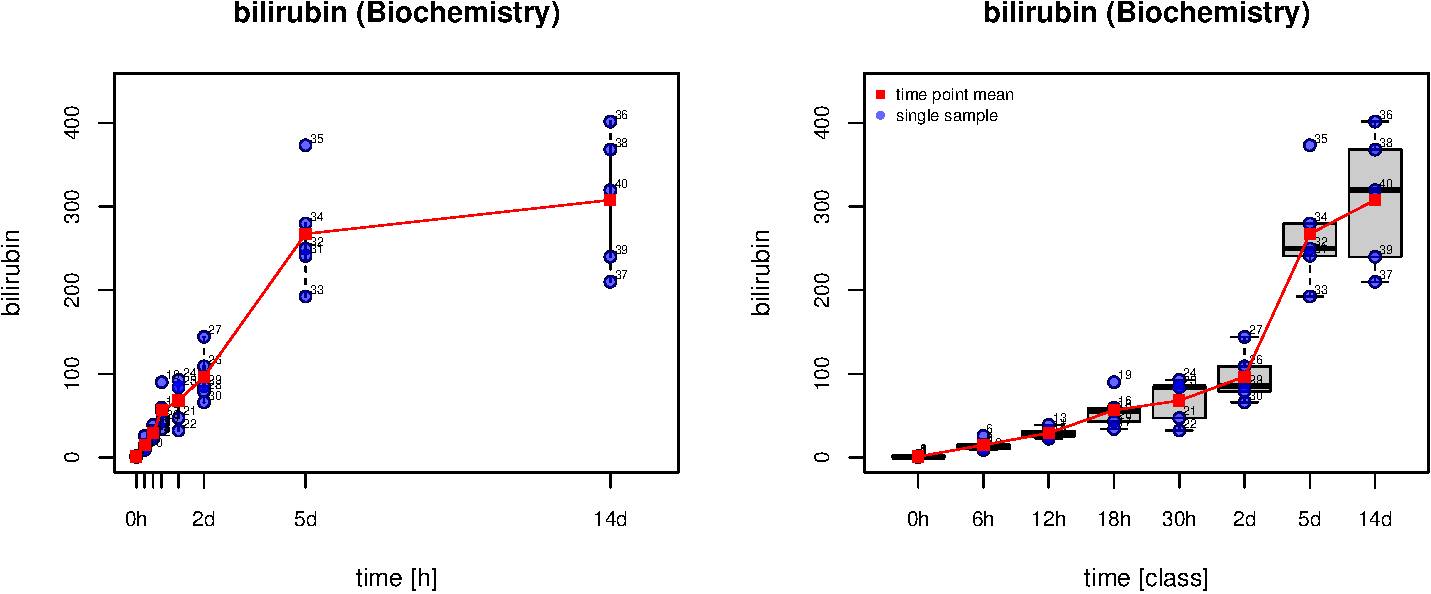
\includegraphics{Figs/bilirubin_plot-1.pdf}

Figure: Bilrubin timecourse. Plot of the raw time course data for
bilirubin. On the left the data is plotted against the time {[}h{]}, on
the right against the different time classes. Individual data points are
depecticed in blue with the respective sample number shown next to the
data points. The mean averaged of the repeats per time point are
depicted in red.

\subsubsection{Time course of all
factors}\label{time-course-of-all-factors}

Next the heatmap overview of the complete data set is generated,
i.e.~the data of all factors for of all time points and repeats. This
provides a first overview over the complete data set.

\begin{Shaded}
\begin{Highlighting}[]
\KeywordTok{suppressPackageStartupMessages}\NormalTok{(}\KeywordTok{library}\NormalTok{(gplots))}
\KeywordTok{suppressPackageStartupMessages}\NormalTok{(}\KeywordTok{library}\NormalTok{(RColorBrewer))}

\CommentTok{# define horizontal and vertical helper lines}
\NormalTok{v_lines <-}\StringTok{ }\NormalTok{((}\DecValTok{1}\NormalTok{:Nt)*Nr}\FloatTok{+0.5}\NormalTok{)}
\NormalTok{factor_types <-}\StringTok{ }\KeywordTok{c}\NormalTok{(}\StringTok{"Histochemistry"}\NormalTok{, }\StringTok{"Biochemistry"}\NormalTok{, }
                  \StringTok{"GE_Fibrosis"}\NormalTok{, }\StringTok{"GE_Cytokines"}\NormalTok{, }\StringTok{"GE_ADME"}\NormalTok{)}
\NormalTok{factor_table <-}\StringTok{ }\KeywordTok{table}\NormalTok{(BDLfactors$ftype)}
\NormalTok{h_lines <-}\StringTok{ }\FloatTok{0.5} \NormalTok{+}\StringTok{ }\KeywordTok{cumsum}\NormalTok{(factor_table[factor_types])}

\NormalTok{timecourse_heatmap <-}\StringTok{ }\NormalTok{function()\{}
  \CommentTok{# create better row names}
  \NormalTok{dtmp <-}\StringTok{ }\NormalTok{BDLdata}
  \KeywordTok{rownames}\NormalTok{(dtmp) <-}\StringTok{ }\KeywordTok{paste}\NormalTok{(}\KeywordTok{rownames}\NormalTok{(BDLsamples), BDLsamples$time_fac, }\DataTypeTok{sep=}\StringTok{" "}\NormalTok{)}
  \CommentTok{# heatmap colors }
  \NormalTok{hmap_colors <-}\StringTok{ }\KeywordTok{HeatmapColors}\NormalTok{()}
  \CommentTok{# colors for factor groups}
  \NormalTok{colorset <-}\StringTok{ }\KeywordTok{brewer.pal}\NormalTok{(}\KeywordTok{length}\NormalTok{(factor_types), }\StringTok{"Set2"}\NormalTok{)}
  \NormalTok{color.map <-}\StringTok{ }\NormalTok{function(factor_id) \{}
    \KeywordTok{return}\NormalTok{(}
      \NormalTok{colorset[}\KeywordTok{which}\NormalTok{(factor_types==BDLfactors$ftype[}\KeywordTok{which}\NormalTok{(BDLfactors$id==factor_id)])]}
    \NormalTok{)}
  \NormalTok{\}}
  \NormalTok{factorColors <-}\StringTok{ }\KeywordTok{unlist}\NormalTok{(}\KeywordTok{lapply}\NormalTok{(BDLfactors$id, color.map))}
  \CommentTok{# heatmap}
  \KeywordTok{heatmap.2}\NormalTok{(}\KeywordTok{t}\NormalTok{(}\KeywordTok{as.matrix}\NormalTok{(dtmp)), }\DataTypeTok{col=}\KeywordTok{hmap_colors}\NormalTok{(}\DecValTok{100}\NormalTok{), }\DataTypeTok{scale=}\StringTok{"row"}\NormalTok{, }
            \DataTypeTok{dendrogram=}\StringTok{"none"}\NormalTok{, }\DataTypeTok{Rowv=}\OtherTok{NULL}\NormalTok{, }\DataTypeTok{Colv=}\OtherTok{NULL}\NormalTok{,}
            \DataTypeTok{key=}\OtherTok{TRUE}\NormalTok{, }\DataTypeTok{trace=}\StringTok{"none"}\NormalTok{, }\DataTypeTok{cexRow=}\FloatTok{0.5}\NormalTok{, }\DataTypeTok{keysize=}\FloatTok{0.8}\NormalTok{, }\DataTypeTok{density.info=}\StringTok{"none"}\NormalTok{,}
            \DataTypeTok{RowSideColors=}\NormalTok{factorColors,}
            \DataTypeTok{add.expr=}\KeywordTok{abline}\NormalTok{(}\DataTypeTok{v=}\NormalTok{v_lines, }\DataTypeTok{h=}\NormalTok{h_lines, }\DataTypeTok{col=}\StringTok{"black"}\NormalTok{, }\DataTypeTok{lwd=}\FloatTok{0.5}\NormalTok{),}
            \DataTypeTok{main=}\StringTok{"Heatmap of BDL time course data"}\NormalTok{)}
            \CommentTok{# xlab="sample", ylab="factor")}
  \CommentTok{# legend}
  \KeywordTok{legend}\NormalTok{(}\StringTok{"left"}\NormalTok{,}
      \DataTypeTok{inset=}\KeywordTok{c}\NormalTok{(-}\FloatTok{0.03}\NormalTok{,}\DecValTok{0}\NormalTok{),}
      \DataTypeTok{legend =} \KeywordTok{rev}\NormalTok{(factor_types), }\CommentTok{# category labels}
      \DataTypeTok{col =} \KeywordTok{rev}\NormalTok{(colorset),  }\CommentTok{# color key}
      \DataTypeTok{lty=} \DecValTok{1}\NormalTok{, }\DataTypeTok{lwd =} \DecValTok{10}\NormalTok{, }\DataTypeTok{cex =} \FloatTok{0.7}\NormalTok{, }\DataTypeTok{bty=}\StringTok{"n"}
  \NormalTok{)}
\NormalTok{\}}
\CommentTok{# plot to file}
\KeywordTok{pdf}\NormalTok{(}\KeywordTok{file.path}\NormalTok{(resultsPath, }\StringTok{"control"}\NormalTok{, }\StringTok{"timecourse_heatmap.pdf"}\NormalTok{), }
    \DataTypeTok{width=}\DecValTok{10}\NormalTok{, }\DataTypeTok{height=}\DecValTok{10}\NormalTok{, }\DataTypeTok{pointsize=}\DecValTok{12}\NormalTok{) }
\KeywordTok{timecourse_heatmap}\NormalTok{()}
\KeywordTok{invisible}\NormalTok{(}\KeywordTok{dev.off}\NormalTok{())}
\end{Highlighting}
\end{Shaded}

\begin{Shaded}
\begin{Highlighting}[]
\KeywordTok{timecourse_heatmap}\NormalTok{()}
\end{Highlighting}
\end{Shaded}

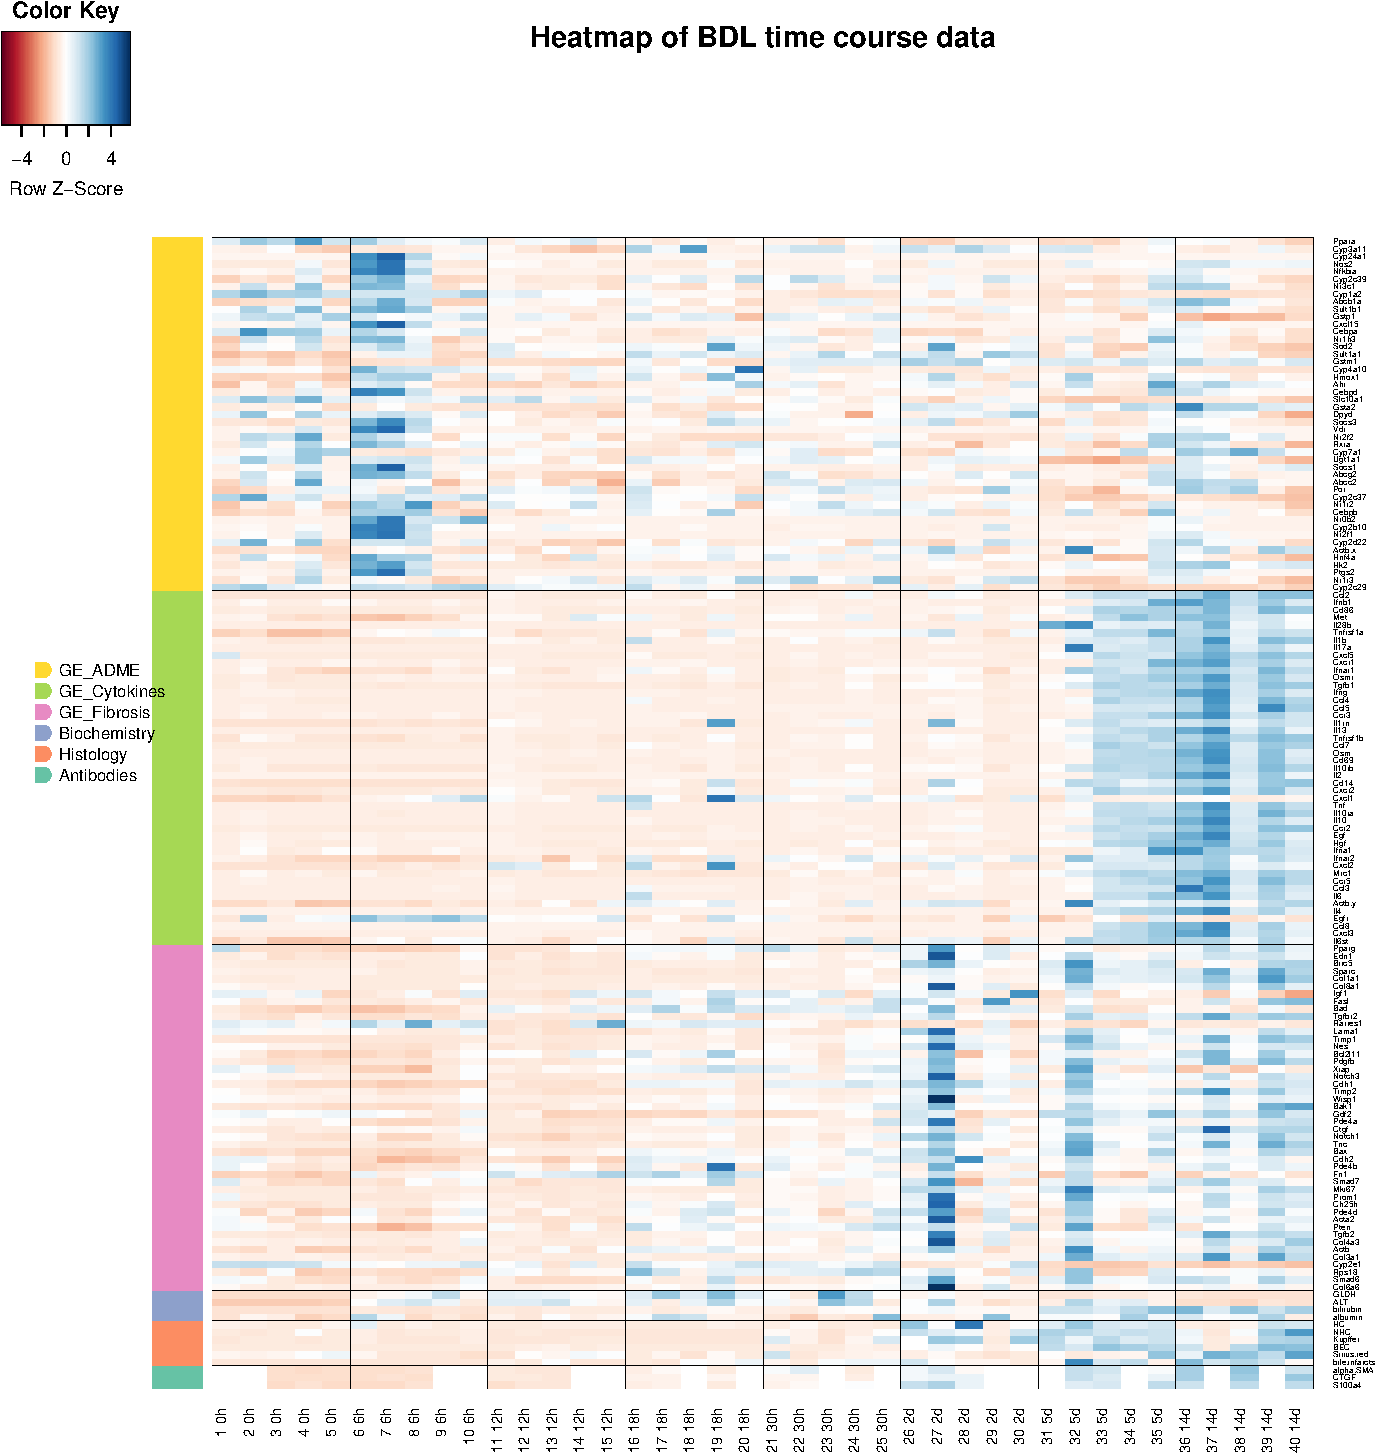
\includegraphics{Figs/timecourse_heatmap_report-1.pdf}

Figure: Timecourse heatmap of all factors. Rows correspond to individual
factors, with factor order corresponding to the original data set:
\texttt{GE\_ADME}, \texttt{GE\_Cytokines}, \texttt{GE\_Fibrosis},
\texttt{Biochemistry}, \texttt{Histochemistry}. Columns correspond to
the 40 samples with 5 subsequent samples belonging to one of the 8 time
points. The data is row scaled, i.e.~every individual factor is scaled
to have mean zero and standard deviation one.

\textbf{Results}: Various patterns are visible in the plotted raw data
set:

\begin{itemize}
\itemsep1pt\parskip0pt\parsep0pt
\item
  \textbf{Two main classes of time course response are observed}. One
  class with an increase in the early phase up to 6h after BDL (many of
  the ADME genes fall in this class) and a second class increasing in
  the later stage after 2-5 days after BDL. Many of the genes on the
  Cytokines and Fibrosis chips as well as some of the biochemical and
  (immuno-)histochemical factors fall in this second class.
\item
  \textbf{The individual animals show heterogeneous responses to BDL}.
  Within one time point the 5 repeats can show very different patterns.
  For instance at time 6h after BDL 3/5 of the mice show a marked
  increase in the ADME genes, whereas 2/5 do not show such a marked
  increase. Another example is the mice sample 27 at time 2d, with a
  high increase in the genes on the Fibrosis chip, which is not observed
  in the other 4 samples at time 2d.
\end{itemize}

\subsection{Actb quality control}\label{actb-quality-control}

Actb (Actin, cytoplasmic 1) probes were included on all Fluidigm chips
(\texttt{GE\_ADME}, \texttt{GE\_Cytokines}, \texttt{GE\_Fibrosis}) and
not used in the normalization of the transcription data. Hence, ActB can
serve as quality control for the technical reproducibility of the
Fluidigm chips. If the data is reproducible between chips the pairwise
correlation between all individual Actb measurements should have high
correlation coefficients close to 1. Plotting the data of the Actb
measurements of two chips against each other should lie on a straight
line.

\begin{Shaded}
\begin{Highlighting}[]
\CommentTok{# Actb control figure}
\NormalTok{plot_actb_control <-}\StringTok{ }\NormalTok{function()\{}
  \KeywordTok{par}\NormalTok{(}\DataTypeTok{mfrow=}\KeywordTok{c}\NormalTok{(}\DecValTok{2}\NormalTok{,}\DecValTok{3}\NormalTok{))}
  \KeywordTok{plot_single}\NormalTok{(}\StringTok{"Actb"}\NormalTok{)}
  \KeywordTok{plot_single}\NormalTok{(}\StringTok{"Actb.x"}\NormalTok{)}
  \KeywordTok{plot_single}\NormalTok{(}\StringTok{"Actb.y"}\NormalTok{)}
  \KeywordTok{plot_cor_pair}\NormalTok{(}\StringTok{"Actb"}\NormalTok{, }\StringTok{"Actb.x"}\NormalTok{, }\DataTypeTok{single_plots=}\OtherTok{FALSE}\NormalTok{)}
  \KeywordTok{plot_cor_pair}\NormalTok{(}\StringTok{"Actb"}\NormalTok{, }\StringTok{"Actb.y"}\NormalTok{, }\DataTypeTok{single_plots=}\OtherTok{FALSE}\NormalTok{)}
  \KeywordTok{plot_cor_pair}\NormalTok{(}\StringTok{"Actb.x"}\NormalTok{, }\StringTok{"Actb.y"}\NormalTok{, }\DataTypeTok{single_plots=}\OtherTok{FALSE}\NormalTok{)}
  \KeywordTok{par}\NormalTok{(}\DataTypeTok{mfrow=}\KeywordTok{c}\NormalTok{(}\DecValTok{1}\NormalTok{,}\DecValTok{1}\NormalTok{))}
\NormalTok{\}}

\CommentTok{# plot to file}
\KeywordTok{pdf}\NormalTok{(}\KeywordTok{file.path}\NormalTok{(resultsPath, }\StringTok{"control"}\NormalTok{, }\StringTok{"Actb_control.pdf"}\NormalTok{), }
    \DataTypeTok{width=}\DecValTok{10}\NormalTok{, }\DataTypeTok{height=}\DecValTok{6}\NormalTok{, }\DataTypeTok{pointsize=}\DecValTok{12}\NormalTok{)  }
\KeywordTok{plot_actb_control}\NormalTok{()}
\KeywordTok{invisible}\NormalTok{(}\KeywordTok{dev.off}\NormalTok{())}

\CommentTok{# calculate Spearman and Pearson correlation coefficients on N=8*5=40 data points }
\NormalTok{actb.spearman <-}\StringTok{ }\KeywordTok{cor}\NormalTok{(}\KeywordTok{data.frame}\NormalTok{(}\DataTypeTok{Actb=}\NormalTok{BDLdata$Actb, }
                                \DataTypeTok{Actb.x=}\NormalTok{BDLdata$Actb.x, }
                                \DataTypeTok{Actb.y=}\NormalTok{BDLdata$Actb.y), }\DataTypeTok{method=}\StringTok{"spearman"}\NormalTok{)}
\NormalTok{actb.pearson <-}\StringTok{ }\KeywordTok{cor}\NormalTok{(}\KeywordTok{data.frame}\NormalTok{(}\DataTypeTok{Actb=}\NormalTok{BDLdata$Actb, }
                               \DataTypeTok{Actb.x=}\NormalTok{BDLdata$Actb.x, }
                               \DataTypeTok{Actb.y=}\NormalTok{BDLdata$Actb.y), }\DataTypeTok{method=}\StringTok{"pearson"}\NormalTok{)}

\CommentTok{# table of correlation coefficients}
\KeywordTok{set.caption}\NormalTok{(}\KeywordTok{sub}\NormalTok{(}\StringTok{"."}\NormalTok{, }\StringTok{" "}\NormalTok{, }\StringTok{"Spearman correlation of Actb controls"}\NormalTok{, }\DataTypeTok{fixed =} \OtherTok{TRUE}\NormalTok{))}
\KeywordTok{pander}\NormalTok{(}\KeywordTok{round}\NormalTok{(actb.spearman, }\DataTypeTok{digits=}\DecValTok{3}\NormalTok{))}
\end{Highlighting}
\end{Shaded}

\begin{longtable}[c]{@{}cccc@{}}
\caption{Spearman correlation of Actb controls}\tabularnewline
\toprule
\begin{minipage}[b]{0.16\columnwidth}\centering\strut
~
\strut\end{minipage} &
\begin{minipage}[b]{0.09\columnwidth}\centering\strut
Actb
\strut\end{minipage} &
\begin{minipage}[b]{0.11\columnwidth}\centering\strut
Actb.x
\strut\end{minipage} &
\begin{minipage}[b]{0.11\columnwidth}\centering\strut
Actb.y
\strut\end{minipage}\tabularnewline
\midrule
\endfirsthead
\toprule
\begin{minipage}[b]{0.16\columnwidth}\centering\strut
~
\strut\end{minipage} &
\begin{minipage}[b]{0.09\columnwidth}\centering\strut
Actb
\strut\end{minipage} &
\begin{minipage}[b]{0.11\columnwidth}\centering\strut
Actb.x
\strut\end{minipage} &
\begin{minipage}[b]{0.11\columnwidth}\centering\strut
Actb.y
\strut\end{minipage}\tabularnewline
\midrule
\endhead
\begin{minipage}[t]{0.16\columnwidth}\centering\strut
\textbf{Actb}
\strut\end{minipage} &
\begin{minipage}[t]{0.09\columnwidth}\centering\strut
1
\strut\end{minipage} &
\begin{minipage}[t]{0.11\columnwidth}\centering\strut
0.908
\strut\end{minipage} &
\begin{minipage}[t]{0.11\columnwidth}\centering\strut
0.944
\strut\end{minipage}\tabularnewline
\begin{minipage}[t]{0.16\columnwidth}\centering\strut
\textbf{Actb.x}
\strut\end{minipage} &
\begin{minipage}[t]{0.09\columnwidth}\centering\strut
0.908
\strut\end{minipage} &
\begin{minipage}[t]{0.11\columnwidth}\centering\strut
1
\strut\end{minipage} &
\begin{minipage}[t]{0.11\columnwidth}\centering\strut
0.917
\strut\end{minipage}\tabularnewline
\begin{minipage}[t]{0.16\columnwidth}\centering\strut
\textbf{Actb.y}
\strut\end{minipage} &
\begin{minipage}[t]{0.09\columnwidth}\centering\strut
0.944
\strut\end{minipage} &
\begin{minipage}[t]{0.11\columnwidth}\centering\strut
0.917
\strut\end{minipage} &
\begin{minipage}[t]{0.11\columnwidth}\centering\strut
1
\strut\end{minipage}\tabularnewline
\bottomrule
\end{longtable}

\begin{Shaded}
\begin{Highlighting}[]
\KeywordTok{set.caption}\NormalTok{(}\KeywordTok{sub}\NormalTok{(}\StringTok{"."}\NormalTok{, }\StringTok{" "}\NormalTok{, }\StringTok{"Pearson correlation of Actb controls"}\NormalTok{, }\DataTypeTok{fixed =} \OtherTok{TRUE}\NormalTok{))}
\KeywordTok{pander}\NormalTok{(}\KeywordTok{round}\NormalTok{(actb.pearson, }\DataTypeTok{digits=}\DecValTok{3}\NormalTok{))}
\end{Highlighting}
\end{Shaded}

\begin{longtable}[c]{@{}cccc@{}}
\caption{Pearson correlation of Actb controls}\tabularnewline
\toprule
\begin{minipage}[b]{0.16\columnwidth}\centering\strut
~
\strut\end{minipage} &
\begin{minipage}[b]{0.09\columnwidth}\centering\strut
Actb
\strut\end{minipage} &
\begin{minipage}[b]{0.11\columnwidth}\centering\strut
Actb.x
\strut\end{minipage} &
\begin{minipage}[b]{0.11\columnwidth}\centering\strut
Actb.y
\strut\end{minipage}\tabularnewline
\midrule
\endfirsthead
\toprule
\begin{minipage}[b]{0.16\columnwidth}\centering\strut
~
\strut\end{minipage} &
\begin{minipage}[b]{0.09\columnwidth}\centering\strut
Actb
\strut\end{minipage} &
\begin{minipage}[b]{0.11\columnwidth}\centering\strut
Actb.x
\strut\end{minipage} &
\begin{minipage}[b]{0.11\columnwidth}\centering\strut
Actb.y
\strut\end{minipage}\tabularnewline
\midrule
\endhead
\begin{minipage}[t]{0.16\columnwidth}\centering\strut
\textbf{Actb}
\strut\end{minipage} &
\begin{minipage}[t]{0.09\columnwidth}\centering\strut
1
\strut\end{minipage} &
\begin{minipage}[t]{0.11\columnwidth}\centering\strut
0.945
\strut\end{minipage} &
\begin{minipage}[t]{0.11\columnwidth}\centering\strut
0.938
\strut\end{minipage}\tabularnewline
\begin{minipage}[t]{0.16\columnwidth}\centering\strut
\textbf{Actb.x}
\strut\end{minipage} &
\begin{minipage}[t]{0.09\columnwidth}\centering\strut
0.945
\strut\end{minipage} &
\begin{minipage}[t]{0.11\columnwidth}\centering\strut
1
\strut\end{minipage} &
\begin{minipage}[t]{0.11\columnwidth}\centering\strut
0.935
\strut\end{minipage}\tabularnewline
\begin{minipage}[t]{0.16\columnwidth}\centering\strut
\textbf{Actb.y}
\strut\end{minipage} &
\begin{minipage}[t]{0.09\columnwidth}\centering\strut
0.938
\strut\end{minipage} &
\begin{minipage}[t]{0.11\columnwidth}\centering\strut
0.935
\strut\end{minipage} &
\begin{minipage}[t]{0.11\columnwidth}\centering\strut
1
\strut\end{minipage}\tabularnewline
\bottomrule
\end{longtable}

\begin{Shaded}
\begin{Highlighting}[]
\KeywordTok{plot_actb_control}\NormalTok{()}
\end{Highlighting}
\end{Shaded}

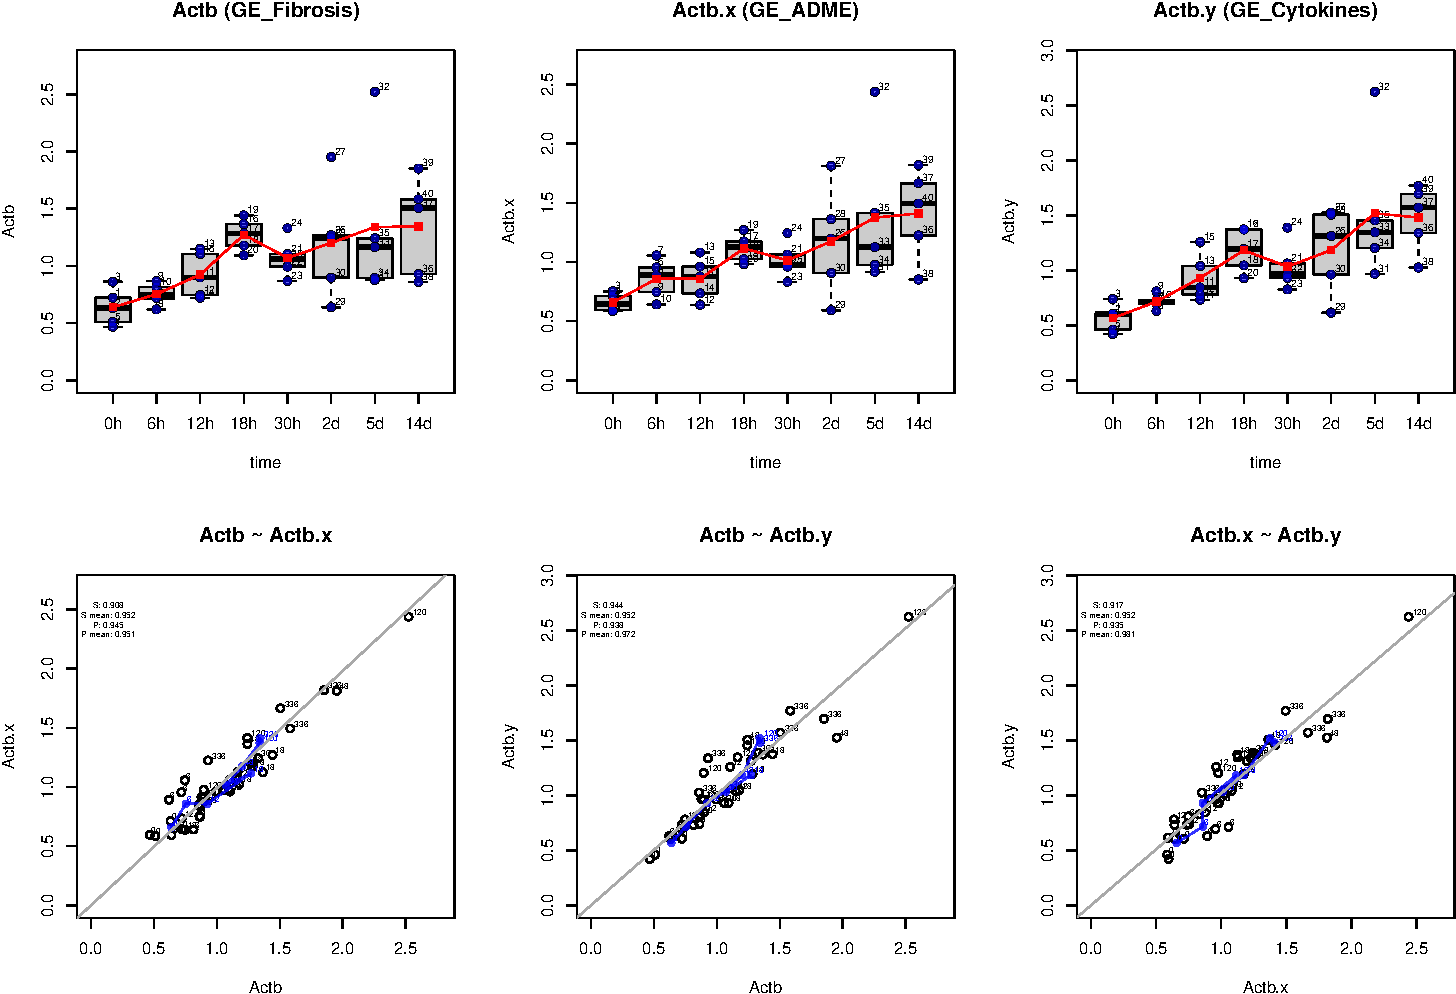
\includegraphics{Figs/actb_control_plot-1.pdf}

Figure: Actb control. Correlation plot of the Actb probes from the 3
Fluidigm chips: Actb (fibrosis), Actb.x (ADME), Actb.y (Cytokines). The
top row shows the individual time courses, the bottom row the pair wise
plot of individual data points.

\textbf{Results}: The Actb Fluidigm gene expression measurements are
highly reproducible for the measured chips, with Spearman as well as
Pearson correlation coefficients all \textgreater{} 0.9 for pairwise
Actb comparison.

\section{Dimension reduction}\label{dimension-reduction}

A one-way analysis of variance (ANOVA) was applied to reduce the factors
to the subset showing significant (\(p_{adj}< 0.05\)) changes during the
time course. In its simplest form, ANOVA provides a statistical test of
whether or not the means of several groups are equal, and therefore
generalizes the t-test to more than two groups, with the groups being
the sampled time points. The Holm's procedure was used to correct the
p-values for any artificial p-value inflation due to multiple testing.

In a first step, an ANOVA was calculated with the groups corresponding
to the different time points for every factor in the BDL data set.
Dimension reduction was than performed by filtering out those factors
which did not significantly change over time.

The \texttt{BDLdata} data set is reshaped into matrix format for the
ANOVA calculation, with time points in rows and repeats as columns for
every factor.

\begin{Shaded}
\begin{Highlighting}[]
\NormalTok{BDLmatrices <-}\StringTok{ }\KeywordTok{bdl_matrix_data}\NormalTok{(BDLdata, BDLsamples)}
\end{Highlighting}
\end{Shaded}

\subsection{ANOVA for single factor}\label{anova-for-single-factor}

The following shows the ANOVA calculation for a single factor. We use
again the example \texttt{bilirubin} to demonstrate the method.

\begin{Shaded}
\begin{Highlighting}[]
  \CommentTok{# example ANOVA for one factor}
  \NormalTok{mat.anova <-}\StringTok{ }\KeywordTok{t}\NormalTok{(BDLmatrices[[}\StringTok{'bilirubin'}\NormalTok{]])}
  \KeywordTok{colnames}\NormalTok{(mat.anova) <-}\StringTok{ }\KeywordTok{levels}\NormalTok{(BDLsamples$time_fac)}
  \KeywordTok{print}\NormalTok{(mat.anova)}
\end{Highlighting}
\end{Shaded}

\begin{verbatim}
     0h    6h   12h   18h   30h     2d    5d   14d
R1 1.49 25.80 31.51 59.40 47.11 108.95 241.0 401.5
R2 0.93 13.87 22.51 33.95 32.26 144.20 249.8 210.0
R3 1.65 10.70 38.99 55.80 83.98  79.10 192.5 368.0
R4 0.85 15.08 25.81 90.05 92.72  85.10 279.7 239.9
R5 0.53  8.96 27.21 43.30 84.02  65.95 373.2 319.5
\end{verbatim}

\begin{Shaded}
\begin{Highlighting}[]
  \CommentTok{# concatenate the data rows of df1 into a single vector r .}
  \NormalTok{r =}\StringTok{ }\KeywordTok{c}\NormalTok{(}\KeywordTok{t}\NormalTok{(}\KeywordTok{as.matrix}\NormalTok{(mat.anova)))  }\CommentTok{# response data }
  
  \CommentTok{# assign new variables for the treatment levels and number of observations.}
  \NormalTok{f =}\StringTok{ }\KeywordTok{levels}\NormalTok{(BDLsamples$time_fac)   }\CommentTok{# treatment levels }
  \NormalTok{k =}\StringTok{ }\NormalTok{Nt                             }\CommentTok{# number of treatment levels (time points Nt=8) }
  \NormalTok{n =}\StringTok{ }\NormalTok{Nr                             }\CommentTok{# observations per treatment (repeats Nr=5)}
  
  \CommentTok{# vector of treatment factors that corresponds to each element of r }
  \CommentTok{# in step 3 with the gl function.}
  \NormalTok{tm <-}\StringTok{ }\KeywordTok{gl}\NormalTok{(k, }\DecValTok{1}\NormalTok{, n*k, }\KeywordTok{factor}\NormalTok{(f))   }\CommentTok{# matching treatments }
  
  \CommentTok{# apply the function aov to a formula that describes the response r }
  \CommentTok{# by the treatment factor tm (fit ANOVA model)}
  \NormalTok{av <-}\StringTok{ }\KeywordTok{aov}\NormalTok{(r ~}\StringTok{ }\NormalTok{tm) }
  
  \CommentTok{# print ANOVA summary}
  \KeywordTok{summary}\NormalTok{(av)}
\end{Highlighting}
\end{Shaded}

\begin{verbatim}
            Df Sum Sq Mean Sq F value   Pr(>F)    
tm           7 479470   68496      41 3.27e-14 ***
Residuals   32  53463    1671                     
---
Signif. codes:  0 '***' 0.001 '**' 0.01 '*' 0.05 '.' 0.1 ' ' 1
\end{verbatim}

\begin{Shaded}
\begin{Highlighting}[]
  \CommentTok{# print p-value}
  \NormalTok{p.value <-}\StringTok{ }\KeywordTok{summary}\NormalTok{(av)[[}\DecValTok{1}\NormalTok{]][[}\StringTok{"Pr(>F)"}\NormalTok{]][[}\DecValTok{1}\NormalTok{]]}
\end{Highlighting}
\end{Shaded}

\textbf{Results:} The time course fo bilirubin is highly altered after
BDL, resulting in a high significance of the ANOVA. This confirms what
we saw in the initial visual inspection of bilirubin (see Figure above).

\subsection{ANOVA for all factors}\label{anova-for-all-factors}

The ANOVA calculation for all individual factors is performed analog to
the calculate for bilirubin. As a consequence of the large number of
factors, a multitude of tests are performed, namely an ANOVA for every
single factor. Consequently, the reported p-values of the ANOVA have to
be adjusted for multiple testing. This is done using the
\texttt{p.adjust} function which given a set of p-values, returns
p-values adjusted using one of several methods. We selected the Holm's
method designed to give strong control of the family-wise error rate
(\emph{Holm, S. (1979). A simple sequentially rejective multiple test
procedure. Scandinavian Journal of Statistics 6, 65-70.}).

\begin{Shaded}
\begin{Highlighting}[]
\CommentTok{# Calculation of ANOVA for all factors}
\NormalTok{df.anova <-}\StringTok{ }\KeywordTok{all_factor_anova}\NormalTok{()}
\NormalTok{df.anova$sig <-}\StringTok{ }\KeywordTok{sapply}\NormalTok{(df.anova$p.value, significant_code)  }\CommentTok{# add significant codes}

\NormalTok{df.anova$p.holm <-}\StringTok{ }\KeywordTok{p.adjust}\NormalTok{(df.anova$p.value, }\DataTypeTok{method =}\StringTok{"holm"}\NormalTok{, }
                            \DataTypeTok{n =} \KeywordTok{length}\NormalTok{(df.anova$p.value))}
\NormalTok{df.anova$sig.holm <-}\StringTok{ }\KeywordTok{sapply}\NormalTok{(df.anova$p.holm, significant_code) }
\NormalTok{df.anova$ftype <-}\StringTok{ }\NormalTok{BDLfactors$ftype}
\NormalTok{df.anova$fshort <-}\StringTok{ }\NormalTok{BDLfactors$ftype.short}

\CommentTok{# order factors by adjusted p-values, and cleanup for printing}
\NormalTok{df.anova.ordered <-}\StringTok{ }\NormalTok{df.anova[}\KeywordTok{with}\NormalTok{(df.anova, }\KeywordTok{order}\NormalTok{(p.holm)), ]}
\KeywordTok{rownames}\NormalTok{(df.anova.ordered) <-}\StringTok{ }\NormalTok{df.anova.ordered$factors}
\NormalTok{df.anova.ordered <-}\StringTok{ }\NormalTok{df.anova.ordered[}\KeywordTok{c}\NormalTok{(}\StringTok{"p.holm"}\NormalTok{, }\StringTok{"sig.holm"}\NormalTok{, }\StringTok{"ftype"}\NormalTok{, }\StringTok{"fshort"}\NormalTok{)]}
\NormalTok{df.anova.ordered$p.holm <-}\StringTok{ }\KeywordTok{as.numeric}\NormalTok{(}\KeywordTok{sprintf}\NormalTok{(}\StringTok{"%1.2E"}\NormalTok{, df.anova.ordered$p.holm))}

\CommentTok{# save results}
\KeywordTok{write.table}\NormalTok{(df.anova.ordered, }\DataTypeTok{file=}\KeywordTok{file.path}\NormalTok{(resultsPath, }\StringTok{"data"}\NormalTok{, }\StringTok{'BDLanova.csv'}\NormalTok{), }
            \DataTypeTok{sep=}\StringTok{"}\CharTok{\textbackslash{}t}\StringTok{"}\NormalTok{, }\DataTypeTok{quote=}\OtherTok{FALSE}\NormalTok{)}
\KeywordTok{save}\NormalTok{(df.anova, }\DataTypeTok{file=}\KeywordTok{file.path}\NormalTok{(resultsPath, }\StringTok{"data"}\NormalTok{, }\StringTok{"BDLanova.Rdata"}\NormalTok{))}
\end{Highlighting}
\end{Shaded}

\small

\begin{Shaded}
\begin{Highlighting}[]
\KeywordTok{print}\NormalTok{(df.anova.ordered)}
\end{Highlighting}
\end{Shaded}

\begin{verbatim}
                p.holm sig.holm          ftype fshort
Cyp1a2        2.93e-14      ***        GE_ADME       
bilirubin     4.98e-12      ***   Biochemistry      B
Il10rb        1.15e-11      ***   GE_Cytokines       
Tgfb1         3.30e-11      ***   GE_Cytokines       
Ccl2          3.46e-11      ***   GE_Cytokines       
Cd86          6.56e-11      ***   GE_Cytokines       
Ccr2          6.94e-11      ***   GE_Cytokines       
Mrc1          6.95e-11      ***   GE_Cytokines       
Tnfrsf1b      7.89e-11      ***   GE_Cytokines       
Cxcl5         6.26e-10      ***   GE_Cytokines       
CTGF          7.82e-10      *** Histochemistry      H
Il10ra        1.64e-09      ***   GE_Cytokines       
Gstm1         9.18e-09      ***        GE_ADME       
Ccl7          3.40e-08      ***   GE_Cytokines       
Ccr5          4.36e-08      ***   GE_Cytokines       
Hgf           5.80e-08      ***   GE_Cytokines       
Osmr          1.01e-07      ***   GE_Cytokines       
Ccl4          1.04e-07      ***   GE_Cytokines       
Nr0b2         1.30e-07      ***        GE_ADME       
Tgfbr2        1.71e-07      ***    GE_Fibrosis       
BEC           2.09e-07      *** Histochemistry      H
Ccl5          2.78e-07      ***   GE_Cytokines       
Col1a1        4.40e-07      ***    GE_Fibrosis       
Ifnar1        7.71e-07      ***   GE_Cytokines       
S100a4        9.19e-07      *** Histochemistry      H
Sparc         1.07e-06      ***    GE_Fibrosis       
Cyp2e1        1.50e-06      ***    GE_Fibrosis       
Cxcr2         1.75e-06      ***   GE_Cytokines       
Ccr3          1.91e-06      ***   GE_Cytokines       
Cd69          2.73e-06      ***   GE_Cytokines       
Cyp2c29       2.93e-06      ***        GE_ADME       
Gsta2         3.88e-06      ***        GE_ADME       
Tnf           4.36e-06      ***   GE_Cytokines       
Gdf2          5.95e-06      ***    GE_Fibrosis       
Il1b          7.29e-06      ***   GE_Cytokines       
Ifng          7.51e-06      ***   GE_Cytokines       
Osm           7.51e-06      ***   GE_Cytokines       
Ccl3          8.53e-06      ***   GE_Cytokines       
Il13          9.29e-06      ***   GE_Cytokines       
Cxcr1         1.07e-05      ***   GE_Cytokines       
Cyp2c37       1.09e-05      ***        GE_ADME       
Cd14          1.15e-05      ***   GE_Cytokines       
Col3a1        2.02e-05      ***    GE_Fibrosis       
Tnfrsf1a      3.33e-05      ***   GE_Cytokines       
Il2           4.84e-05      ***   GE_Cytokines       
Ifnb1         4.86e-05      ***   GE_Cytokines       
Egf           4.88e-05      ***   GE_Cytokines       
Il28b         4.88e-05      ***   GE_Cytokines       
Il10          4.88e-05      ***   GE_Cytokines       
Il4           4.88e-05      ***   GE_Cytokines       
Slc10a1       5.26e-05      ***        GE_ADME       
Timp2         6.24e-05      ***    GE_Fibrosis       
Cxcl3         6.82e-05      ***   GE_Cytokines       
Ccl8          1.23e-04      ***   GE_Cytokines       
Ctgf          1.32e-04      ***    GE_Fibrosis       
Gstp1         1.38e-04      ***        GE_ADME       
Ppara         1.63e-04      ***        GE_ADME       
Ifnar2        1.82e-04      ***   GE_Cytokines       
Il6           2.23e-04      ***   GE_Cytokines       
Il17a         2.43e-04      ***   GE_Cytokines       
Bad           3.84e-04      ***    GE_Fibrosis       
Timp1         4.30e-04      ***    GE_Fibrosis       
Cdh1          4.48e-04      ***    GE_Fibrosis       
Cebpa         4.93e-04      ***        GE_ADME       
alpha.SMA     5.02e-04      *** Histochemistry      H
NPC           5.28e-04      *** Histochemistry      H
Cdh2          5.38e-04      ***    GE_Fibrosis       
Sirius.red    7.59e-04      *** Histochemistry      H
Pdgfb         7.68e-04      ***    GE_Fibrosis       
Il6st         8.71e-04      ***   GE_Cytokines       
Fn1           1.21e-03       **    GE_Fibrosis       
Mki67         1.46e-03       **    GE_Fibrosis       
Ifna1         1.46e-03       **   GE_Cytokines       
Egfr          1.59e-03       **   GE_Cytokines       
Kupffer       1.95e-03       ** Histochemistry      H
Tnc           2.04e-03       **    GE_Fibrosis       
Ugt1a1        2.75e-03       **        GE_ADME       
Sult1a1       2.98e-03       **        GE_ADME       
GLDH          4.28e-03       **   Biochemistry      B
Notch1        4.45e-03       **    GE_Fibrosis       
Met           4.97e-03       **   GE_Cytokines       
Cyp7a1        9.83e-03       **        GE_ADME       
Cyp24a1       9.88e-03       **        GE_ADME       
Tgfb2         1.08e-02        *    GE_Fibrosis       
Birc5         1.69e-02        *    GE_Fibrosis       
Actb.y        1.91e-02        *   GE_Cytokines       
Bak1          2.73e-02        *    GE_Fibrosis       
Bax           2.89e-02        *    GE_Fibrosis       
Rarres1       3.57e-02        *    GE_Fibrosis       
bile.infarcts 3.78e-02        * Histochemistry      H
Cyp3a11       5.30e-02        .        GE_ADME       
Sult1b1       5.74e-02        .        GE_ADME       
Cyp4a10       6.79e-02        .        GE_ADME       
Pparg         6.79e-02        .    GE_Fibrosis       
Hk2           7.50e-02        .        GE_ADME       
ALT           8.79e-02        .   Biochemistry      B
Smad6         9.49e-02        .    GE_Fibrosis       
Cyp2b10       1.17e-01                 GE_ADME       
HC            1.27e-01          Histochemistry      H
Il1rn         1.35e-01            GE_Cytokines       
Nes           1.37e-01             GE_Fibrosis       
Nfkbia        1.57e-01                 GE_ADME       
Rps18         1.68e-01             GE_Fibrosis       
Cxcl15        2.18e-01                 GE_ADME       
Socs3         2.43e-01                 GE_ADME       
Vdr           2.43e-01                 GE_ADME       
Edn1          2.43e-01             GE_Fibrosis       
Nr2f1         2.63e-01                 GE_ADME       
Abcg2         2.82e-01                 GE_ADME       
Nr1i3         2.82e-01                 GE_ADME       
Hnf4a         2.88e-01                 GE_ADME       
Ptgs2         3.43e-01                 GE_ADME       
Bcl2l11       3.43e-01             GE_Fibrosis       
Socs1         3.46e-01                 GE_ADME       
Pten          3.66e-01             GE_Fibrosis       
Actb.x        3.90e-01                 GE_ADME       
Cxcl2         4.06e-01            GE_Cytokines       
Xiap          4.06e-01             GE_Fibrosis       
Pde4a         4.42e-01             GE_Fibrosis       
Dpyd          4.43e-01                 GE_ADME       
Cxcl1         4.43e-01            GE_Cytokines       
Lama1         4.57e-01             GE_Fibrosis       
Col8a1        5.07e-01             GE_Fibrosis       
Prom1         5.54e-01             GE_Fibrosis       
Actb          5.54e-01             GE_Fibrosis       
Ahr           5.57e-01                 GE_ADME       
Nr2f2         5.57e-01                 GE_ADME       
Nos2          5.82e-01                 GE_ADME       
Notch3        7.26e-01             GE_Fibrosis       
Cebpd         7.29e-01                 GE_ADME       
Hmox1         7.69e-01                 GE_ADME       
Cyp2d22       8.36e-01                 GE_ADME       
Igf1          9.78e-01             GE_Fibrosis       
Fasl          9.78e-01             GE_Fibrosis       
Cyp2c39       1.00e+00                 GE_ADME       
Nr3c1         1.00e+00                 GE_ADME       
Abcb1a        1.00e+00                 GE_ADME       
Nr1h3         1.00e+00                 GE_ADME       
Sod2          1.00e+00                 GE_ADME       
Rxra          1.00e+00                 GE_ADME       
Abcc2         1.00e+00                 GE_ADME       
Por           1.00e+00                 GE_ADME       
Nr1i2         1.00e+00                 GE_ADME       
Cebpb         1.00e+00                 GE_ADME       
Wisp1         1.00e+00             GE_Fibrosis       
Pde4b         1.00e+00             GE_Fibrosis       
Smad7         1.00e+00             GE_Fibrosis       
Ch25h         1.00e+00             GE_Fibrosis       
Pde4d         1.00e+00             GE_Fibrosis       
Acta2         1.00e+00             GE_Fibrosis       
Col4a3        1.00e+00             GE_Fibrosis       
Col6a6        1.00e+00             GE_Fibrosis       
albumin       1.00e+00            Biochemistry      B
\end{verbatim}

\normalsize

\subsection{Filter factors}\label{filter-factors}

The factors are now filtered based on the respective acceptance level of
the ANOVA, with the cutoff for the adjusted p-value, i.e.~all factors
with a ANOVA with \(p_{adj} \ge p_{accept}\) are filtered out. The
filtered raw data is available as \texttt{BDLdata.fil}, the filtered
mean data is stored as \texttt{BDLmean.fil}.

\begin{Shaded}
\begin{Highlighting}[]
\NormalTok{p.accept =}\StringTok{ }\FloatTok{0.05}  \CommentTok{# acceptance level}
\NormalTok{anova.accept =}\StringTok{ }\NormalTok{(df.anova$p.holm <}\StringTok{ }\NormalTok{p.accept)  }\CommentTok{# accepted subset}
\CommentTok{# subset of filtered data}
\NormalTok{BDLdata.fil <-}\StringTok{ }\NormalTok{BDLdata[, anova.accept]}
\NormalTok{BDLmean.fil <-}\StringTok{ }\NormalTok{BDLdata[, anova.accept]}

\CommentTok{# accepted}
\KeywordTok{table}\NormalTok{(anova.accept)  }\CommentTok{# 64 rejected / 90 accepted (adjusted)}
\end{Highlighting}
\end{Shaded}

\begin{verbatim}
anova.accept
FALSE  TRUE 
   63    90 
\end{verbatim}

\begin{Shaded}
\begin{Highlighting}[]
\CommentTok{# which factors are accepted in which category}
\NormalTok{fil_tab <-}\StringTok{ }\KeywordTok{data.frame}\NormalTok{(}
  \KeywordTok{table}\NormalTok{(BDLfactors$ftype[anova.accept]),}
  \KeywordTok{table}\NormalTok{(BDLfactors$ftype),}
  \KeywordTok{round}\NormalTok{(}\KeywordTok{table}\NormalTok{(BDLfactors$ftype[anova.accept])/}\KeywordTok{table}\NormalTok{(BDLfactors$ftype), }\DecValTok{2}\NormalTok{)}
\NormalTok{)}
\NormalTok{fil_tab <-}\StringTok{ }\NormalTok{fil_tab[, }\KeywordTok{c}\NormalTok{(}\StringTok{'Var1'}\NormalTok{, }\StringTok{'Freq'}\NormalTok{, }\StringTok{'Freq.1'}\NormalTok{, }\StringTok{'Freq.2'}\NormalTok{)]}
\KeywordTok{names}\NormalTok{(fil_tab) <-}\StringTok{ }\KeywordTok{c}\NormalTok{(}\StringTok{'Category'}\NormalTok{, }\StringTok{'Accepted'}\NormalTok{, }\StringTok{'All'}\NormalTok{, }\StringTok{'Percent'}\NormalTok{)}
\CommentTok{# overview of filtered factors}
\KeywordTok{print}\NormalTok{(fil_tab)}
\end{Highlighting}
\end{Shaded}

\begin{verbatim}
        Category Accepted All Percent
1   Biochemistry        2   4    0.50
2        GE_ADME       14  47    0.30
3   GE_Cytokines       44  47    0.94
4    GE_Fibrosis       22  46    0.48
5 Histochemistry        8   9    0.89
\end{verbatim}

\begin{Shaded}
\begin{Highlighting}[]
\KeywordTok{rm}\NormalTok{(fil_tab)}
\end{Highlighting}
\end{Shaded}

\textbf{Results:} Based on the adjusted p-values the data set was
reduced from original 153 factors to 90. Almost all \texttt{Cytokines}
genes (inflammation panel) were retained in the data set whereas many of
the \texttt{ADME} and \texttt{Fibrosis} genes are filtered. All
subsequent analyses are performed on the filtered data set, which is
depicted in the following heatmap.

\subsubsection{Heatmap of filtered time course
data}\label{heatmap-of-filtered-time-course-data}

We now plot the heatmap of time courses only for the subset of filtered
factors.

\begin{Shaded}
\begin{Highlighting}[]
\CommentTok{# vertical time separators}
\NormalTok{v_lines <-}\StringTok{ }\NormalTok{((}\DecValTok{1}\NormalTok{:Nt)*Nr}\FloatTok{+0.5}\NormalTok{)}

\NormalTok{timecourse_heatmap_filtered <-}\StringTok{ }\NormalTok{function()\{}
  \CommentTok{# prepare data with row names}
  \NormalTok{dtmp <-}\StringTok{ }\NormalTok{BDLdata.fil}
  \KeywordTok{rownames}\NormalTok{(dtmp) <-}\StringTok{ }\KeywordTok{paste}\NormalTok{(}\KeywordTok{rownames}\NormalTok{(BDLsamples), BDLsamples$time_fac, }\DataTypeTok{sep=}\StringTok{" "}\NormalTok{)}
  
  \CommentTok{# color definitions}
  \NormalTok{hmap_colors <-}\StringTok{ }\KeywordTok{HeatmapColors}\NormalTok{()}
  \NormalTok{colorset <-}\StringTok{ }\KeywordTok{brewer.pal}\NormalTok{(}\KeywordTok{length}\NormalTok{(factor_types), }\StringTok{"Set2"}\NormalTok{)}
  \NormalTok{color.map <-}\StringTok{ }\NormalTok{function(factor_id) \{}
    \KeywordTok{return}\NormalTok{(}
      \NormalTok{colorset[}\KeywordTok{which}\NormalTok{(factor_types==BDLfactors$ftype[}\KeywordTok{which}\NormalTok{(BDLfactors$id==factor_id)])]}
  \NormalTok{)\}}
  \NormalTok{factorColors <-}\StringTok{ }\KeywordTok{unlist}\NormalTok{(}\KeywordTok{lapply}\NormalTok{(}\KeywordTok{colnames}\NormalTok{(BDLdata.fil), color.map))}
  \CommentTok{# heatmap}
  \KeywordTok{heatmap.2}\NormalTok{(}\KeywordTok{t}\NormalTok{(}\KeywordTok{as.matrix}\NormalTok{(dtmp)), }\DataTypeTok{col=}\KeywordTok{hmap_colors}\NormalTok{(}\DecValTok{100}\NormalTok{), }\DataTypeTok{scale=}\StringTok{"row"}\NormalTok{, }\DataTypeTok{dendrogram=}\StringTok{"none"}\NormalTok{, }
            \DataTypeTok{Rowv=}\OtherTok{NULL}\NormalTok{, }\DataTypeTok{Colv=}\OtherTok{NULL}\NormalTok{,}
            \DataTypeTok{key=}\OtherTok{TRUE}\NormalTok{, }\DataTypeTok{trace=}\StringTok{"none"}\NormalTok{, }\DataTypeTok{cexRow=}\FloatTok{0.5}\NormalTok{, }\DataTypeTok{keysize=}\FloatTok{0.8}\NormalTok{, }\DataTypeTok{density.info=}\StringTok{"none"}\NormalTok{,}
            \DataTypeTok{RowSideColors=}\NormalTok{factorColors,}
            \DataTypeTok{add.expr=}\KeywordTok{abline}\NormalTok{(}\DataTypeTok{v=}\NormalTok{v_lines, }\DataTypeTok{col=}\StringTok{"black"}\NormalTok{, }\DataTypeTok{lwd=}\FloatTok{0.5}\NormalTok{),}
            \DataTypeTok{main=}\StringTok{"ANOVA Filtered BDL factors"}\NormalTok{)}
            \CommentTok{# xlab="sample", ylab="factor")}
  \CommentTok{# legend}
  \KeywordTok{legend}\NormalTok{(}\StringTok{"left"}\NormalTok{,}
      \DataTypeTok{inset=}\KeywordTok{c}\NormalTok{(-}\FloatTok{0.03}\NormalTok{,}\DecValTok{0}\NormalTok{),}
      \DataTypeTok{legend =} \KeywordTok{rev}\NormalTok{(factor_types), }\CommentTok{# category labels}
      \DataTypeTok{col =} \KeywordTok{rev}\NormalTok{(colorset),   }\CommentTok{# color key}
      \DataTypeTok{lty=} \DecValTok{1}\NormalTok{,                }\CommentTok{# line style}
      \DataTypeTok{lwd =} \DecValTok{10}\NormalTok{,              }\CommentTok{# line width}
      \DataTypeTok{cex =} \FloatTok{0.7}\NormalTok{,}
      \DataTypeTok{bty=}\StringTok{"n"}
  \NormalTok{)}
\NormalTok{\}}

\CommentTok{# plot to file}
\KeywordTok{pdf}\NormalTok{(}\KeywordTok{file.path}\NormalTok{(resultsPath, }\StringTok{"control"}\NormalTok{, }\StringTok{"timecourse_heatmap_filtered.pdf"}\NormalTok{), }
    \DataTypeTok{width=}\DecValTok{10}\NormalTok{, }\DataTypeTok{height=}\DecValTok{10}\NormalTok{, }\DataTypeTok{pointsize=}\DecValTok{12}\NormalTok{)  }
\KeywordTok{timecourse_heatmap_filtered}\NormalTok{()}
\KeywordTok{invisible}\NormalTok{(}\KeywordTok{dev.off}\NormalTok{())}
\end{Highlighting}
\end{Shaded}

\begin{Shaded}
\begin{Highlighting}[]
\CommentTok{# plot to report}
\KeywordTok{timecourse_heatmap_filtered}\NormalTok{()}
\end{Highlighting}
\end{Shaded}

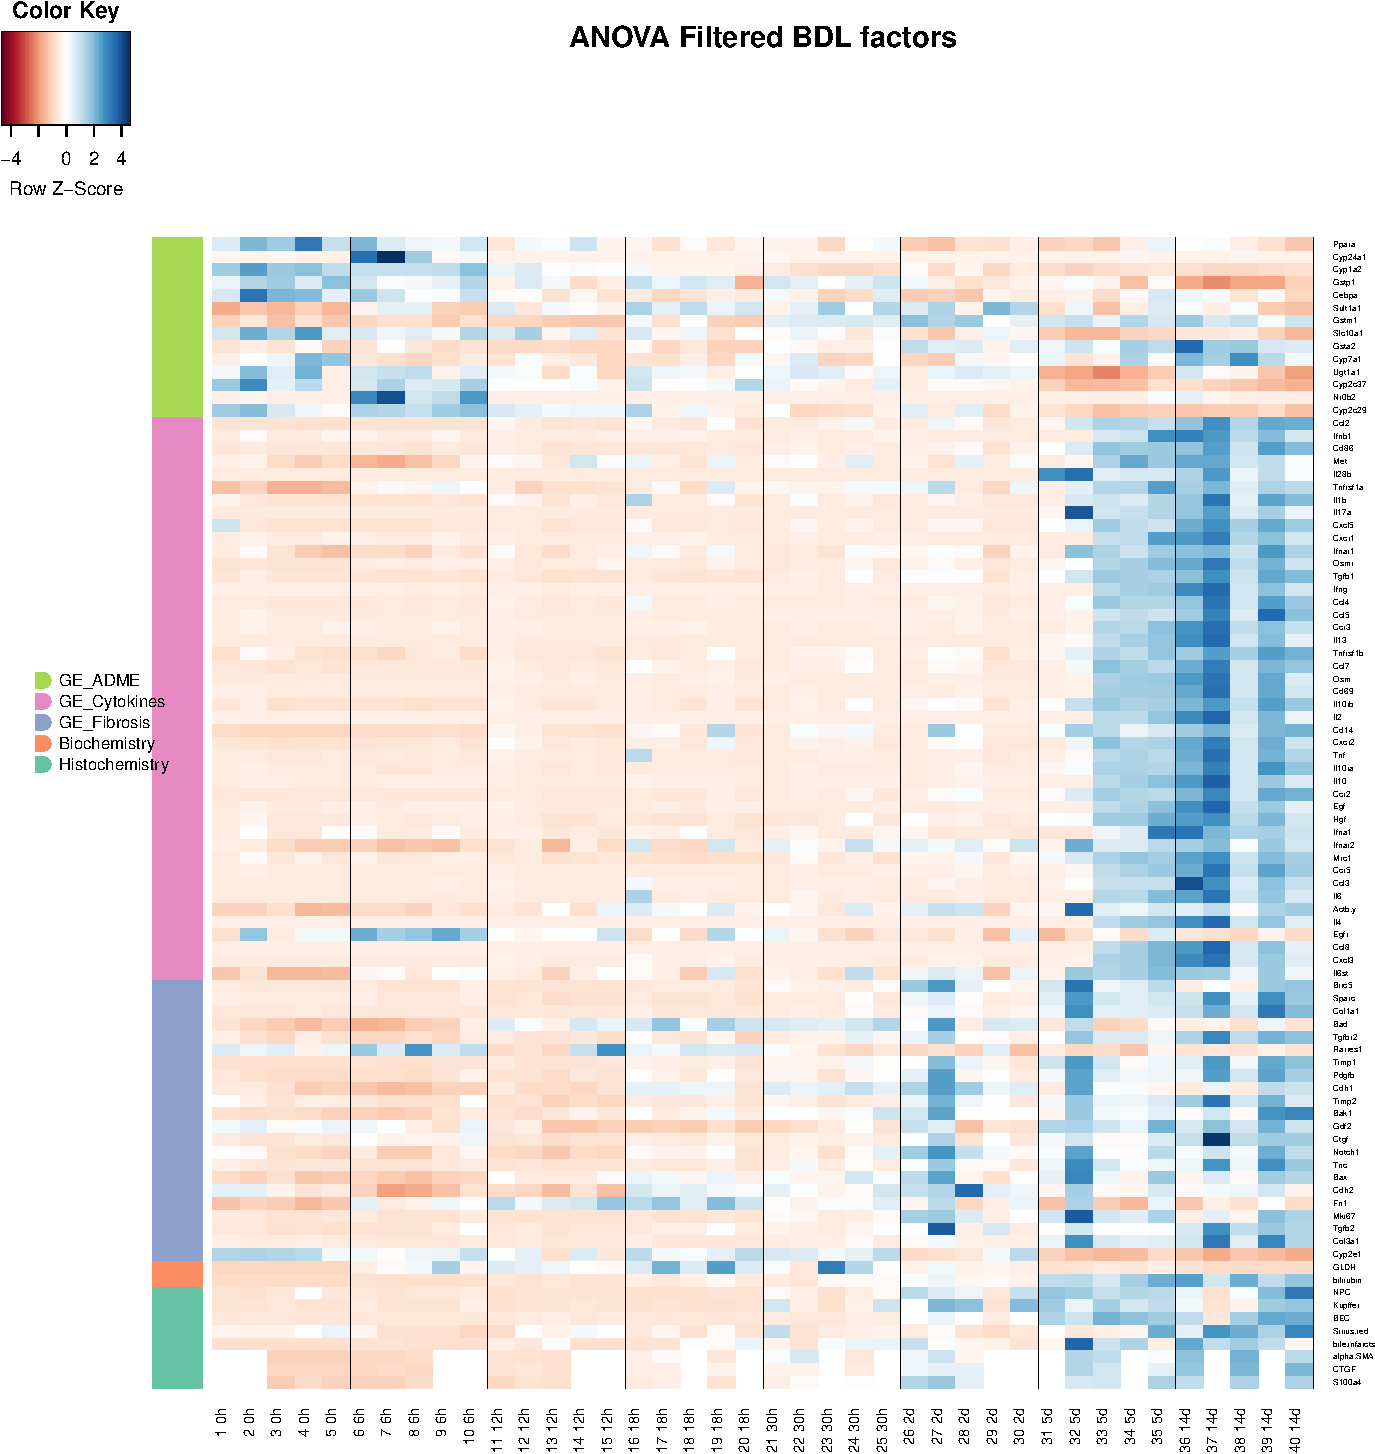
\includegraphics{Figs/heatmap_filtered_plot-1.pdf}

Figure: Filtered timecourse data. Plot of ANOVA filtered data set with
processing analog to Figure above.

\subsection{t-test for initial phase}\label{t-test-for-initial-phase}

We were in addition interested in the factors changed only in the
initial phase, i.e.~between control and the 6h time point. Therefore, a
t-test was performed to find significantly changed factors in the
initial phase after BDL.

\begin{Shaded}
\begin{Highlighting}[]
\CommentTok{# t-test for the initial phase changes}
\NormalTok{calculate_inital_phase_changes <-}\StringTok{ }\NormalTok{function()\{}
  \CommentTok{# init vectors}
  \NormalTok{p.t_test <-}\StringTok{ }\KeywordTok{rep}\NormalTok{(}\OtherTok{NA}\NormalTok{, }\KeywordTok{ncol}\NormalTok{(BDLdata))}
  \KeywordTok{names}\NormalTok{(p.t_test) <-}\StringTok{ }\KeywordTok{colnames}\NormalTok{(BDLdata)}
  \NormalTok{up_down <-}\StringTok{ }\KeywordTok{rep}\NormalTok{(}\OtherTok{NA}\NormalTok{, }\KeywordTok{ncol}\NormalTok{(BDLdata))}
  \KeywordTok{names}\NormalTok{(up_down) <-}\StringTok{ }\KeywordTok{colnames}\NormalTok{(BDLdata)}
  
  \NormalTok{for (name in }\KeywordTok{colnames}\NormalTok{(BDLdata))\{}
    \CommentTok{# data for control (0h) and initial response (6h)}
    \NormalTok{d0 <-}\StringTok{ }\NormalTok{BDLdata[BDLsamples$time_fac ==}\StringTok{ "0h"}\NormalTok{, name]}
    \NormalTok{d6 <-}\StringTok{ }\NormalTok{BDLdata[BDLsamples$time_fac ==}\StringTok{ "6h"}\NormalTok{, name]  }
    \CommentTok{# remove NA (for immunostainings Nr=3)}
    \NormalTok{d0 <-}\StringTok{ }\NormalTok{d0[!}\KeywordTok{is.na}\NormalTok{(d0)]}
    \NormalTok{d6 <-}\StringTok{ }\NormalTok{d6[!}\KeywordTok{is.na}\NormalTok{(d6)]}
    \CommentTok{# unpaired two.sided t-test}
    \NormalTok{t.test.res <-}\StringTok{ }\KeywordTok{t.test}\NormalTok{(d0, d6, }\DataTypeTok{alternative=}\StringTok{"two.sided"}\NormalTok{, }\DataTypeTok{var.equal=}\OtherTok{FALSE}\NormalTok{)}
    \NormalTok{p.t_test[name] <-}\StringTok{ }\NormalTok{t.test.res$p.value}
    \CommentTok{# going up or down}
    \NormalTok{up_down[name] <-}\StringTok{ "-"}
    \NormalTok{if (}\KeywordTok{mean}\NormalTok{(d6) >}\StringTok{ }\KeywordTok{mean}\NormalTok{(d0))\{}
      \NormalTok{up_down[name] <-}\StringTok{ "up"}
    \NormalTok{\} else if (}\KeywordTok{mean}\NormalTok{(d6) <}\StringTok{ }\KeywordTok{mean}\NormalTok{(d0))\{}
      \NormalTok{up_down[name] <-}\StringTok{ "down"}
    \NormalTok{\}}
  \NormalTok{\}}
  \CommentTok{# data.frame for t-test results}
  \NormalTok{p.df <-}\StringTok{ }\KeywordTok{data.frame}\NormalTok{(}\DataTypeTok{p.value=}\NormalTok{p.t_test, }\DataTypeTok{up_down=}\NormalTok{up_down)}
  \NormalTok{p.df$sig <-}\StringTok{ }\KeywordTok{sapply}\NormalTok{(p.df$p.value, significant_code) }
  \KeywordTok{rownames}\NormalTok{(p.df) <-}\StringTok{ }\KeywordTok{colnames}\NormalTok{(BDLdata)}
  
  \CommentTok{# sort by p.value}
  \NormalTok{p.df.ordered <-}\StringTok{ }\NormalTok{p.df[}\KeywordTok{order}\NormalTok{(p.df$p.value),]  }
  
  \KeywordTok{return}\NormalTok{(p.df.ordered)}
\NormalTok{\}}

\CommentTok{# top up and down regulated in initial phase}
\NormalTok{p.df.ordered <-}\StringTok{ }\KeywordTok{calculate_inital_phase_changes}\NormalTok{() }
\NormalTok{p.df.up <-}\StringTok{ }\NormalTok{p.df.ordered[p.df.ordered$p.value<}\FloatTok{0.05} \NormalTok{&}\StringTok{ }\NormalTok{p.df.ordered$up_down==}\StringTok{"up"}\NormalTok{, ]}
\NormalTok{p.df.down <-}\StringTok{ }\NormalTok{p.df.ordered[p.df.ordered$p.value<}\FloatTok{0.05} \NormalTok{&}\StringTok{ }\NormalTok{p.df.ordered$up_down==}\StringTok{"down"}\NormalTok{, ]}
\end{Highlighting}
\end{Shaded}

The top up- and down-regulated factors in the initial phase (independent
from the ANOVA analysis, i.e.~of all factors in data set) are \small

\begin{Shaded}
\begin{Highlighting}[]
\CommentTok{# top up}
\KeywordTok{print}\NormalTok{(p.df.up)}
\end{Highlighting}
\end{Shaded}

\begin{verbatim}
               p.value up_down sig
Tnfrsf1a  2.418075e-05      up ***
Il6st     4.777944e-04      up ***
Osmr      5.635117e-04      up ***
Fn1       2.057930e-03      up  **
Cd14      4.500421e-03      up  **
ALT       5.488831e-03      up  **
bilirubin 9.221295e-03      up  **
Nr0b2     9.693272e-03      up  **
Ctgf      1.026407e-02      up   *
Cxcl1     1.159292e-02      up   *
Timp1     1.196340e-02      up   *
Egfr      1.444607e-02      up   *
Cyp4a10   2.288889e-02      up   *
Cxcl2     2.507493e-02      up   *
GLDH      2.896681e-02      up   *
Hmox1     2.913971e-02      up   *
Socs3     3.604221e-02      up   *
Sult1a1   3.632014e-02      up   *
\end{verbatim}

\begin{Shaded}
\begin{Highlighting}[]
\CommentTok{# top down}
\KeywordTok{print}\NormalTok{(p.df.down)}
\end{Highlighting}
\end{Shaded}

\begin{verbatim}
               p.value up_down sig
Cdh2       0.005994558    down  **
Pde4a      0.010806348    down   *
Sirius.red 0.014252420    down   *
Pten       0.014853870    down   *
Col3a1     0.017104924    down   *
Nes        0.026669560    down   *
Il28b      0.027571476    down   *
Cdh1       0.027687939    down   *
Tgfb1      0.032921400    down   *
Il10ra     0.035845273    down   *
Cyp2e1     0.038398167    down   *
Cyp7a1     0.038785457    down   *
Xiap       0.041507273    down   *
\end{verbatim}

\normalsize
**Results:** In the initial phase more more up-regulations than
down-regulations are observed.

\section{Correlation analysis}\label{correlation-analysis}

For the correlation analysis between factors and the subsequent cluster
analysis a correlation measure for time series data (Son2008) in
combination with Complete-Linkage hierarchical clustering was used. This
combination of methods provided the best enrichments on gene-expression
time-series in a recent comparisons of methods (Jaskowiak2014,
Jaskowiak2013).

The calculation of correlation coefficients between factors i and j
(\(i,j=1, ...,N_p\)) was performed using the slightly modified
correlation coefficient based similarity measure developed for
clustering of time-course data. \(Y_{i,j}^{S2}\) and \(Y_{i,j}^{R2}\)
are hereby linear combinations of (i) a classical correlation part based
on Spearman correlation \(S_{i,j}^{*}\) in case of \(Y_{i,j}^{S2}\) or
Pearson \(R_{i,j}^{*}\) in case of \(Y_{i,j}^{R2}\), (ii) a component
\(A_{i,j}^{*}\) accounting for the similarity in changes between two
time courses, (iii) a component \(M_{i,j}^{*}\) comparing the location
of minimum and maximum values of the time course (see (Son2008) for
definitions)
\[Y_{i,j}^{S2} = w_1 S_{i,j}^{*} + w_2 A_{i,j}^{*} + w_3 M_{i,j}^{*}\]
\[Y_{i,j}^{R2} = w_1 R_{i,j}^{*} + w_2 A_{i,j}^{*} + w_3 M_{i,j}^{*}\]
\(R_{i,j}^{*}\) and \(S_{i,j}^{*}\) are hereby calculated on the
individual data points for the factors i and j, \(A_{i,j}^{*}\) and
\(M_{i,j}^{*}\) on the mean time courses averaged over the \(N_r\)
repeated measurements. Throughout the analysis the following weights
were used \(w_1=0.5\), \(w_2=0.3\), \(w_3=0.2\).

In the calculation of the change component we used a Spearman
correlation based measure (\(A^{**}\)) instead of the originally
proposed Pearson measure (\(A^{*}\)) resulting in the correlation scores
\(Y_{i,j}^{S3}\) and \(Y_{i,j}^{S3}\)
\[Y_{i,j}^{S3} = w_1 S_{i,j}^{*} + w_2 A_{i,j}^{**} + w_3 M_{i,j}^{*}\]
\[Y_{i,j}^{R3} = w_1 R_{i,j}^{*} + w_2 A_{i,j}^{**} + w_3 M_{i,j}^{*}\]
Herein, \(A_{i,j}^{**}\) calculates the correlation of changes between
factors i and j based on Spearman correlation analog \(A_{i,j}^{*}\) as
\[A_{i,j}^{**}=(S(d_i,d_j)+1)/2\] \[A_{i,j}^{*}=(R(d_i,d_j)+1)/2\] The
reason for this adaption was that initial analysis showed a strong
dependency of the change components on outliers.

All calculated correlation scores \(Y^{S}\) and \(Y^{R}\) are
transformed from {[}0, 1{]} to {[}-1, 1{]} via
\[Y_{norm}^{S} = 2(Y^{S}-0.5)\] \[Y_{norm}^{R} = 2(Y^{R}-0.5)\]

In addition \(Y^{S}\) and \(Y^{R}\) Pearson (R) and Spearman (S)
correlations were calculated for comparison.

\begin{Shaded}
\begin{Highlighting}[]
\KeywordTok{suppressPackageStartupMessages}\NormalTok{(}\KeywordTok{library}\NormalTok{(corrplot))}
\KeywordTok{dir.create}\NormalTok{(}\KeywordTok{file.path}\NormalTok{(resultsPath, }\StringTok{'correlation'}\NormalTok{), }\DataTypeTok{showWarnings=}\OtherTok{FALSE}\NormalTok{)}

\CommentTok{# list of calculated correlation methods}
\NormalTok{correlation_methods <-}\StringTok{ }\KeywordTok{c}\NormalTok{(}\StringTok{"pearson"}\NormalTok{, }\StringTok{"spearman"}\NormalTok{, }\StringTok{"ys1"}\NormalTok{, }\StringTok{"ys2"}\NormalTok{, }\StringTok{"ys3"}\NormalTok{, }\StringTok{"yr1"}\NormalTok{, }\StringTok{"yr2"}\NormalTok{, }\StringTok{"yr3"}\NormalTok{)}

\CommentTok{# calculated correlation matrices are stored in cor.matrices}
\NormalTok{cor.matrices <-}\StringTok{ }\KeywordTok{vector}\NormalTok{(}\StringTok{"list"}\NormalTok{, }\DataTypeTok{length=}\KeywordTok{length}\NormalTok{(correlation_methods))}
\KeywordTok{names}\NormalTok{(cor.matrices) <-}\StringTok{ }\NormalTok{correlation_methods}
\end{Highlighting}
\end{Shaded}

\subsection{Pearson \& Spearman
correlation}\label{pearson-spearman-correlation}

To get an overview over the correlation structure of the data set, we
first calculated Pearson \(R_{i,j}\) and Spearman \(S_{i,j}\)
correlation were calculated for the subset of filtered factors.

\begin{Shaded}
\begin{Highlighting}[]
\CommentTok{# Spearman and Pearson on individual data points}
\NormalTok{cor.matrices$pearson <-}\StringTok{ }\KeywordTok{cor}\NormalTok{(BDLdata.fil, }\DataTypeTok{method=}\StringTok{"pearson"}\NormalTok{, }\DataTypeTok{use=}\StringTok{"pairwise.complete.obs"}\NormalTok{)}
\NormalTok{cor.matrices$spearman <-}\StringTok{ }\KeywordTok{cor}\NormalTok{(BDLdata.fil, }\DataTypeTok{method=}\StringTok{"spearman"}\NormalTok{, }\DataTypeTok{use=}\StringTok{"pairwise.complete.obs"}\NormalTok{)}
\end{Highlighting}
\end{Shaded}

Heatmap plot of the correlation matrices with factors in original order

\begin{Shaded}
\begin{Highlighting}[]
\CommentTok{# Heatmap of correlation matrix}
\NormalTok{correlation_heatmap <-}\StringTok{ }\NormalTok{function(method)\{}
  \NormalTok{data <-}\StringTok{ }\NormalTok{cor.matrices[[method]]}
  \NormalTok{if(}\KeywordTok{is.null}\NormalTok{(data))\{}
    \KeywordTok{stop}\NormalTok{(}\StringTok{"Correlation matrix does not exist for method: "}\NormalTok{, method)}
  \NormalTok{\}}
  \NormalTok{cor_colors <-}\StringTok{ }\KeywordTok{HeatmapColors}\NormalTok{() }\CommentTok{# color palette for correlation (red - white - blue)}
  \KeywordTok{heatmap.2}\NormalTok{(data, }\DataTypeTok{col=}\KeywordTok{cor_colors}\NormalTok{(}\DecValTok{10}\NormalTok{), }\DataTypeTok{scale=}\StringTok{"none"}\NormalTok{,}
          \DataTypeTok{key=}\OtherTok{TRUE}\NormalTok{, }\DataTypeTok{symkey=}\OtherTok{FALSE}\NormalTok{, }\DataTypeTok{trace=}\StringTok{"none"}\NormalTok{, }\DataTypeTok{cexRow=}\FloatTok{0.8}\NormalTok{, }\DataTypeTok{cexCol=}\FloatTok{0.8}\NormalTok{,}
          \DataTypeTok{main=}\NormalTok{method,}
          \DataTypeTok{density.info=}\StringTok{"none"}\NormalTok{, }\DataTypeTok{dendrogram=}\StringTok{"none"}\NormalTok{, }
          \DataTypeTok{Rowv=}\OtherTok{NULL}\NormalTok{, }\DataTypeTok{Colv=}\OtherTok{NULL}\NormalTok{, }
          \DataTypeTok{keysize=}\FloatTok{0.8}\NormalTok{, }\DataTypeTok{key.xlab =} \NormalTok{method,}
          \CommentTok{#revC=TRUE,}
          \DataTypeTok{sepwidth=}\KeywordTok{c}\NormalTok{(}\FloatTok{0.01}\NormalTok{,}\FloatTok{0.01}\NormalTok{),}
          \DataTypeTok{sepcolor=}\StringTok{"black"}\NormalTok{,}
          \DataTypeTok{colsep=}\DecValTok{1}\NormalTok{:}\KeywordTok{ncol}\NormalTok{(data),}
          \DataTypeTok{rowsep=}\DecValTok{1}\NormalTok{:}\KeywordTok{nrow}\NormalTok{(data))}
\NormalTok{\}}
\end{Highlighting}
\end{Shaded}

\begin{Shaded}
\begin{Highlighting}[]
\CommentTok{# Pearson correlation (no clustering)}
\KeywordTok{correlation_heatmap}\NormalTok{(}\DataTypeTok{method=}\StringTok{"pearson"}\NormalTok{)}
\end{Highlighting}
\end{Shaded}

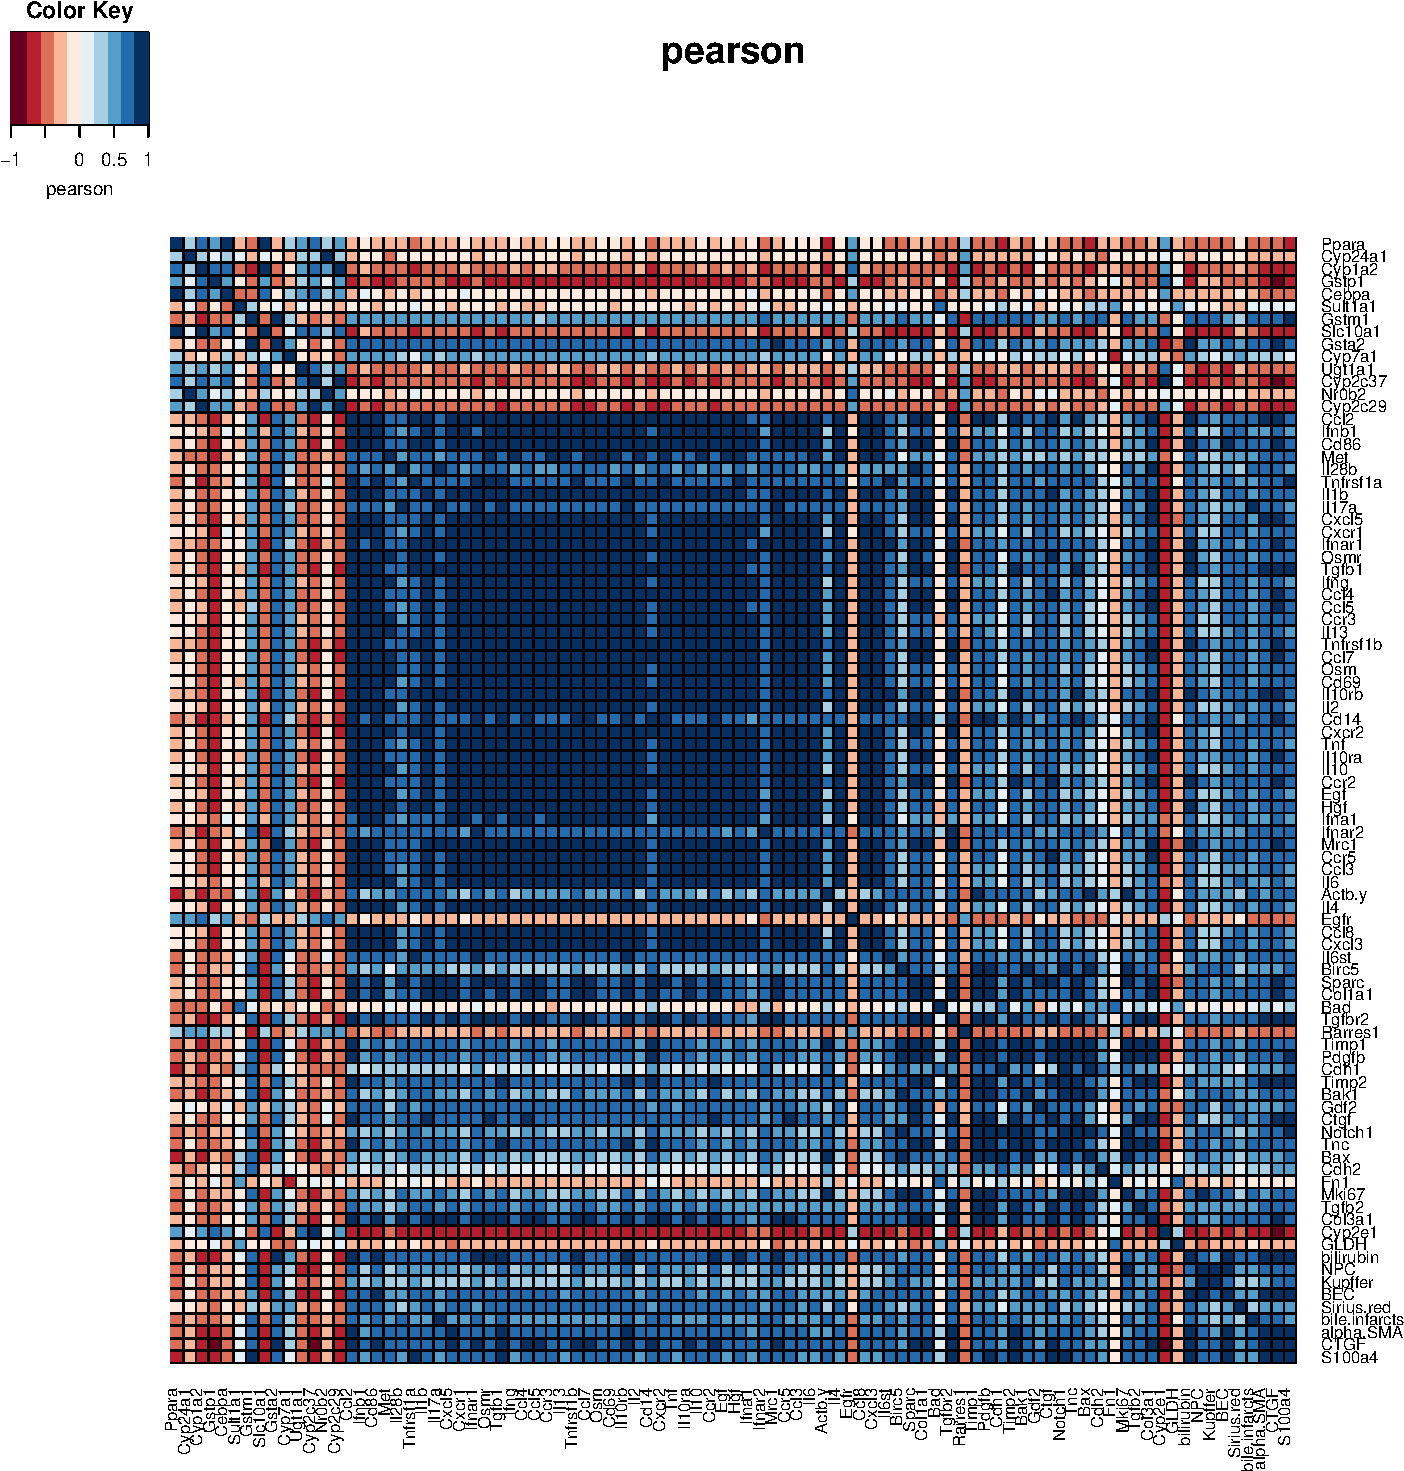
\includegraphics{Figs/heatmap_pearson-1.pdf}

Figure: Heatmap of Pearson correlation. Correlation matrix based on
Pearson correlation for filtered data set. No clustering was applied.

\begin{Shaded}
\begin{Highlighting}[]
\CommentTok{# Spearman correlation (no clustering)}
\KeywordTok{correlation_heatmap}\NormalTok{(}\DataTypeTok{method=}\StringTok{"spearman"}\NormalTok{)}
\end{Highlighting}
\end{Shaded}

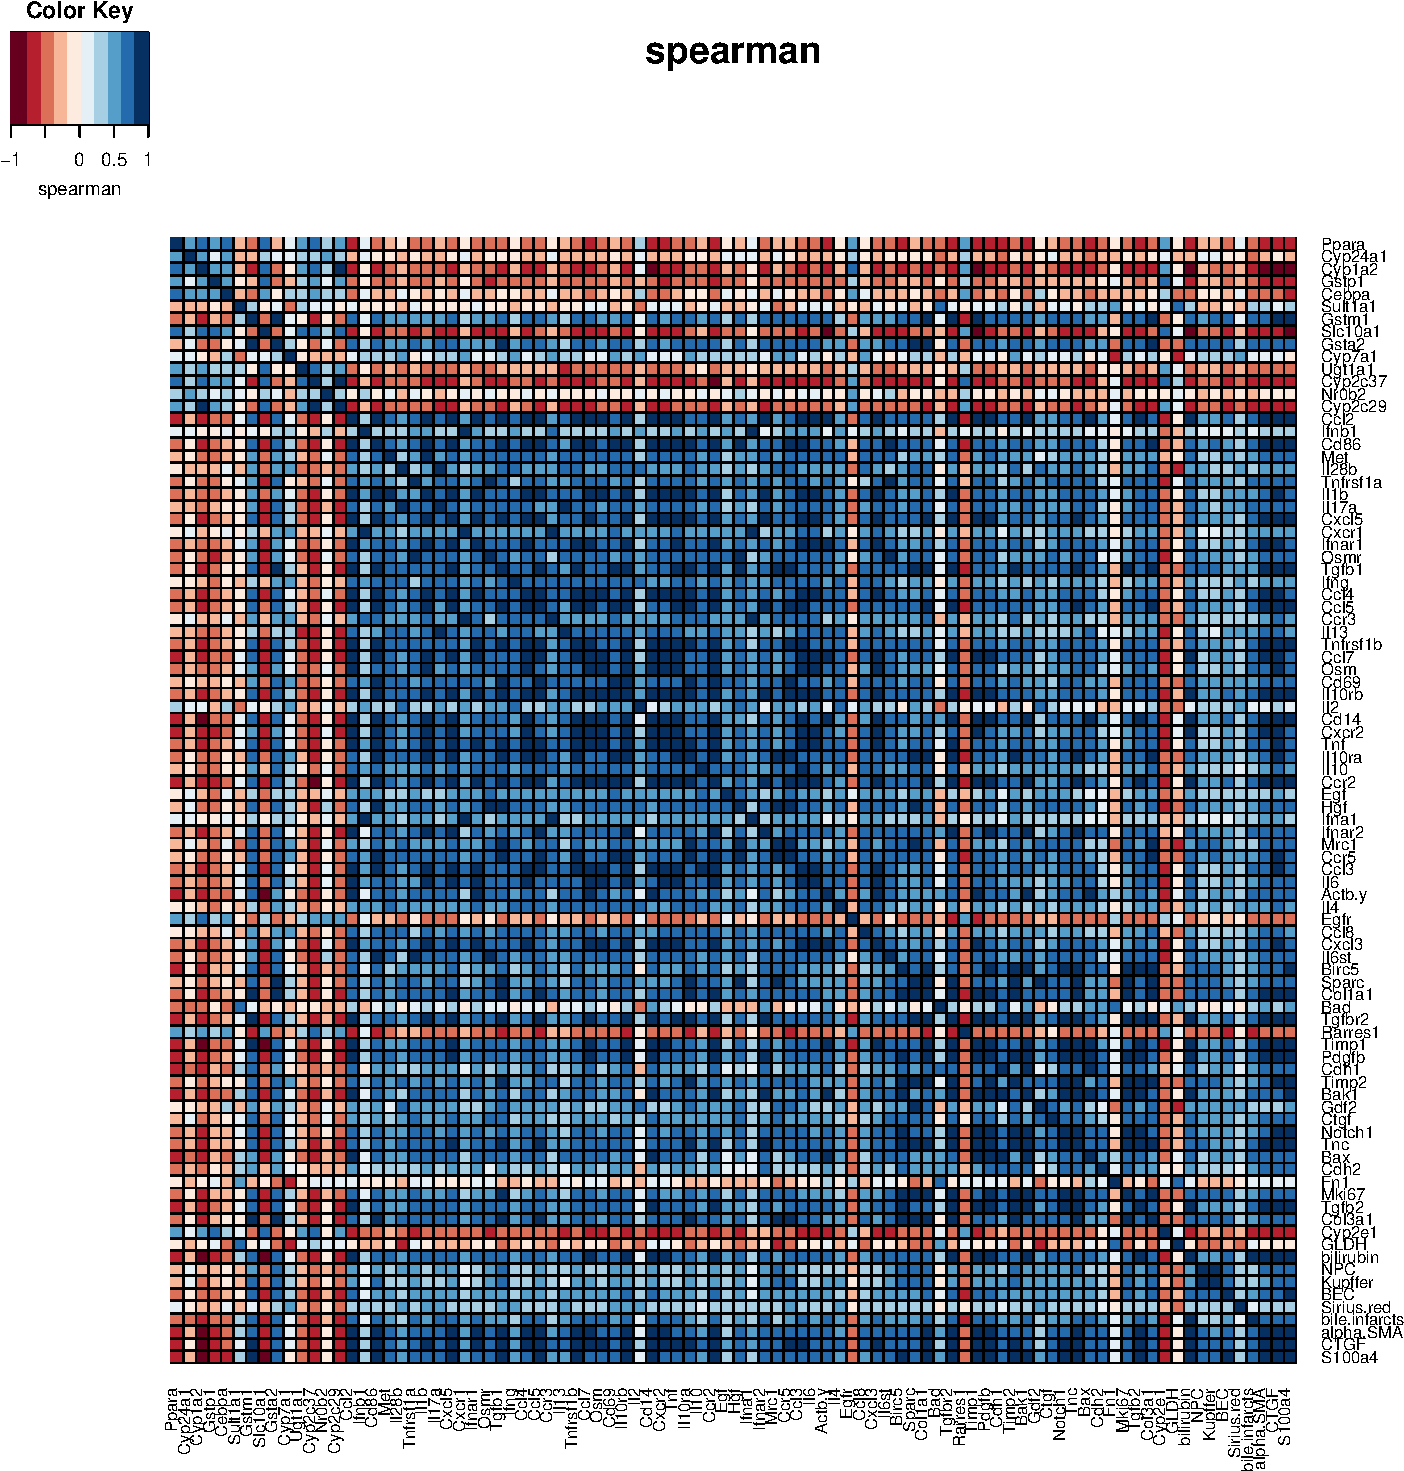
\includegraphics{Figs/heatmap_spearman-1.pdf}

Figure: Heatmap of Spearman correlation. Correlation matrix based on
Spearman correlation for filtered data set. No clustering was applied.

\textbf{Results:} The general correlation structure is similar between
Pearson and Spearman, but the pearson correlation showed much more
sensitive to outliers resulting in a large block of very high correlated
factors. Spearman based correlatino coped much better with these
outliers. Prelimary analysis of \(A^{*}\) showed similar problems, so we
used \(A^{**}\) in \(Y^{S3}\) instead.

\subsection{YS \& YR correlation}\label{ys-yr-correlation}

Now the time-course based correlation measurements \(Y^{S1}\),
\(Y^{S2}\), \(Y^{S3}\), \(Y^{R1}\), \(Y^{R2}\) and \(Y^{R3}\) are
calculated for all factors in the filtered data set. For the calculation
of the correlation matrix all pairwise correlations between the factors
were calculated. In the later analysis only the outlier robust
\(Y^{S3}\) is used.

\begin{Shaded}
\begin{Highlighting}[]
\CommentTok{# weighting factors}
\NormalTok{w <-}\StringTok{ }\KeywordTok{list}\NormalTok{(}\DataTypeTok{w1=}\FloatTok{0.5}\NormalTok{, }\DataTypeTok{w2=}\FloatTok{0.3}\NormalTok{, }\DataTypeTok{w3=}\FloatTok{0.2}\NormalTok{)}

\CommentTok{# calculate the YSR component matrices on the filtered data set (A, A*, A**, M, M*)}
\CommentTok{# all components are calculated on the mean data}
\NormalTok{ysr.res <-}\StringTok{ }\KeywordTok{ysr.matrices}\NormalTok{(BDLmean.fil, BDLmean.time, }\DataTypeTok{use=}\StringTok{"pairwise.complete.obs"}\NormalTok{)}

\CommentTok{# S* and R* (Pearson & Spearman correlation on individual data points)}
\NormalTok{cor.S_star <-}\StringTok{ }\NormalTok{(cor.matrices$spearman +}\StringTok{ }\DecValTok{1}\NormalTok{)/}\DecValTok{2}
\NormalTok{cor.R_star <-}\StringTok{ }\NormalTok{(cor.matrices$pearson +}\StringTok{ }\DecValTok{1}\NormalTok{)/}\DecValTok{2}

\CommentTok{# Calculate YS and YR scores based on the components}
\NormalTok{ysr_methods <-}\StringTok{ }\KeywordTok{c}\NormalTok{(}\StringTok{"ys1"}\NormalTok{, }\StringTok{"ys2"}\NormalTok{, }\StringTok{"ys3"}\NormalTok{, }\StringTok{"yr1"}\NormalTok{, }\StringTok{"yr2"}\NormalTok{, }\StringTok{"yr3"}\NormalTok{)}
\NormalTok{cor.ysr <-}\StringTok{ }\KeywordTok{vector}\NormalTok{(}\StringTok{"list"}\NormalTok{, }\KeywordTok{length}\NormalTok{(ysr_methods))}
\KeywordTok{names}\NormalTok{(cor.ysr) <-}\StringTok{ }\NormalTok{ysr_methods}

\CommentTok{# unnormalized correlations in [0, 1] as combination of weighted (S/R, A/A*/A**, M/M*)}
\NormalTok{cor.ysr$ys1 <-}\StringTok{ }\NormalTok{w$w1*cor.S_star +}\StringTok{ }\NormalTok{w$w2*ysr.res$A       +}\StringTok{ }\NormalTok{w$w3*ysr.res$M}
\NormalTok{cor.ysr$ys2 <-}\StringTok{ }\NormalTok{w$w1*cor.S_star +}\StringTok{ }\NormalTok{w$w2*ysr.res$A_star  +}\StringTok{ }\NormalTok{w$w3*ysr.res$M_star}
\NormalTok{cor.ysr$ys3 <-}\StringTok{ }\NormalTok{w$w1*cor.S_star +}\StringTok{ }\NormalTok{w$w2*ysr.res$A_star2 +}\StringTok{ }\NormalTok{w$w3*ysr.res$M_star}

\NormalTok{cor.ysr$yr1 <-}\StringTok{ }\NormalTok{w$w1*cor.R_star +}\StringTok{ }\NormalTok{w$w2*ysr.res$A       +}\StringTok{ }\NormalTok{w$w3*ysr.res$M}
\NormalTok{cor.ysr$yr2 <-}\StringTok{ }\NormalTok{w$w1*cor.R_star +}\StringTok{ }\NormalTok{w$w2*ysr.res$A_star  +}\StringTok{ }\NormalTok{w$w3*ysr.res$M_star}
\NormalTok{cor.ysr$yr3 <-}\StringTok{ }\NormalTok{w$w1*cor.R_star +}\StringTok{ }\NormalTok{w$w2*ysr.res$A_star2 +}\StringTok{ }\NormalTok{w$w3*ysr.res$M_star }

\CommentTok{# scaling of ysr correlation coefficient to interval [-1,1]}
\NormalTok{for (method in ysr_methods)\{}
  \NormalTok{cor.matrices[[method]] <-}\StringTok{ }\DecValTok{2}\NormalTok{*(cor.ysr[[method]]-}\FloatTok{0.5}\NormalTok{)}
\NormalTok{\}}

\CommentTok{# Save correlation matrices}
\KeywordTok{save}\NormalTok{(cor.matrices, }\DataTypeTok{file=}\KeywordTok{file.path}\NormalTok{(resultsPath, }\StringTok{"data"}\NormalTok{, }\StringTok{"cor.matrices.Rdata"}\NormalTok{))}
\KeywordTok{rm}\NormalTok{(cor.ysr, cor.R_star, cor.S_star, ysr.res, ysr_methods)}
\end{Highlighting}
\end{Shaded}

Create heatmap plots for all calculated correlation matrices

\begin{Shaded}
\begin{Highlighting}[]
\CommentTok{# create all correlation heatmaps on disk}
\NormalTok{hmap.settings <-}\StringTok{ }\KeywordTok{list}\NormalTok{(}\DataTypeTok{width=}\DecValTok{10}\NormalTok{, }\DataTypeTok{height=}\DecValTok{10}\NormalTok{, }\DataTypeTok{pointsize=}\DecValTok{12}\NormalTok{)}
\NormalTok{for (method in correlation_methods)\{}
  \NormalTok{fname <-}\StringTok{ }\KeywordTok{sprintf}\NormalTok{(}\StringTok{'cor.%s.pdf'}\NormalTok{, method)}
  \KeywordTok{pdf}\NormalTok{(}\KeywordTok{file.path}\NormalTok{(resultsPath, }\StringTok{"correlation"}\NormalTok{, fname),}
      \DataTypeTok{width=}\NormalTok{hmap.settings$width, }\DataTypeTok{height=}\NormalTok{hmap.settings$height, }
      \DataTypeTok{pointsize=}\NormalTok{hmap.settings$pointsize)}
  \KeywordTok{correlation_heatmap}\NormalTok{(}\DataTypeTok{method=}\NormalTok{method)}
\KeywordTok{invisible}\NormalTok{(}\KeywordTok{dev.off}\NormalTok{())}
\KeywordTok{rm}\NormalTok{(method, fname)}
\NormalTok{\}}
\end{Highlighting}
\end{Shaded}

\begin{Shaded}
\begin{Highlighting}[]
\CommentTok{# ys3 heatmap in report}
\KeywordTok{correlation_heatmap}\NormalTok{(}\DataTypeTok{method=}\StringTok{"ys3"}\NormalTok{)}
\end{Highlighting}
\end{Shaded}

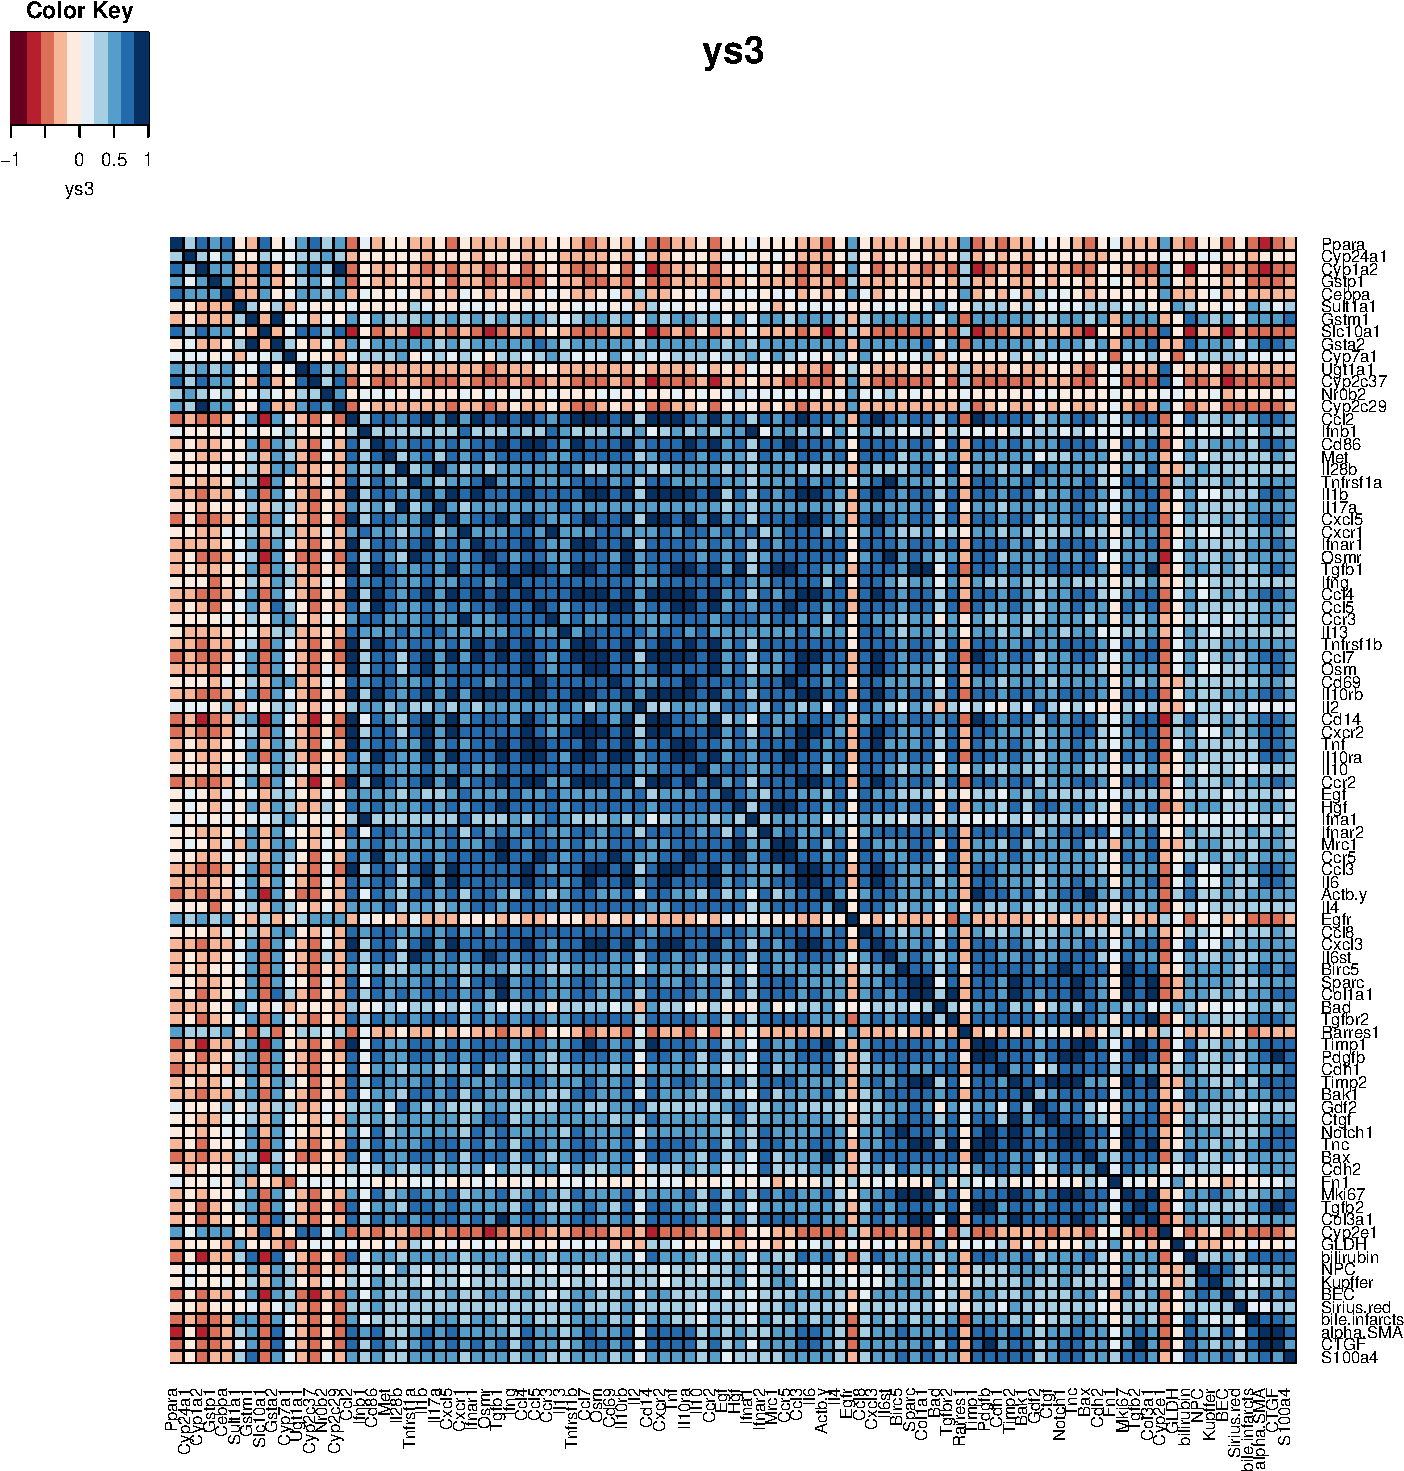
\includegraphics{Figs/ys3_correlation_report-1.pdf}

Figure: Heatmap of YS3 correlation. Correlation matrix based on YS3
correlation for filtered data set. No clustering was applied.

\section{Hierarchical clustering}\label{hierarchical-clustering}

\subsection{Clustering}\label{clustering}

Now clusters are calculated based on the calculated correlation matrices
using hierarchical clustering with complete linkage. Hereby, the factors
are grouped into a number of clusters with the correlation within each
cluster being larger than between clusters. For a time course based
correlation measure like \(Y^{S3}\) this effectivly finds groups of
factors which have similar time courses. The complete linkage method
defines the cluster distance between two clusters to be the maximum
distance between their individual components.

The resulting hierarchical clustering based on the given correlation
matrix is split into \texttt{Ngroups=6} clusters (prelimenary analysis
showed that a higher number of clusters results in clusters with only
one member). The number of clusters was choosen, so that at least
\texttt{\textgreater{}1} members exist per cluster.

\begin{Shaded}
\begin{Highlighting}[]
\NormalTok{hclust.res <-}\StringTok{ }\KeywordTok{vector}\NormalTok{(}\StringTok{"list"}\NormalTok{, }\DataTypeTok{length=}\KeywordTok{length}\NormalTok{(correlation_methods))}
\KeywordTok{names}\NormalTok{(hclust.res) <-}\StringTok{ }\NormalTok{correlation_methods}

\CommentTok{# Calculate hierarical clustering: N clusters for correlation based on method}
\NormalTok{calculate_clusters <-}\StringTok{ }\NormalTok{function(cor_method, N)\{}
  \CommentTok{# get correlation matrix}
  \NormalTok{cor.cluster <-}\StringTok{ }\NormalTok{cor.matrices[[cor_method]]}
  \CommentTok{# perform hierarchical clustering (complete linkage & Euclidion distance measure)}
  \NormalTok{hc <-}\StringTok{ }\KeywordTok{hclust}\NormalTok{(}\KeywordTok{dist}\NormalTok{(cor.cluster, }\DataTypeTok{method=}\StringTok{"euclidian"}\NormalTok{), }\DataTypeTok{method=}\StringTok{"complete"}\NormalTok{) }
  \CommentTok{# cut into the clusters}
  \NormalTok{groups <-}\StringTok{ }\KeywordTok{cutree}\NormalTok{(hc, }\DataTypeTok{k=}\NormalTok{Ngroups)}
  \NormalTok{groups.hc.order <-}\StringTok{ }\NormalTok{groups[hc$order]}
  \CommentTok{# store results}
  \KeywordTok{return}\NormalTok{(}\KeywordTok{list}\NormalTok{(}\DataTypeTok{hc=}\NormalTok{hc,}
              \DataTypeTok{groups=}\NormalTok{groups,}
              \DataTypeTok{groups.hc.order=}\NormalTok{groups.hc.order))}
\NormalTok{\}}

\NormalTok{Ngroups <-}\StringTok{ }\DecValTok{6}   \CommentTok{# number of clusters}
\NormalTok{for (method in correlation_methods)\{}
  \NormalTok{hclust.res[[method]] <-}\StringTok{ }\KeywordTok{calculate_clusters}\NormalTok{(}\DataTypeTok{cor_method=}\NormalTok{method, }\DataTypeTok{N=}\NormalTok{Ngroups)}
\NormalTok{\}}
\CommentTok{# save clustering}
\KeywordTok{save}\NormalTok{(hclust.res, }\DataTypeTok{file=}\KeywordTok{file.path}\NormalTok{(resultsPath, }\StringTok{"data"}\NormalTok{, }\StringTok{"hclust.res.Rdata"}\NormalTok{))}
\KeywordTok{rm}\NormalTok{(method)}
\end{Highlighting}
\end{Shaded}

In the next step the correlation matrices are plotted in combination
with the clustering results (dendrogram) and the clusters as side
colors.

\begin{Shaded}
\begin{Highlighting}[]
\CommentTok{# Create correlation heatmap with hierachical clustering results}
\NormalTok{correlation_heatmap_cluster <-}\StringTok{ }\NormalTok{function(method)\{}
  \CommentTok{# matrix and cluster results}
  \NormalTok{cor.cluster <-}\StringTok{ }\NormalTok{cor.matrices[[method]]}
  \NormalTok{hc.res <-}\StringTok{ }\NormalTok{hclust.res[[method]]}
  \NormalTok{hc <-}\StringTok{ }\NormalTok{hc.res$hc}
  \NormalTok{groups <-}\StringTok{ }\NormalTok{hc.res$groups}
  \CommentTok{# colors}
  \NormalTok{hmap_colors <-}\StringTok{ }\KeywordTok{HeatmapColors}\NormalTok{()}
  \NormalTok{colorset <-}\StringTok{ }\KeywordTok{brewer.pal}\NormalTok{(Ngroups, }\StringTok{"Set1"}\NormalTok{)}
  \NormalTok{color.map <-}\StringTok{ }\NormalTok{function(cluster_id) \{}\KeywordTok{return}\NormalTok{(colorset[cluster_id])\}}
  \NormalTok{clusterColors <-}\StringTok{ }\KeywordTok{unlist}\NormalTok{(}\KeywordTok{lapply}\NormalTok{(groups, color.map))}
  
  \KeywordTok{heatmap.2}\NormalTok{(cor.cluster, }\DataTypeTok{col=}\KeywordTok{hmap_colors}\NormalTok{(}\DecValTok{10}\NormalTok{), }\DataTypeTok{scale=}\StringTok{"none"}\NormalTok{,}
          \DataTypeTok{key=}\OtherTok{TRUE}\NormalTok{, }\DataTypeTok{symkey=}\OtherTok{FALSE}\NormalTok{, }\DataTypeTok{trace=}\StringTok{"none"}\NormalTok{, }\DataTypeTok{cexRow=}\FloatTok{0.8}\NormalTok{, }\DataTypeTok{cexCol=}\FloatTok{0.8}\NormalTok{,}
          \DataTypeTok{main=}\NormalTok{method,}
          \DataTypeTok{density.info=}\StringTok{"none"}\NormalTok{, }\DataTypeTok{dendrogram=}\StringTok{"column"}\NormalTok{, }
          \DataTypeTok{Rowv=}\KeywordTok{as.dendrogram}\NormalTok{(hc), }\DataTypeTok{Colv=}\KeywordTok{as.dendrogram}\NormalTok{(hc), }
          \DataTypeTok{keysize=}\FloatTok{0.8}\NormalTok{,}
          \DataTypeTok{key.xlab=}\NormalTok{method,}
          \DataTypeTok{ColSideColors=}\NormalTok{clusterColors, }\DataTypeTok{revC=}\OtherTok{TRUE}\NormalTok{,}
          \DataTypeTok{sepwidth=}\KeywordTok{c}\NormalTok{(}\FloatTok{0.01}\NormalTok{,}\FloatTok{0.01}\NormalTok{),}
          \DataTypeTok{sepcolor=}\StringTok{"black"}\NormalTok{,}
          \DataTypeTok{colsep=}\DecValTok{1}\NormalTok{:}\KeywordTok{ncol}\NormalTok{(cor.cluster),}
          \DataTypeTok{rowsep=}\DecValTok{1}\NormalTok{:}\KeywordTok{nrow}\NormalTok{(cor.cluster),}
          \DataTypeTok{margins=}\KeywordTok{c}\NormalTok{(}\DecValTok{12}\NormalTok{,}\DecValTok{8}\NormalTok{))}
  \KeywordTok{legend}\NormalTok{(}\StringTok{"left"}\NormalTok{, }\DataTypeTok{legend=}\KeywordTok{paste}\NormalTok{(}\StringTok{"c"}\NormalTok{, }\DecValTok{1}\NormalTok{:}\DecValTok{6}\NormalTok{, }\DataTypeTok{sep=}\StringTok{""}\NormalTok{), }
         \DataTypeTok{col=} \KeywordTok{unlist}\NormalTok{(}\KeywordTok{lapply}\NormalTok{(}\DecValTok{1}\NormalTok{:}\DecValTok{6}\NormalTok{, color.map)), }\DataTypeTok{pch=}\DecValTok{15}\NormalTok{, }\DataTypeTok{bty=}\StringTok{"n"}\NormalTok{)}
\NormalTok{\}}

\CommentTok{# plot to files}
\NormalTok{for(method in correlation_methods)\{}
  \KeywordTok{pdf}\NormalTok{(}\KeywordTok{file.path}\NormalTok{(resultsPath, }\StringTok{"correlation"}\NormalTok{, }\KeywordTok{sprintf}\NormalTok{(}\StringTok{"cor.%s.hclust.pdf"}\NormalTok{, method)), }
      \DataTypeTok{width=}\DecValTok{10}\NormalTok{, }\DataTypeTok{height=}\DecValTok{10}\NormalTok{, }\DataTypeTok{pointsize=}\DecValTok{12}\NormalTok{) }
  \KeywordTok{correlation_heatmap_cluster}\NormalTok{(}\DataTypeTok{method=}\NormalTok{method)}
  \KeywordTok{invisible}\NormalTok{(}\KeywordTok{dev.off}\NormalTok{())  }
\NormalTok{\}}
\KeywordTok{rm}\NormalTok{(method)}
\end{Highlighting}
\end{Shaded}

\begin{Shaded}
\begin{Highlighting}[]
\CommentTok{# plot ys3 clustering to report}
\KeywordTok{correlation_heatmap_cluster}\NormalTok{(}\DataTypeTok{method=}\StringTok{"ys3"}\NormalTok{)}
\end{Highlighting}
\end{Shaded}

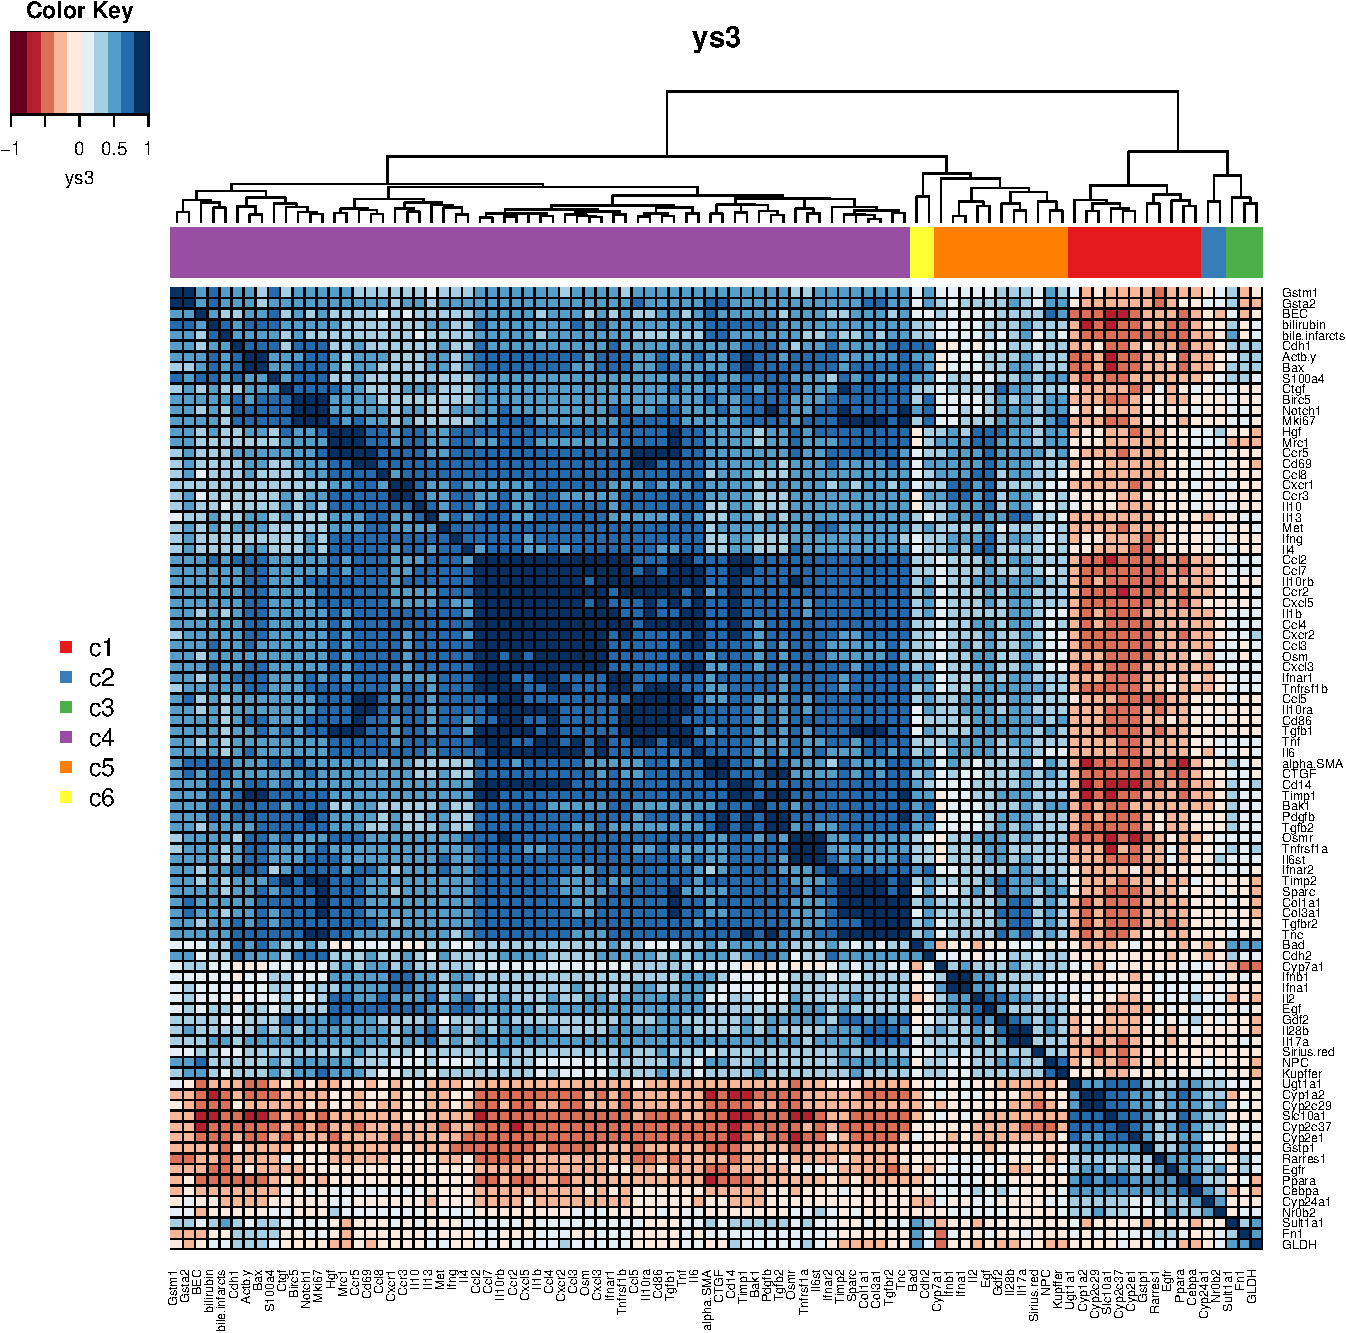
\includegraphics{Figs/heatmap_ys3-1.pdf}

Figure: Heatmap of YS3 clustering. Correlation matrix based on YS3
correlation for filtered data set with hierarchical clustering results
based on complete linkage.

The following factors are in the \texttt{ys3} time course clusters.

\begin{Shaded}
\begin{Highlighting}[]
\CommentTok{# print representatives of cluster}
\NormalTok{list_cluster_members <-}\StringTok{ }\NormalTok{function(method)\{}
  \NormalTok{groups <-}\StringTok{ }\NormalTok{hclust.res[[method]]$groups}
  \KeywordTok{cat}\NormalTok{(}\KeywordTok{sprintf}\NormalTok{(}\StringTok{"------------------------------------------}\CharTok{\textbackslash{}n}\StringTok{"}\NormalTok{))}
  \KeywordTok{cat}\NormalTok{(}\KeywordTok{sprintf}\NormalTok{(}\StringTok{"Correlation method: *** %s ***}\CharTok{\textbackslash{}n}\StringTok{"}\NormalTok{, method))}
  \KeywordTok{cat}\NormalTok{(}\KeywordTok{sprintf}\NormalTok{(}\StringTok{"------------------------------------------}\CharTok{\textbackslash{}n}\StringTok{"}\NormalTok{))}
  \NormalTok{for (k in }\DecValTok{1}\NormalTok{:Ngroups)\{}
    \NormalTok{g <-}\StringTok{ }\NormalTok{groups[groups==k]}
    \KeywordTok{cat}\NormalTok{(}\KeywordTok{sprintf}\NormalTok{(}\StringTok{"Cluster %s (N=%s)}\CharTok{\textbackslash{}n}\StringTok{"}\NormalTok{, k, }\KeywordTok{length}\NormalTok{(g)))}
    \KeywordTok{print}\NormalTok{(}\KeywordTok{names}\NormalTok{(g))}
    \KeywordTok{cat}\NormalTok{(}\StringTok{"}\CharTok{\textbackslash{}n}\StringTok{"}\NormalTok{)}
    \CommentTok{# print(paste(names(g), sep=", ", collapse =", " ))}
  \NormalTok{\}  }
\NormalTok{\}}
\end{Highlighting}
\end{Shaded}

\small

\begin{Shaded}
\begin{Highlighting}[]
\KeywordTok{list_cluster_members}\NormalTok{(}\DataTypeTok{method=}\StringTok{"ys3"}\NormalTok{)}
\end{Highlighting}
\end{Shaded}

\begin{verbatim}
------------------------------------------
Correlation method: *** ys3 ***
------------------------------------------
Cluster 1 (N=11)
 [1] "Ppara"   "Cyp1a2"  "Gstp1"   "Cebpa"   "Slc10a1" "Ugt1a1"  "Cyp2c37"
 [8] "Cyp2c29" "Egfr"    "Rarres1" "Cyp2e1" 

Cluster 2 (N=2)
[1] "Cyp24a1" "Nr0b2"  

Cluster 3 (N=3)
[1] "Sult1a1" "Fn1"     "GLDH"   

Cluster 4 (N=61)
 [1] "Gstm1"         "Gsta2"         "Ccl2"          "Cd86"         
 [5] "Met"           "Tnfrsf1a"      "Il1b"          "Cxcl5"        
 [9] "Cxcr1"         "Ifnar1"        "Osmr"          "Tgfb1"        
[13] "Ifng"          "Ccl4"          "Ccl5"          "Ccr3"         
[17] "Il13"          "Tnfrsf1b"      "Ccl7"          "Osm"          
[21] "Cd69"          "Il10rb"        "Cd14"          "Cxcr2"        
[25] "Tnf"           "Il10ra"        "Il10"          "Ccr2"         
[29] "Hgf"           "Ifnar2"        "Mrc1"          "Ccr5"         
[33] "Ccl3"          "Il6"           "Actb.y"        "Il4"          
[37] "Ccl8"          "Cxcl3"         "Il6st"         "Birc5"        
[41] "Sparc"         "Col1a1"        "Tgfbr2"        "Timp1"        
[45] "Pdgfb"         "Cdh1"          "Timp2"         "Bak1"         
[49] "Ctgf"          "Notch1"        "Tnc"           "Bax"          
[53] "Mki67"         "Tgfb2"         "Col3a1"        "bilirubin"    
[57] "BEC"           "bile.infarcts" "alpha.SMA"     "CTGF"         
[61] "S100a4"       

Cluster 5 (N=11)
 [1] "Cyp7a1"     "Ifnb1"      "Il28b"      "Il17a"      "Il2"       
 [6] "Egf"        "Ifna1"      "Gdf2"       "NPC"        "Kupffer"   
[11] "Sirius.red"

Cluster 6 (N=2)
[1] "Bad"  "Cdh2"
\end{verbatim}

\normalsize

\subsection{Correlations for non-transcript
factors}\label{correlations-for-non-transcript-factors}

In the following steps we look at specific parts of the correlation
matrix. First we are interested in the correlations between transcripts
and classical factors, i.e.~biochemical and (immuno-)histochemical
factors. The genes are filtered based on a cutoff for the correlation,
i.e.~columns in which no correlation coefficient
\texttt{abs(value) \textgreater{}= cor.cutoff} exists are filtered out.
Consequently, only transcripts are retained with a absolute correlation
coeffient above this threshold.

\begin{Shaded}
\begin{Highlighting}[]
\NormalTok{get_histological_correlations <-}\StringTok{ }\NormalTok{function(}\DataTypeTok{method=}\StringTok{"ys3"}\NormalTok{, }\DataTypeTok{cor.cutoff=}\FloatTok{0.6}\NormalTok{)\{}
  \CommentTok{# correlation matrix}
  \NormalTok{cor_mat <-}\StringTok{ }\NormalTok{cor.matrices[[method]]}
  
  \CommentTok{# non-transcipt factors accepted by ANOVA}
  \NormalTok{hist_facs <-}\StringTok{ }\NormalTok{BDLfactors$id[anova.accept &}\StringTok{ }
\StringTok{                }\NormalTok{(BDLfactors$ftype %in%}\StringTok{ }\KeywordTok{c}\NormalTok{(}\StringTok{"Biochemistry"}\NormalTok{, }\StringTok{"Histochemistry"}\NormalTok{))]}
  
  \CommentTok{# get indices of these factors in correlation matrix}
  \NormalTok{hist_idx <-}\StringTok{ }\KeywordTok{rep}\NormalTok{(}\OtherTok{NA}\NormalTok{, }\KeywordTok{length}\NormalTok{(hist_facs))}
  \NormalTok{for (k in }\DecValTok{1}\NormalTok{:}\KeywordTok{length}\NormalTok{(hist_facs))\{}
    \NormalTok{hist_idx[k] <-}\StringTok{ }\KeywordTok{which}\NormalTok{(}\KeywordTok{colnames}\NormalTok{(cor_mat) ==}\StringTok{ }\NormalTok{hist_facs[k])}
  \NormalTok{\}}
  \CommentTok{# subset of correlation matrix for histological markers (corresponding rows)}
  \NormalTok{hist_data <-}\StringTok{  }\NormalTok{cor_mat[hist_idx, ]  }
  
  \CommentTok{# filter columns by correlation cutoff}
  \NormalTok{col.accept <-}\StringTok{ }\KeywordTok{rep}\NormalTok{(}\OtherTok{NA}\NormalTok{, }\KeywordTok{ncol}\NormalTok{(hist_data))}
  \NormalTok{for (k in }\DecValTok{1}\NormalTok{:}\KeywordTok{ncol}\NormalTok{(hist_data))\{}
    \CommentTok{# keep column if any abs(correlation) >= cutoff in the column}
    \NormalTok{col.accept[k] <-}\StringTok{ }\KeywordTok{any}\NormalTok{( }\KeywordTok{abs}\NormalTok{(hist_data[,k])>=cor.cutoff )}
  \NormalTok{\}}
  \CommentTok{# accepted factors}
  \CommentTok{# print(table(col.accept))}
  \NormalTok{hist_accept <-}\StringTok{ }\NormalTok{hist_data[, col.accept]}
  
  \CommentTok{# sort by the hierarchical cluster ordering}
  \NormalTok{hist_gene_names <-}\StringTok{ }\KeywordTok{colnames}\NormalTok{(hist_accept)[}\DecValTok{1}\NormalTok{:(}\KeywordTok{ncol}\NormalTok{(hist_accept)-}\KeywordTok{nrow}\NormalTok{(hist_accept))]}

  \CommentTok{# correlation based cluster for ordering}
  \NormalTok{hc.res <-}\StringTok{ }\NormalTok{hclust.res[[method]]}
  
  \CommentTok{# create sort index for gene names based on clustering}
  \NormalTok{sort_idx <-}\StringTok{ }\KeywordTok{rep}\NormalTok{(}\OtherTok{NA}\NormalTok{, }\KeywordTok{length}\NormalTok{(hist_gene_names))}
  \NormalTok{for (k in }\DecValTok{1}\NormalTok{:}\KeywordTok{length}\NormalTok{(hist_gene_names))\{}
    \NormalTok{sort_idx[k] <-}\StringTok{ }\KeywordTok{which}\NormalTok{(}\KeywordTok{names}\NormalTok{(hc.res$groups.hc.order) ==}\StringTok{ }\NormalTok{hist_gene_names[k])}
  \NormalTok{\}}
  \CommentTok{# first the sort genes, at the end the self correlation of the histological factors}
  \NormalTok{hist_sorted <-}\StringTok{ }\NormalTok{hist_accept[, }\KeywordTok{c}\NormalTok{(hist_gene_names[}\KeywordTok{order}\NormalTok{(sort_idx)], }\KeywordTok{rownames}\NormalTok{(hist_data))]  }
  \KeywordTok{return}\NormalTok{(hist_sorted)}
\NormalTok{\}}

\NormalTok{histological_correlations <-}\StringTok{ }\KeywordTok{get_histological_correlations}\NormalTok{(}\DataTypeTok{method=}\StringTok{"ys3"}\NormalTok{)}

\CommentTok{# plot subset of correlations matrix to file}
\NormalTok{plot_histological_correlations <-}\StringTok{ }\NormalTok{function(hist_data)\{}
  \NormalTok{hmap_colors <-}\StringTok{ }\KeywordTok{HeatmapColors}\NormalTok{()}
  \KeywordTok{corrplot}\NormalTok{(hist_data, }\DataTypeTok{method=}\StringTok{"circle"}\NormalTok{, }\DataTypeTok{type=}\StringTok{"full"}\NormalTok{, }
           \DataTypeTok{tl.cex=}\FloatTok{0.7}\NormalTok{, }\DataTypeTok{tl.col=}\StringTok{"black"}\NormalTok{, }\DataTypeTok{col=}\KeywordTok{hmap_colors}\NormalTok{(}\DecValTok{10}\NormalTok{))  }
\NormalTok{\}}

\CommentTok{# plot to file}
\KeywordTok{pdf}\NormalTok{(}\KeywordTok{file.path}\NormalTok{(resultsPath, }\StringTok{"correlation"}\NormalTok{, }\StringTok{"histological_correlations.pdf"}\NormalTok{), }
    \DataTypeTok{width=}\DecValTok{10}\NormalTok{, }\DataTypeTok{height=}\DecValTok{4}\NormalTok{, }\DataTypeTok{pointsize=}\DecValTok{12}\NormalTok{)}
\KeywordTok{plot_histological_correlations}\NormalTok{(histological_correlations)}
\KeywordTok{invisible}\NormalTok{(}\KeywordTok{dev.off}\NormalTok{())}
\end{Highlighting}
\end{Shaded}

\small

\begin{Shaded}
\begin{Highlighting}[]
\CommentTok{# print correlation values}
\KeywordTok{options}\NormalTok{(}\DataTypeTok{width=}\DecValTok{200}\NormalTok{)}
\KeywordTok{print}\NormalTok{(}\KeywordTok{round}\NormalTok{(}\KeywordTok{t}\NormalTok{(histological_correlations), }\DataTypeTok{digits=}\DecValTok{2}\NormalTok{))}
\end{Highlighting}
\end{Shaded}

\begin{verbatim}
               GLDH bilirubin   NPC Kupffer   BEC Sirius.red bile.infarcts alpha.SMA  CTGF S100a4
Gstm1         -0.02      0.61  0.42    0.40  0.43       0.10          0.59      0.55  0.57   0.70
Gsta2         -0.21      0.61  0.51    0.41  0.46       0.19          0.59      0.64  0.62   0.59
Cdh1           0.24      0.46  0.25    0.34  0.35       0.18          0.42      0.54  0.54   0.61
Actb.y         0.22      0.61  0.29    0.33  0.47       0.29          0.50      0.46  0.60   0.52
Bax            0.23      0.61  0.31    0.35  0.42       0.38          0.44      0.48  0.55   0.59
Birc5         -0.04      0.57  0.53    0.50  0.42       0.36          0.41      0.61  0.59   0.72
Notch1        -0.04      0.52  0.43    0.50  0.31       0.26          0.39      0.53  0.61   0.71
Mki67         -0.15      0.50  0.59    0.61  0.47       0.35          0.39      0.55  0.57   0.68
Ccl2           0.17      0.66  0.25    0.25  0.52       0.36          0.54      0.61  0.72   0.46
Ccl7           0.15      0.60  0.18    0.22  0.49       0.32          0.48      0.62  0.67   0.48
Il10rb         0.00      0.57  0.31    0.33  0.50       0.40          0.46      0.64  0.70   0.50
Ccr2           0.03      0.56  0.29    0.29  0.53       0.33          0.49      0.59  0.74   0.46
Cxcl5          0.00      0.54  0.26    0.23  0.49       0.34          0.43      0.73  0.75   0.53
Il1b           0.07      0.54  0.18    0.17  0.38       0.37          0.37      0.63  0.71   0.48
Ccl4           0.13      0.55  0.16    0.22  0.45       0.33          0.42      0.61  0.68   0.46
Cxcr2          0.22      0.55  0.15    0.15  0.44       0.33          0.42      0.61  0.71   0.44
Ccl3           0.18      0.62  0.16    0.17  0.45       0.23          0.53      0.62  0.69   0.50
Osm            0.19      0.59  0.15    0.14  0.38       0.37          0.45      0.59  0.63   0.51
Cxcl3          0.18      0.61  0.12    0.18  0.41       0.36          0.44      0.53  0.57   0.47
Ifnar1         0.11      0.56  0.21    0.23  0.36       0.30          0.44      0.56  0.67   0.49
Il10ra        -0.15      0.46  0.31    0.30  0.39       0.33          0.38      0.62  0.68   0.44
Cd86          -0.07      0.45  0.39    0.41  0.46       0.40          0.32      0.62  0.72   0.44
Tgfb1         -0.14      0.48  0.41    0.40  0.46       0.38          0.39      0.60  0.68   0.48
Tnf            0.00      0.49  0.25    0.25  0.34       0.31          0.40      0.60  0.69   0.49
Il6            0.03      0.51  0.13    0.20  0.40       0.25          0.37      0.65  0.61   0.52
Cd14           0.21      0.67  0.29    0.21  0.50       0.37          0.47      0.67  0.77   0.50
Timp1          0.12      0.67  0.32    0.34  0.50       0.27          0.57      0.73  0.73   0.64
Bak1           0.08      0.60  0.43    0.40  0.40       0.35          0.41      0.56  0.67   0.60
Pdgfb          0.08      0.62  0.33    0.37  0.41       0.30          0.48      0.69  0.80   0.72
Tgfb2          0.11      0.58  0.30    0.33  0.38       0.28          0.51      0.73  0.82   0.72
Timp2         -0.24      0.51  0.47    0.39  0.37       0.42          0.38      0.63  0.62   0.68
Col1a1        -0.22      0.55  0.53    0.38  0.48       0.38          0.42      0.59  0.61   0.66
Tgfbr2        -0.10      0.59  0.47    0.31  0.37       0.31          0.46      0.69  0.78   0.59
Tnc           -0.10      0.54  0.43    0.37  0.40       0.33          0.42      0.70  0.73   0.67
Cyp1a2        -0.15     -0.60 -0.11   -0.05 -0.44      -0.20         -0.56     -0.70 -0.60  -0.45
Slc10a1       -0.17     -0.62 -0.38   -0.29 -0.66      -0.37         -0.50     -0.54 -0.55  -0.44
Cyp2c37        0.03     -0.55 -0.41   -0.25 -0.66      -0.41         -0.49     -0.59 -0.55  -0.44
Ppara         -0.22     -0.47 -0.18   -0.05 -0.49      -0.05         -0.41     -0.61 -0.59  -0.37
GLDH           1.00      0.18 -0.30   -0.20 -0.02      -0.10          0.14     -0.04 -0.06   0.08
bilirubin      0.18      1.00  0.39    0.26  0.49       0.35          0.71      0.65  0.69   0.62
NPC           -0.30      0.39  1.00    0.75  0.62       0.32          0.25      0.41  0.46   0.54
Kupffer       -0.20      0.26  0.75    1.00  0.57       0.30          0.10      0.27  0.25   0.47
BEC           -0.02      0.49  0.62    0.57  1.00       0.36          0.39      0.60  0.56   0.62
Sirius.red    -0.10      0.35  0.32    0.30  0.36       1.00          0.06      0.20  0.21   0.38
bile.infarcts  0.14      0.71  0.25    0.10  0.39       0.06          1.00      0.61  0.63   0.44
alpha.SMA     -0.04      0.65  0.41    0.27  0.60       0.20          0.61      1.00  0.84   0.69
CTGF          -0.06      0.69  0.46    0.25  0.56       0.21          0.63      0.84  1.00   0.60
S100a4         0.08      0.62  0.54    0.47  0.62       0.38          0.44      0.69  0.60   1.00
\end{verbatim}

\begin{Shaded}
\begin{Highlighting}[]
\KeywordTok{options}\NormalTok{(}\DataTypeTok{width=}\DecValTok{75}\NormalTok{)}
\end{Highlighting}
\end{Shaded}

\normalsize

\begin{Shaded}
\begin{Highlighting}[]
\KeywordTok{plot_histological_correlations}\NormalTok{(histological_correlations)}
\end{Highlighting}
\end{Shaded}

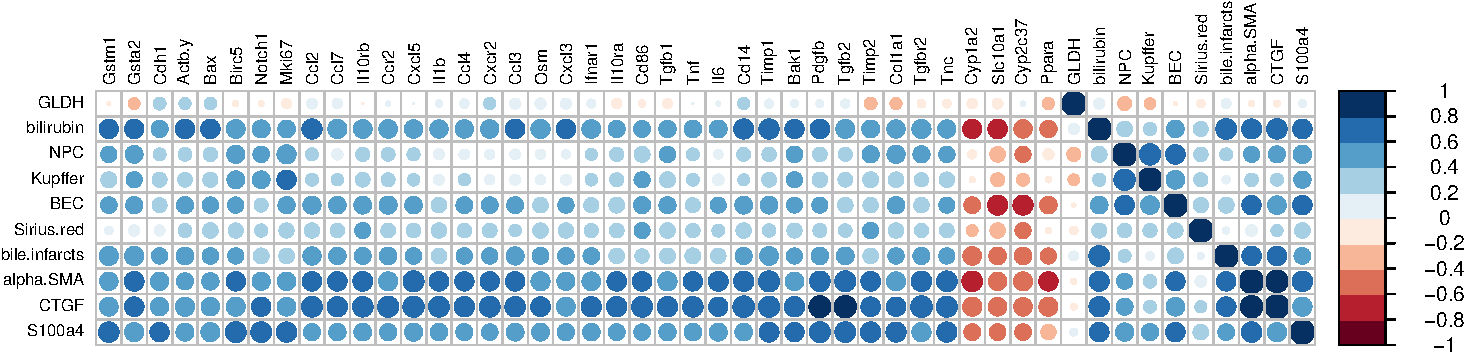
\includegraphics{Figs/histological_correlations_plot-1.pdf}

Figure: Correlations to classical factors. Correlations between
transcripts and classical factors, i.e.~biochemical and
(immuno-)histochemical factors. The genes are filtered based on a cutoff
for the correlation, i.e.~columns in which no correlation coefficient
abs(value) \textgreater{}= cor.cutoff exists are filtered out.

\subsubsection{Top correlations for classical
factors}\label{top-correlations-for-classical-factors}

In the next step the top correlations of every classical factor, i.e.
(immuno-)histochemical (H) and biochemical (B) factors, are calculated,
with the top correlations being sorted by absolute correlation values.

\begin{Shaded}
\begin{Highlighting}[]
\NormalTok{plot_hist_topcors <-}\StringTok{ }\NormalTok{function(}\DataTypeTok{method=}\StringTok{"ys3"}\NormalTok{, }\DataTypeTok{labels=}\OtherTok{TRUE}\NormalTok{, }\DataTypeTok{mfrow=}\KeywordTok{c}\NormalTok{(}\DecValTok{10}\NormalTok{,}\DecValTok{1}\NormalTok{), }
                              \DataTypeTok{only_RNA=}\OtherTok{FALSE}\NormalTok{, }\DataTypeTok{Ntop=}\DecValTok{10}\NormalTok{)\{}
  \NormalTok{hist_facs <-}\StringTok{ }\KeywordTok{rownames}\NormalTok{(histological_correlations)}
  \NormalTok{cor.mat <-}\StringTok{ }\NormalTok{cor.matrices[[method]]}
  
  \CommentTok{# store the results}
  \NormalTok{top.correlations <-}\StringTok{ }\KeywordTok{vector}\NormalTok{(}\StringTok{"list"}\NormalTok{, }\DataTypeTok{length=}\KeywordTok{length}\NormalTok{(hist_facs))}
  \KeywordTok{names}\NormalTok{(top.correlations) <-}\StringTok{ }\NormalTok{hist_facs}
  
  \KeywordTok{par}\NormalTok{(}\DataTypeTok{mfrow=}\NormalTok{mfrow)}
  \NormalTok{hmap_colors <-}\StringTok{ }\KeywordTok{HeatmapColors}\NormalTok{()}
  \NormalTok{for (name in hist_facs)\{}
    \NormalTok{if (only_RNA==}\OtherTok{TRUE}\NormalTok{)\{}
      \CommentTok{# get which which are not classical factors}
      \NormalTok{v <-}\StringTok{ }\NormalTok{cor.mat[!(}\KeywordTok{colnames}\NormalTok{(cor.mat) %in%}\StringTok{ }\NormalTok{hist_facs), name]  }
    \NormalTok{\} else \{}
      \CommentTok{# get all factors (including other non-RNA factors)}
      \NormalTok{v <-}\StringTok{ }\NormalTok{cor.mat[, name]  }
    \NormalTok{\}}
    \CommentTok{# sort by absolute correlation}
    \NormalTok{v.sorted <-}\StringTok{ }\KeywordTok{rev}\NormalTok{(v[}\KeywordTok{order}\NormalTok{(}\KeywordTok{abs}\NormalTok{(v))])}
    \CommentTok{# and get the Ntop values without the self-correlation (idx=1)}
    \NormalTok{mv <-}\StringTok{ }\KeywordTok{t}\NormalTok{(}\KeywordTok{as.matrix}\NormalTok{(v.sorted[}\DecValTok{2}\NormalTok{:(Ntop}\DecValTok{+1}\NormalTok{)]))}
    \KeywordTok{rownames}\NormalTok{(mv) <-}\StringTok{ }\KeywordTok{c}\NormalTok{(name)}
    \CommentTok{# store}
    \NormalTok{top.correlations[[name]] <-}\StringTok{ }\NormalTok{mv}

    \CommentTok{# plot without labels to have identical size of figure}
    \NormalTok{if (labels==}\OtherTok{FALSE}\NormalTok{)\{}
      \KeywordTok{rownames}\NormalTok{(mv) <-}\StringTok{ }\OtherTok{NULL}
      \KeywordTok{colnames}\NormalTok{(mv) <-}\StringTok{ }\OtherTok{NULL}
    \NormalTok{\}}
    \KeywordTok{corrplot}\NormalTok{(mv, }\DataTypeTok{method=}\StringTok{"pie"}\NormalTok{, }\DataTypeTok{type=}\StringTok{"full"}\NormalTok{, }
             \DataTypeTok{tl.cex=}\FloatTok{1.0}\NormalTok{, }\DataTypeTok{tl.col=}\StringTok{"black"}\NormalTok{, }\DataTypeTok{col=}\KeywordTok{hmap_colors}\NormalTok{(}\DecValTok{100}\NormalTok{), }\DataTypeTok{insig=}\StringTok{"p-value"}\NormalTok{, }\DataTypeTok{sig.level=}\NormalTok{-}\DecValTok{1}\NormalTok{,}
             \DataTypeTok{p.mat=}\NormalTok{mv, }\DataTypeTok{cl.pos=}\StringTok{"n"}\NormalTok{)}
  \NormalTok{\}}
  \KeywordTok{par}\NormalTok{(}\DataTypeTok{mfrow=}\KeywordTok{c}\NormalTok{(}\DecValTok{1}\NormalTok{,}\DecValTok{1}\NormalTok{))}
  \KeywordTok{return}\NormalTok{(}\KeywordTok{invisible}\NormalTok{(top.correlations))}
\NormalTok{\}}

\CommentTok{# plot to file}
\CommentTok{# necessary to plot once with and without labels so that all the plots are scaled equally}
\KeywordTok{pdf}\NormalTok{(}\KeywordTok{file.path}\NormalTok{(resultsPath, }\StringTok{"correlation"}\NormalTok{, }\StringTok{"histological_topcors_1.pdf"}\NormalTok{), }
    \DataTypeTok{width=}\DecValTok{10}\NormalTok{, }\DataTypeTok{height=}\DecValTok{10}\NormalTok{, }\DataTypeTok{pointsize=}\DecValTok{12}\NormalTok{)  }
\KeywordTok{plot_hist_topcors}\NormalTok{(}\DataTypeTok{method=}\StringTok{"ys3"}\NormalTok{, }\DataTypeTok{labels=}\OtherTok{TRUE}\NormalTok{)}
\KeywordTok{invisible}\NormalTok{(}\KeywordTok{dev.off}\NormalTok{())}
\KeywordTok{pdf}\NormalTok{(}\KeywordTok{file.path}\NormalTok{(resultsPath, }\StringTok{"correlation"}\NormalTok{, }\StringTok{"histological_topcors_2.pdf"}\NormalTok{), }
    \DataTypeTok{width=}\DecValTok{10}\NormalTok{, }\DataTypeTok{height=}\DecValTok{10}\NormalTok{, }\DataTypeTok{pointsize=}\DecValTok{12}\NormalTok{)  }
\KeywordTok{plot_hist_topcors}\NormalTok{(}\DataTypeTok{method=}\StringTok{"ys3"}\NormalTok{, }\DataTypeTok{labels=}\OtherTok{FALSE}\NormalTok{)}
\KeywordTok{invisible}\NormalTok{(}\KeywordTok{dev.off}\NormalTok{())}
\end{Highlighting}
\end{Shaded}

\begin{Shaded}
\begin{Highlighting}[]
\NormalTok{top.correlations <-}\StringTok{ }\KeywordTok{plot_hist_topcors}\NormalTok{(}\DataTypeTok{method=}\StringTok{"ys3"}\NormalTok{, }\DataTypeTok{labels=}\OtherTok{TRUE}\NormalTok{, }\DataTypeTok{mfrow=}\KeywordTok{c}\NormalTok{(}\DecValTok{5}\NormalTok{,}\DecValTok{2}\NormalTok{))}
\end{Highlighting}
\end{Shaded}

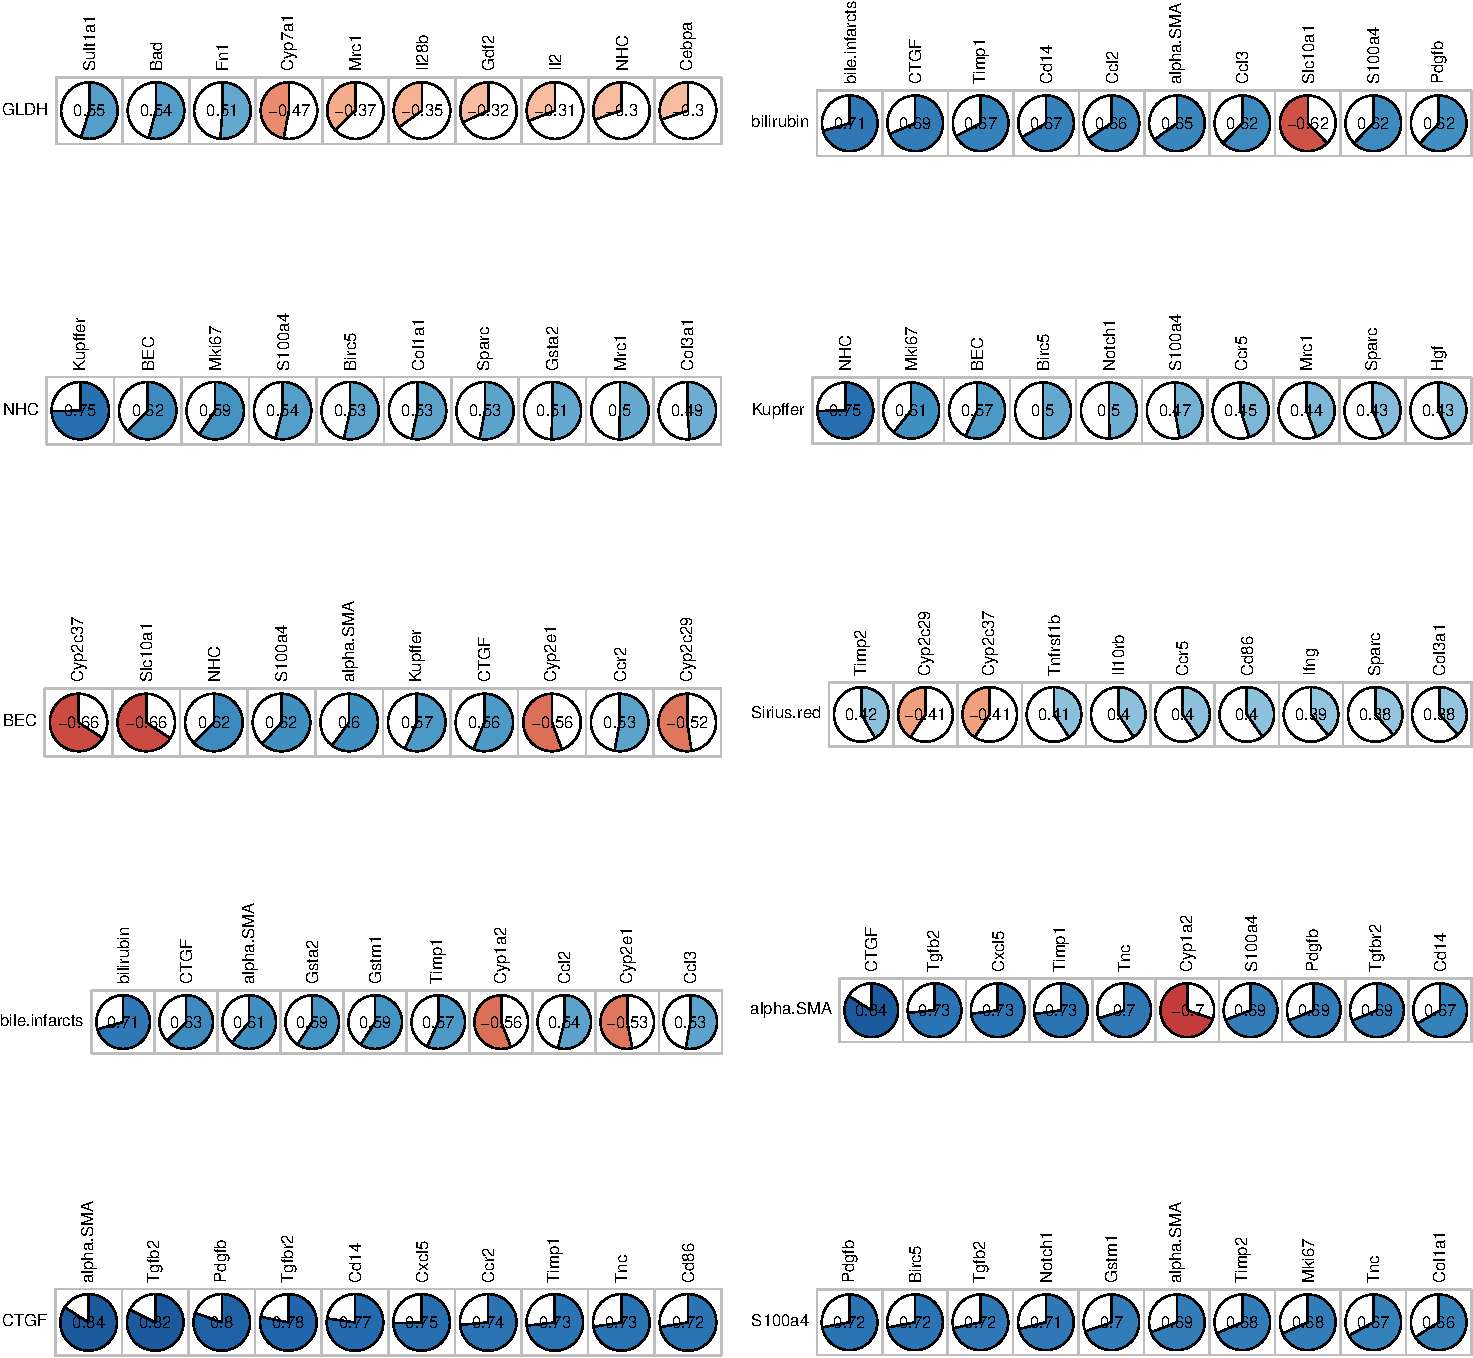
\includegraphics{Figs/plot_hist_topcors_report-1.pdf}

Figure: Top correlations to classical factors.

\small

\begin{Shaded}
\begin{Highlighting}[]
\CommentTok{# print top correlations}
\KeywordTok{options}\NormalTok{(}\DataTypeTok{width=}\DecValTok{200}\NormalTok{)}
\NormalTok{for (mv in top.correlations)\{}
  \KeywordTok{print}\NormalTok{(}\KeywordTok{round}\NormalTok{(mv, }\DataTypeTok{digits=}\DecValTok{2}\NormalTok{)) }
  \KeywordTok{cat}\NormalTok{(}\StringTok{"}\CharTok{\textbackslash{}n}\StringTok{"}\NormalTok{)}
\NormalTok{\}}
\end{Highlighting}
\end{Shaded}

\begin{verbatim}
     Sult1a1  Bad  Fn1 Cyp7a1  Mrc1 Il28b  Gdf2   Il2  NPC Cebpa
GLDH    0.55 0.54 0.51  -0.47 -0.37 -0.35 -0.32 -0.31 -0.3  -0.3

          bile.infarcts CTGF Timp1 Cd14 Ccl2 alpha.SMA Ccl3 Slc10a1 S100a4 Pdgfb
bilirubin          0.71 0.69  0.67 0.67 0.66      0.65 0.62   -0.62   0.62  0.62

    Kupffer  BEC Mki67 S100a4 Birc5 Col1a1 Sparc Gsta2 Mrc1 Col3a1
NPC    0.75 0.62  0.59   0.54  0.53   0.53  0.53  0.51  0.5   0.49

         NPC Mki67  BEC Birc5 Notch1 S100a4 Ccr5 Mrc1 Sparc  Hgf
Kupffer 0.75  0.61 0.57   0.5    0.5   0.47 0.45 0.44  0.43 0.43

    Cyp2c37 Slc10a1  NPC S100a4 alpha.SMA Kupffer CTGF Cyp2e1 Ccr2 Cyp2c29
BEC   -0.66   -0.66 0.62   0.62       0.6    0.57 0.56  -0.56 0.53   -0.52

           Timp2 Cyp2c29 Cyp2c37 Tnfrsf1b Il10rb Ccr5 Cd86 Ifng Sparc Col3a1
Sirius.red  0.42   -0.41   -0.41     0.41    0.4  0.4  0.4 0.39  0.38   0.38

              bilirubin CTGF alpha.SMA Gsta2 Gstm1 Timp1 Cyp1a2 Ccl2 Cyp2e1 Ccl3
bile.infarcts      0.71 0.63      0.61  0.59  0.59  0.57  -0.56 0.54  -0.53 0.53

          CTGF Tgfb2 Cxcl5 Timp1 Tnc Cyp1a2 S100a4 Pdgfb Tgfbr2 Cd14
alpha.SMA 0.84  0.73  0.73  0.73 0.7   -0.7   0.69  0.69   0.69 0.67

     alpha.SMA Tgfb2 Pdgfb Tgfbr2 Cd14 Cxcl5 Ccr2 Timp1  Tnc Cd86
CTGF      0.84  0.82   0.8   0.78 0.77  0.75 0.74  0.73 0.73 0.72

       Pdgfb Birc5 Tgfb2 Notch1 Gstm1 alpha.SMA Timp2 Mki67  Tnc Col1a1
S100a4  0.72  0.72  0.72   0.71   0.7      0.69  0.68  0.68 0.67   0.66
\end{verbatim}

\begin{Shaded}
\begin{Highlighting}[]
\KeywordTok{options}\NormalTok{(}\DataTypeTok{width=}\DecValTok{75}\NormalTok{)}
\KeywordTok{rm}\NormalTok{(mv)}
\end{Highlighting}
\end{Shaded}

\normalsize

\subsection{Mean cluster time course}\label{mean-cluster-time-course}

In the next step, we are interested in the time courses of the found
clusters: What are the typical profiles found in the different clusters
and which factors are in these clusters. For the comparison of
individual factors against each other and against the mean time course
of the cluster the factors were normalized. The normalization was hereby
performed for every factor separately based on
\[f_{k}^{norm}(t_{i,r}) = \frac{f_{k}(t_{i,r})-<f_{k}>}{max(f_{k})-min(f_{k})}\]

\begin{Shaded}
\begin{Highlighting}[]
\KeywordTok{suppressPackageStartupMessages}\NormalTok{(}\KeywordTok{library}\NormalTok{(matrixStats))}
\KeywordTok{dir.create}\NormalTok{(}\KeywordTok{file.path}\NormalTok{(resultsPath, }\StringTok{'cluster'}\NormalTok{), }\DataTypeTok{showWarnings=}\OtherTok{FALSE}\NormalTok{)}

\CommentTok{# normalize single factor}
\NormalTok{normalize_factor <-}\StringTok{ }\NormalTok{function(a, min.a, max.a, mean.a)\{}
  \NormalTok{res <-}\StringTok{ }\NormalTok{(a -}\StringTok{ }\NormalTok{mean.a)/(max.a -}\StringTok{ }\NormalTok{min.a)}
\NormalTok{\}}
\CommentTok{# calculate min, max and mean for all single factors (normalization constants)}
\NormalTok{factor.norm <-}\StringTok{ }\KeywordTok{data.frame}\NormalTok{(}\DataTypeTok{min=}\KeywordTok{apply}\NormalTok{(BDLdata, }\DecValTok{2}\NormalTok{, min, }\DataTypeTok{na.rm=}\OtherTok{TRUE}\NormalTok{), }
                            \DataTypeTok{max=}\KeywordTok{apply}\NormalTok{(BDLdata, }\DecValTok{2}\NormalTok{, max, }\DataTypeTok{na.rm=}\OtherTok{TRUE}\NormalTok{),}
                            \DataTypeTok{mean=}\KeywordTok{apply}\NormalTok{(BDLdata, }\DecValTok{2}\NormalTok{, mean, }\DataTypeTok{na.rm=}\OtherTok{TRUE}\NormalTok{))}
\CommentTok{# function for normalizing subset of BDL data with factor normalization constants.}
\NormalTok{normalize_BDLdata <-}\StringTok{ }\NormalTok{function(data, factor.norm)\{}
  \NormalTok{dnorm <-}\StringTok{ }\NormalTok{data}
  \NormalTok{for (name in }\KeywordTok{colnames}\NormalTok{(data))\{}
    \NormalTok{dnorm[, name] <-}\StringTok{ }\KeywordTok{normalize_factor}\NormalTok{(}\DataTypeTok{a=}\NormalTok{dnorm[, name], }
                                      \DataTypeTok{min.a=}\NormalTok{factor.norm[name, }\StringTok{"min"}\NormalTok{], }
                                      \DataTypeTok{max.a=}\NormalTok{factor.norm[name, }\StringTok{"max"}\NormalTok{],}
                                      \DataTypeTok{mean.a=}\NormalTok{factor.norm[name, }\StringTok{"mean"}\NormalTok{]) }
  \NormalTok{\}}
  \KeywordTok{return}\NormalTok{(dnorm)}
\NormalTok{\}}

\CommentTok{# normalize full data set}
\NormalTok{BDLdata.norm <-}\StringTok{ }\KeywordTok{normalize_BDLdata}\NormalTok{(}\DataTypeTok{data=}\NormalTok{BDLdata, }\DataTypeTok{factor.norm=}\NormalTok{factor.norm)}
\CommentTok{# Calculate the mean of the normalized data set}
\NormalTok{BDLmean.norm <-}\StringTok{ }\KeywordTok{bdl_mean_data}\NormalTok{(BDLdata.norm, BDLsamples)}
\end{Highlighting}
\end{Shaded}

With the normalized factor data the mean time course of the 6 clusters
are calculated, i.e.~the time course resulting from averaging over all
members of the individual clusters. Additionally, the mean time course
averaged over the repeats for all factors are plotted.

\begin{Shaded}
\begin{Highlighting}[]
\CommentTok{# Plot mean cluster with SD range and the individual representatives in the cluster.}
\NormalTok{plot_clusters_mean <-}\StringTok{ }\NormalTok{function(method)\{  }
  \CommentTok{# clusters for correlation method}
  \NormalTok{hc.res <-}\StringTok{ }\NormalTok{hclust.res[[method]]}
  \NormalTok{groups.hc.order <-}\StringTok{ }\NormalTok{hc.res$groups.hc.order}

  \CommentTok{# par(mfrow=c(ceiling(sqrt(Ngroups)),ceiling(sqrt(Ngroups))))}
  \KeywordTok{par}\NormalTok{(}\DataTypeTok{mfrow=}\KeywordTok{c}\NormalTok{(}\DecValTok{2}\NormalTok{,}\DecValTok{3}\NormalTok{))}
  \NormalTok{steps <-}\StringTok{ }\DecValTok{1}\NormalTok{:Nt  }\CommentTok{# time points}
  \NormalTok{for (k in }\DecValTok{1}\NormalTok{:Ngroups)\{}
    \CommentTok{# get representatives of cluster}
    \NormalTok{g <-}\StringTok{ }\NormalTok{groups.hc.order[groups.hc.order==k]}
    \NormalTok{dgroup <-}\StringTok{ }\NormalTok{BDLmean.norm[}\KeywordTok{names}\NormalTok{(g)]  }\CommentTok{# normalized mean data for cluster members}
  
    \CommentTok{# mean and sd for timepoints (i.e. over all factors in the cluster) }
    \NormalTok{g.mean <-}\StringTok{ }\KeywordTok{rowMeans}\NormalTok{(}\KeywordTok{as.matrix}\NormalTok{(dgroup), }\DataTypeTok{na.rm=}\OtherTok{TRUE}\NormalTok{)}
    \NormalTok{g.sd <-}\StringTok{ }\KeywordTok{rowSds}\NormalTok{(}\KeywordTok{as.matrix}\NormalTok{(dgroup), }\DataTypeTok{na.rm=}\OtherTok{TRUE}\NormalTok{) }
    
    \CommentTok{# plot sd range}
    \KeywordTok{plot}\NormalTok{(}\KeywordTok{factor}\NormalTok{(}\KeywordTok{levels}\NormalTok{(BDLsamples$time_fac), }\DataTypeTok{levels=}\KeywordTok{levels}\NormalTok{(BDLsamples$time_fac)), }
         \KeywordTok{rep}\NormalTok{(-}\DecValTok{2}\NormalTok{, }\DecValTok{8}\NormalTok{), }\DataTypeTok{type=}\StringTok{"n"}\NormalTok{, }\DataTypeTok{xlab=}\StringTok{""}\NormalTok{, }\DataTypeTok{ylab=}\StringTok{""}\NormalTok{,}
         \DataTypeTok{xlim=}\KeywordTok{c}\NormalTok{(}\DecValTok{1}\NormalTok{, Nt), }\DataTypeTok{ylim=}\FloatTok{1.1}\NormalTok{*}\KeywordTok{c}\NormalTok{( }\KeywordTok{min}\NormalTok{(}\KeywordTok{min}\NormalTok{(dgroup, }\DataTypeTok{na.rm=}\OtherTok{TRUE}\NormalTok{), }\DataTypeTok{na.rm=}\OtherTok{TRUE}\NormalTok{), }
                                    \KeywordTok{max}\NormalTok{(}\KeywordTok{max}\NormalTok{(dgroup, }\DataTypeTok{na.rm=}\OtherTok{TRUE}\NormalTok{), }\DataTypeTok{na.rm=}\OtherTok{TRUE}\NormalTok{) ),}
         \DataTypeTok{main=}\KeywordTok{sprintf}\NormalTok{(}\StringTok{"%s : Cluster %s (N=%s)"}\NormalTok{, method, k, }\KeywordTok{ncol}\NormalTok{(dgroup)))}
    \KeywordTok{polygon}\NormalTok{(}\KeywordTok{c}\NormalTok{(steps, }\KeywordTok{rev}\NormalTok{(steps)), }\KeywordTok{c}\NormalTok{(g.mean+g.sd, }\KeywordTok{rev}\NormalTok{(g.mean-g.sd)),}
            \DataTypeTok{col =} \KeywordTok{rgb}\NormalTok{(}\DecValTok{0}\NormalTok{,}\DecValTok{0}\NormalTok{,}\DecValTok{1}\NormalTok{,}\FloatTok{0.2}\NormalTok{), }\DataTypeTok{border =} \OtherTok{NA}\NormalTok{)}
    
    \CommentTok{# individual data}
    \NormalTok{for (name in }\KeywordTok{names}\NormalTok{(g))\{}
      \KeywordTok{points}\NormalTok{(steps, dgroup[, name], }\DataTypeTok{pch=}\DecValTok{16}\NormalTok{, }\DataTypeTok{col=}\StringTok{"black"}\NormalTok{)}
      \KeywordTok{lines}\NormalTok{(steps, dgroup[, name], }\DataTypeTok{col=}\KeywordTok{rgb}\NormalTok{(}\FloatTok{0.5}\NormalTok{,}\FloatTok{0.5}\NormalTok{,}\FloatTok{0.5}\NormalTok{,}\FloatTok{1.0}\NormalTok{), }\DataTypeTok{lwd=}\DecValTok{1}\NormalTok{)}
    \NormalTok{\}}
    \CommentTok{# mean over factors in cluster}
    \KeywordTok{lines}\NormalTok{(steps, g.mean, }\DataTypeTok{col=}\StringTok{"blue"}\NormalTok{, }\DataTypeTok{lwd=}\DecValTok{2}\NormalTok{)}
  \NormalTok{\}}
  \KeywordTok{par}\NormalTok{(}\DataTypeTok{mfrow=}\KeywordTok{c}\NormalTok{(}\DecValTok{1}\NormalTok{,}\DecValTok{1}\NormalTok{))}
\NormalTok{\}}

\CommentTok{# plot mean clusters to file}
\NormalTok{for (method in correlation_methods)\{}
  \KeywordTok{pdf}\NormalTok{(}\KeywordTok{file.path}\NormalTok{(resultsPath, }\StringTok{'cluster'}\NormalTok{, }\KeywordTok{sprintf}\NormalTok{(}\StringTok{"%s_cluster_mean.pdf"}\NormalTok{, method)), }
        \DataTypeTok{width=}\DecValTok{10}\NormalTok{, }\DataTypeTok{height=}\FloatTok{7.5}\NormalTok{, }\DataTypeTok{pointsize=}\DecValTok{12}\NormalTok{)}
  \KeywordTok{plot_clusters_mean}\NormalTok{(}\DataTypeTok{method=}\NormalTok{method) }
  \KeywordTok{invisible}\NormalTok{(}\KeywordTok{dev.off}\NormalTok{())}
\NormalTok{\}}
\end{Highlighting}
\end{Shaded}

\begin{Shaded}
\begin{Highlighting}[]
\KeywordTok{plot_clusters_mean}\NormalTok{(}\DataTypeTok{method=}\StringTok{"ys3"}\NormalTok{)}
\end{Highlighting}
\end{Shaded}

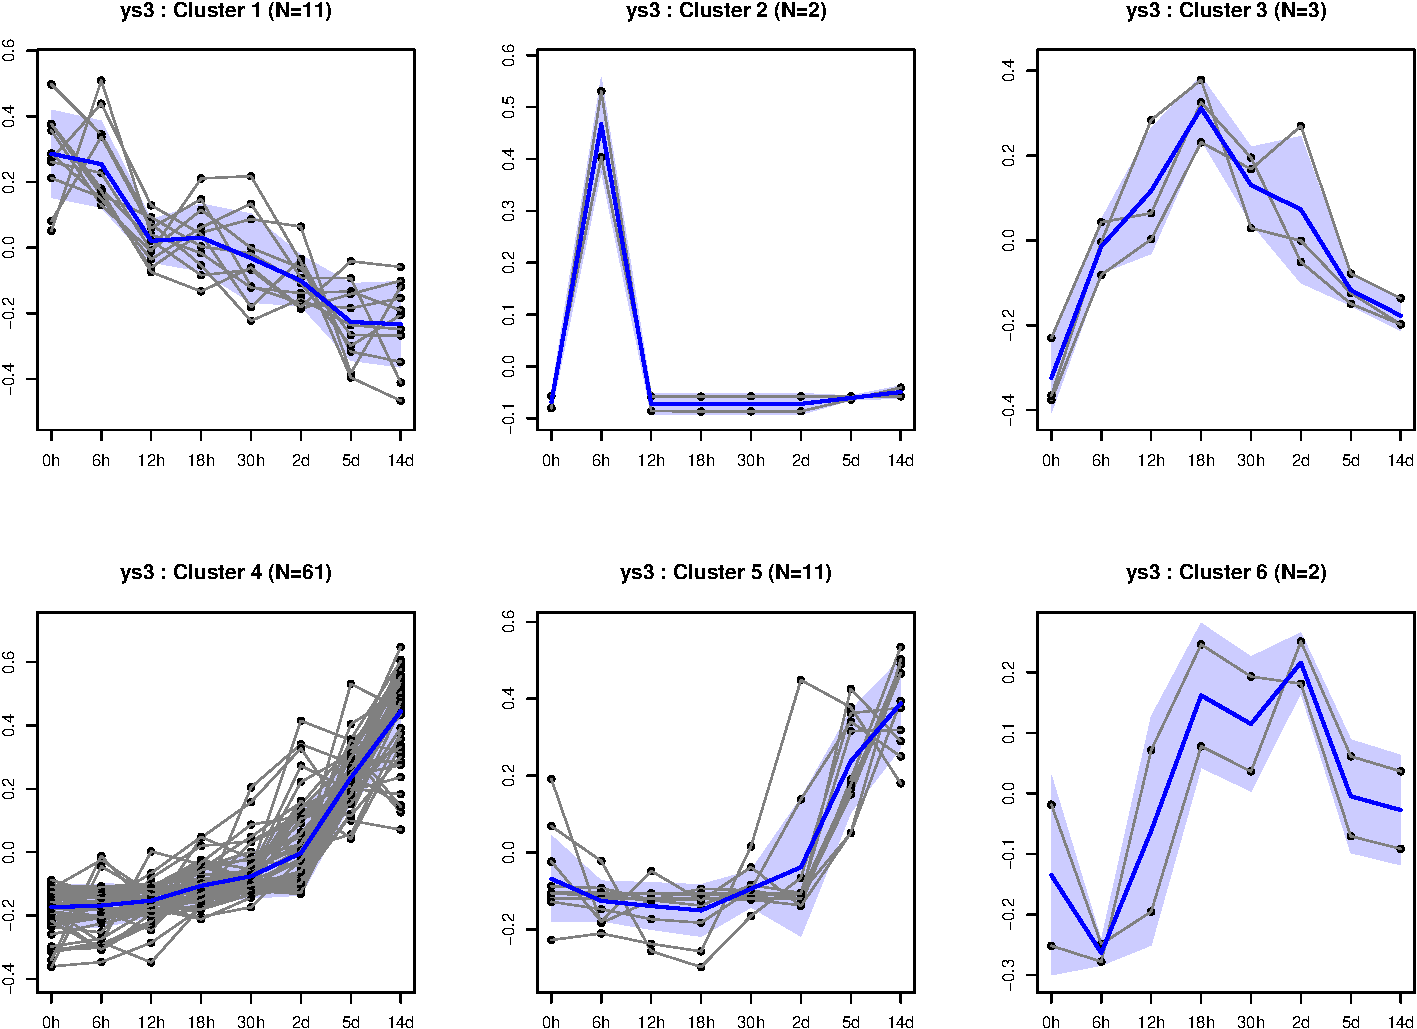
\includegraphics{Figs/plot_clusters_mean_report-1.pdf}

Figure: Mean cluster time courses. Mean time course of clusters in blue,
with individual mean factors in cluster in grey. Standard deviation of
members in cluster is added as gray shade.

In addition the plots of the individual factors in the clusters are
generated. Despite being clustered together still quit large variance
exists between the different factors in the clusters.

\begin{Shaded}
\begin{Highlighting}[]
\CommentTok{# Plot individual time courses in cluster}
\NormalTok{plot_clusters_items <-}\StringTok{ }\NormalTok{function(method, }\DataTypeTok{toFile=}\OtherTok{FALSE}\NormalTok{)\{}
  \CommentTok{# get the cluster assignment for the given method}
  \NormalTok{hc.res <-}\StringTok{ }\NormalTok{hclust.res[[method]]}
  \NormalTok{groups.hc.order <-}\StringTok{ }\NormalTok{hc.res$groups.hc.order}
  
  \NormalTok{for (k in }\DecValTok{1}\NormalTok{:Ngroups)\{}
    \NormalTok{if (toFile==}\OtherTok{TRUE}\NormalTok{)\{}
      \KeywordTok{pdf}\NormalTok{(}\KeywordTok{file.path}\NormalTok{(resultsPath, }\StringTok{"cluster"}\NormalTok{, }\KeywordTok{sprintf}\NormalTok{(}\StringTok{"%s_cluster_%s.pdf"}\NormalTok{, method, k)), }
          \DataTypeTok{width=}\DecValTok{10}\NormalTok{, }\DataTypeTok{height=}\DecValTok{10}\NormalTok{, }\DataTypeTok{pointsize=}\DecValTok{8}\NormalTok{)}
    \NormalTok{\}}
    \NormalTok{g <-}\StringTok{ }\NormalTok{groups.hc.order[groups.hc.order==k]}
    \NormalTok{N <-}\StringTok{ }\KeywordTok{ceiling}\NormalTok{(}\KeywordTok{sqrt}\NormalTok{(}\KeywordTok{length}\NormalTok{(g)))}
    \KeywordTok{par}\NormalTok{(}\DataTypeTok{mfrow=}\KeywordTok{c}\NormalTok{(N,N))}
    \NormalTok{for (name in }\KeywordTok{names}\NormalTok{(g))\{}
      \KeywordTok{plot_single}\NormalTok{(}\DataTypeTok{name_A=}\NormalTok{name) }
    \NormalTok{\}}
    \KeywordTok{par}\NormalTok{(}\DataTypeTok{mfrow=}\KeywordTok{c}\NormalTok{(}\DecValTok{1}\NormalTok{,}\DecValTok{1}\NormalTok{))  }
    \NormalTok{if (toFile==}\OtherTok{TRUE}\NormalTok{)\{}
      \KeywordTok{invisible}\NormalTok{(}\KeywordTok{dev.off}\NormalTok{())}
    \NormalTok{\}}
  \NormalTok{\}  }
\NormalTok{\}}

\CommentTok{# plot individual factors in clusters on disk}
\NormalTok{for (method in correlation_methods)\{}
  \KeywordTok{plot_clusters_items}\NormalTok{(}\DataTypeTok{method=}\NormalTok{method, }\DataTypeTok{toFile=}\OtherTok{TRUE}\NormalTok{)  }
\NormalTok{\}}
\KeywordTok{rm}\NormalTok{(method)}
\end{Highlighting}
\end{Shaded}

\subsection{Top cluster
representatives}\label{top-cluster-representatives}

In this step, the top cluster representatives are calculated for all
clusters. The higher the correlation between the factor and the cluster
mean, the higher the respective factor is scored. The used correlation
measure is \texttt{YS3}. The result are the correlation matrices for the
individual clusters.

\begin{Shaded}
\begin{Highlighting}[]
\NormalTok{hmap_colors <-}\StringTok{ }\KeywordTok{HeatmapColors}\NormalTok{()}

\CommentTok{# correlation between the cluster mean and cluster members}
\NormalTok{calculate_cluster_correlations <-}\StringTok{ }\NormalTok{function(}\DataTypeTok{method=}\StringTok{"ys3"}\NormalTok{)\{}
  \NormalTok{if (!}\KeywordTok{identical}\NormalTok{(method, }\StringTok{"ys3"}\NormalTok{))\{}
    \KeywordTok{stop}\NormalTok{(}\StringTok{"Only ys3 top correlation is currently supported"}\NormalTok{)}
  \NormalTok{\}}
  \CommentTok{# get the clusters}
  \NormalTok{hc.res <-}\StringTok{ }\NormalTok{hclust.res[[method]]}
  \NormalTok{groups.hc.order <-}\StringTok{ }\NormalTok{hc.res$groups.hc.order}
  \CommentTok{# mean cluster time course as additional factor}
  \NormalTok{name_cluster <-}\StringTok{ }\KeywordTok{sprintf}\NormalTok{(}\StringTok{"cluster.mean"}\NormalTok{)}
  
  \CommentTok{# calculate top correlations for every cluster}
  \NormalTok{cluster.cor <-}\StringTok{ }\KeywordTok{vector}\NormalTok{(}\StringTok{"list"}\NormalTok{, }\DataTypeTok{length=}\NormalTok{Ngroups)}
  \NormalTok{for (k in }\DecValTok{1}\NormalTok{:Ngroups)\{}
      \CommentTok{# get members of cluster}
      \NormalTok{g <-}\StringTok{ }\NormalTok{groups.hc.order[groups.hc.order==k]}
      \CommentTok{# get normalized data for members of cluster}
      \NormalTok{dgroup <-}\StringTok{ }\NormalTok{BDLdata.norm[}\KeywordTok{names}\NormalTok{(g)]}
      \CommentTok{# cluster mean and add as factor (mean of all factors in cluster }
      \CommentTok{# for given time point and sample)}
      \NormalTok{g.mean <-}\StringTok{ }\KeywordTok{rowMeans}\NormalTok{(}\KeywordTok{as.matrix}\NormalTok{(dgroup), }\DataTypeTok{na.rm=}\OtherTok{TRUE}\NormalTok{)}
      \NormalTok{dgroup[[name_cluster]] <-}\StringTok{ }\NormalTok{g.mean}
      \CommentTok{# mean averaged over repeats (for A** and M*)}
      \NormalTok{dgroup.mean <-}\StringTok{ }\KeywordTok{bdl_mean_data}\NormalTok{(dgroup, BDLsamples)}
      \CommentTok{# ys3 correlation for created data.frame with mean cluster factor}
      \NormalTok{ysr.res <-}\StringTok{ }\KeywordTok{ysr.matrices}\NormalTok{(dgroup.mean, BDLmean.time, }\DataTypeTok{use=}\StringTok{"pairwise.complete.obs"}\NormalTok{)}
      \CommentTok{# Spearman correlation on individual data points}
      \NormalTok{cor.S_star <-}\StringTok{ }\NormalTok{( }\KeywordTok{cor}\NormalTok{(dgroup, }\DataTypeTok{method=}\StringTok{"spearman"}\NormalTok{, }\DataTypeTok{use=}\StringTok{"pairwise.complete.obs"}\NormalTok{) +}\StringTok{ }\DecValTok{1} \NormalTok{)/}\DecValTok{2}
      \CommentTok{# YS3 in [-1,1]}
      \NormalTok{ys3 <-}\StringTok{ }\DecValTok{2}\NormalTok{*( (w$w1*cor.S_star +}\StringTok{ }\NormalTok{w$w2*ysr.res$A_star2 +}\StringTok{ }\NormalTok{w$w3*ysr.res$M_star) -}\StringTok{ }\FloatTok{0.5}\NormalTok{)}
      \CommentTok{# store correlation matrix}
      \NormalTok{cluster.cor[[k]] <-}\StringTok{ }\NormalTok{ys3}
  \NormalTok{\}}
  \KeywordTok{return}\NormalTok{(cluster.cor)}
\NormalTok{\}}
\NormalTok{cluster.cor <-}\StringTok{ }\KeywordTok{calculate_cluster_correlations}\NormalTok{(}\DataTypeTok{method=}\StringTok{"ys3"}\NormalTok{)}
\end{Highlighting}
\end{Shaded}

\begin{Shaded}
\begin{Highlighting}[]
\CommentTok{# plot correlations for individual clusters}
\NormalTok{for (k in }\DecValTok{1}\NormalTok{:Ngroups)\{}
  \NormalTok{cluster.cor.mat <-}\StringTok{ }\NormalTok{cluster.cor[[k]]}
  \NormalTok{if (}\KeywordTok{ncol}\NormalTok{(cluster.cor.mat)<}\DecValTok{20}\NormalTok{)\{}
    \KeywordTok{corrplot}\NormalTok{(cluster.cor.mat, }\DataTypeTok{method=}\StringTok{"pie"}\NormalTok{, }\DataTypeTok{type=}\StringTok{"full"}\NormalTok{, }
           \DataTypeTok{main=}\KeywordTok{sprintf}\NormalTok{(}\StringTok{"Cluster %s"}\NormalTok{, k),}
             \DataTypeTok{tl.cex=}\FloatTok{0.8}\NormalTok{, }\DataTypeTok{tl.col=}\StringTok{"black"}\NormalTok{, }\DataTypeTok{col=}\KeywordTok{hmap_colors}\NormalTok{(}\DecValTok{100}\NormalTok{), }
             \DataTypeTok{insig=}\StringTok{"p-value"}\NormalTok{, }\DataTypeTok{sig.level=}\NormalTok{-}\DecValTok{1}\NormalTok{, }\DataTypeTok{p.mat=}\NormalTok{cluster.cor.mat,}
             \DataTypeTok{cl.pos=}\StringTok{"n"}\NormalTok{)}
  \NormalTok{\} else \{}
    \KeywordTok{corrplot}\NormalTok{(cluster.cor.mat, }\DataTypeTok{method=}\StringTok{"circle"}\NormalTok{, }\DataTypeTok{type=}\StringTok{"full"}\NormalTok{, }
           \DataTypeTok{main=}\KeywordTok{sprintf}\NormalTok{(}\StringTok{"Cluster %s"}\NormalTok{, k),}
             \DataTypeTok{tl.cex=}\FloatTok{0.8}\NormalTok{, }\DataTypeTok{tl.col=}\StringTok{"black"}\NormalTok{, }\DataTypeTok{col=}\KeywordTok{hmap_colors}\NormalTok{(}\DecValTok{100}\NormalTok{), }
             \DataTypeTok{cl.pos=}\StringTok{"n"}\NormalTok{)}
  \NormalTok{\}}
\NormalTok{\}}
\KeywordTok{rm}\NormalTok{(k, cluster.cor.mat)}
\end{Highlighting}
\end{Shaded}

From the cluster correlation matrices the top correlations between
cluster mean and the members of the respective cluster can be extracted.

\begin{Shaded}
\begin{Highlighting}[]
\NormalTok{plot_top_cluster_representatives <-}\StringTok{ }\NormalTok{function(}\DataTypeTok{method=}\StringTok{"ys3"}\NormalTok{, }\DataTypeTok{Ntop=}\DecValTok{11}\NormalTok{, }\DataTypeTok{labels=}\OtherTok{TRUE}\NormalTok{)\{}
  \KeywordTok{par}\NormalTok{(}\DataTypeTok{mfrow=}\KeywordTok{c}\NormalTok{(Ngroups,}\DecValTok{1}\NormalTok{))}
  \NormalTok{name_cluster <-}\StringTok{ }\KeywordTok{sprintf}\NormalTok{(}\StringTok{"cluster.mean"}\NormalTok{)}
  \NormalTok{for (k in }\DecValTok{1}\NormalTok{:Ngroups)\{}
      \CommentTok{# YS3 in [-1,1]}
      \NormalTok{ys3 <-}\StringTok{ }\NormalTok{cluster.cor[[k]]}
  
      \CommentTok{# correlation for the cluster mean}
      \NormalTok{v <-}\StringTok{ }\NormalTok{ys3[, }\KeywordTok{which}\NormalTok{(}\KeywordTok{colnames}\NormalTok{(ys3)==name_cluster)]}
      \CommentTok{# sort by absolute correlation}
      \NormalTok{v.sorted <-}\StringTok{ }\KeywordTok{rev}\NormalTok{(v[}\KeywordTok{order}\NormalTok{(}\KeywordTok{abs}\NormalTok{(v))])}

      \CommentTok{# reduce to Ntop candidates and fill short clusters with zeros tto Ntop}
      \NormalTok{if (}\KeywordTok{length}\NormalTok{(v.sorted)>=(Ntop}\DecValTok{+1}\NormalTok{))\{}
        \NormalTok{v.sorted <-}\StringTok{ }\NormalTok{v.sorted[}\DecValTok{2}\NormalTok{:(Ntop}\DecValTok{+1}\NormalTok{)]}
      \NormalTok{\} else \{}
        \NormalTok{v.sorted <-}\StringTok{ }\KeywordTok{c}\NormalTok{(v.sorted[}\DecValTok{2}\NormalTok{:}\KeywordTok{length}\NormalTok{(v.sorted)], }\KeywordTok{rep}\NormalTok{(}\DecValTok{0}\NormalTok{,Ntop-}\KeywordTok{length}\NormalTok{(v.sorted)+}\DecValTok{1}\NormalTok{))}
      \NormalTok{\}}
      \CommentTok{# prepare data for corrplot}
      \NormalTok{mv <-}\StringTok{ }\KeywordTok{t}\NormalTok{(}\KeywordTok{as.matrix}\NormalTok{(v.sorted))}
      \KeywordTok{rownames}\NormalTok{(mv) <-}\StringTok{ }\KeywordTok{c}\NormalTok{(}\KeywordTok{paste}\NormalTok{(name_cluster, k))}
      \NormalTok{if (labels ==}\StringTok{ }\OtherTok{FALSE}\NormalTok{)\{}
        \KeywordTok{colnames}\NormalTok{(mv) <-}\StringTok{ }\OtherTok{NULL}
      \NormalTok{\}}
      \KeywordTok{corrplot}\NormalTok{(mv, }\DataTypeTok{method=}\StringTok{"pie"}\NormalTok{, }\DataTypeTok{type=}\StringTok{"full"}\NormalTok{, }
             \DataTypeTok{tl.cex=}\FloatTok{1.0}\NormalTok{, }\DataTypeTok{tl.col=}\StringTok{"black"}\NormalTok{, }\DataTypeTok{col=}\KeywordTok{hmap_colors}\NormalTok{(}\DecValTok{100}\NormalTok{), }
             \DataTypeTok{insig=}\StringTok{"p-value"}\NormalTok{, }\DataTypeTok{sig.level=}\NormalTok{-}\DecValTok{1}\NormalTok{, }\DataTypeTok{p.mat=}\NormalTok{mv,}
             \DataTypeTok{cl.pos=}\StringTok{"n"}\NormalTok{)}
  \NormalTok{\}}
  \KeywordTok{par}\NormalTok{(}\DataTypeTok{mfrow=}\KeywordTok{c}\NormalTok{(}\DecValTok{1}\NormalTok{,}\DecValTok{1}\NormalTok{))}
\NormalTok{\}}

\CommentTok{# plot to file (with and without names)}
\KeywordTok{pdf}\NormalTok{(}\KeywordTok{file.path}\NormalTok{(resultsPath, }\StringTok{"cluster"}\NormalTok{, }\StringTok{"cluster_top_representatives_01.pdf"}\NormalTok{), }
    \DataTypeTok{width=}\DecValTok{5}\NormalTok{, }\DataTypeTok{height=}\DecValTok{5}\NormalTok{, }\DataTypeTok{pointsize=}\DecValTok{12}\NormalTok{)}
\KeywordTok{plot_top_cluster_representatives}\NormalTok{(}\DataTypeTok{labels=}\OtherTok{FALSE}\NormalTok{)}
\KeywordTok{invisible}\NormalTok{(}\KeywordTok{dev.off}\NormalTok{())}
\KeywordTok{pdf}\NormalTok{(}\KeywordTok{file.path}\NormalTok{(resultsPath, }\StringTok{"cluster"}\NormalTok{, }\StringTok{"cluster_top_representatives_02.pdf"}\NormalTok{), }
    \DataTypeTok{width=}\DecValTok{10}\NormalTok{, }\DataTypeTok{height=}\DecValTok{10}\NormalTok{, }\DataTypeTok{pointsize=}\DecValTok{12}\NormalTok{)}
\KeywordTok{plot_top_cluster_representatives}\NormalTok{(}\DataTypeTok{labels=}\OtherTok{TRUE}\NormalTok{)}
\KeywordTok{invisible}\NormalTok{(}\KeywordTok{dev.off}\NormalTok{())}
\end{Highlighting}
\end{Shaded}

\begin{Shaded}
\begin{Highlighting}[]
\KeywordTok{plot_top_cluster_representatives}\NormalTok{(}\DataTypeTok{labels=}\OtherTok{TRUE}\NormalTok{)}
\end{Highlighting}
\end{Shaded}

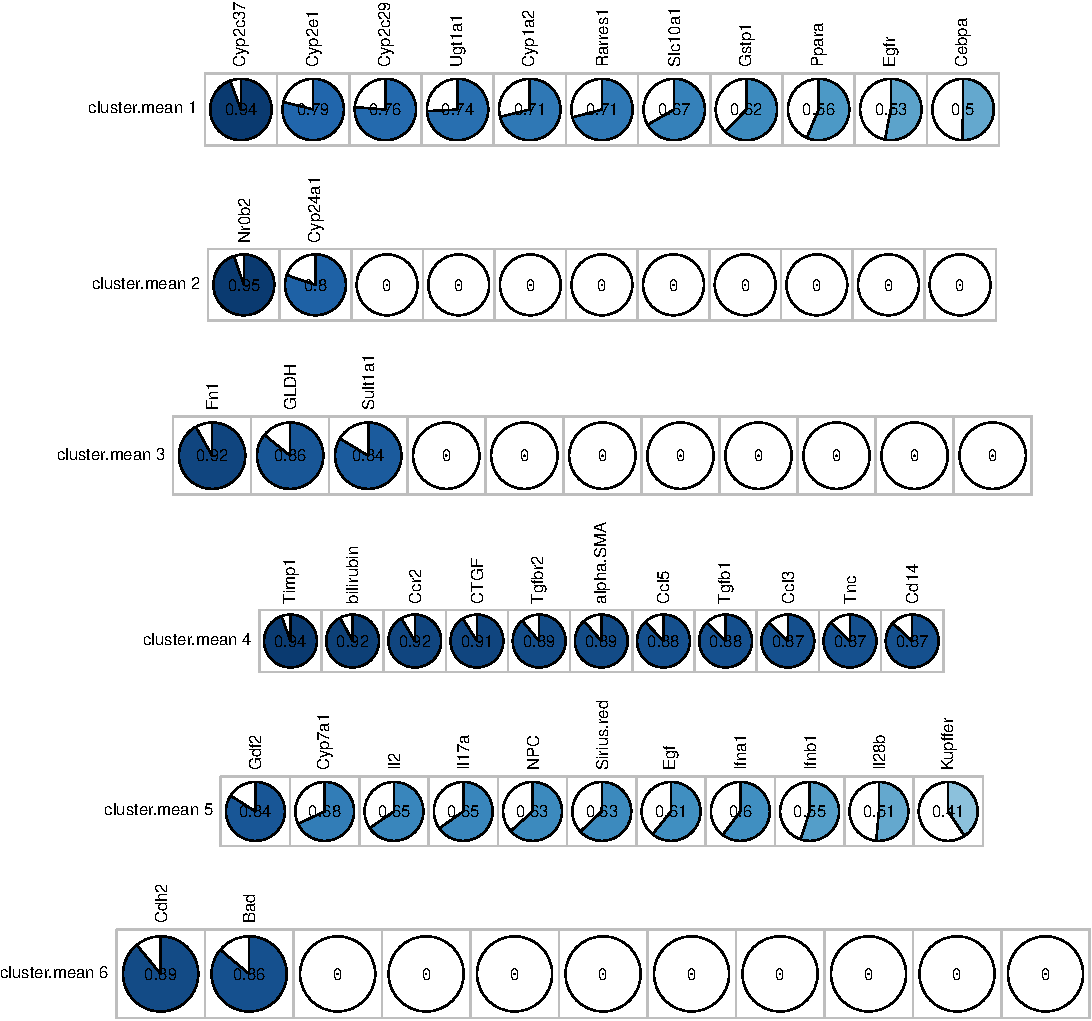
\includegraphics{Figs/plot_clusters_top_correlations-1.pdf}

Figure: Top cluster correlations. Top correlations between the
respective cluster mean and the members in the cluster sorted by
absolute correlation.

\subsection{YS3 cluster summary}\label{ys3-cluster-summary}

Overview over the members of the 6 clusters with respective YS3
correlation to the cluster mean and ANOVA result.

\begin{Shaded}
\begin{Highlighting}[]
\CommentTok{# print representatives of cluster}
\NormalTok{list_cluster_information <-}\StringTok{ }\NormalTok{function(}\DataTypeTok{method=}\StringTok{"ys3"}\NormalTok{)\{}
  \NormalTok{if(!}\KeywordTok{identical}\NormalTok{(method, }\StringTok{"ys3"}\NormalTok{))\{}
    \KeywordTok{stop}\NormalTok{(}\StringTok{"Cluster correlation only calculated for ys3"}\NormalTok{)}
  \NormalTok{\}}
  \NormalTok{groups <-}\StringTok{ }\NormalTok{hclust.res[[method]]$groups}
  \KeywordTok{cat}\NormalTok{(}\KeywordTok{sprintf}\NormalTok{(}\StringTok{"------------------------------------------}\CharTok{\textbackslash{}n}\StringTok{"}\NormalTok{))}
  \KeywordTok{cat}\NormalTok{(}\KeywordTok{sprintf}\NormalTok{(}\StringTok{"Correlation method: *** %s ***}\CharTok{\textbackslash{}n}\StringTok{"}\NormalTok{, method))}
  \KeywordTok{cat}\NormalTok{(}\KeywordTok{sprintf}\NormalTok{(}\StringTok{"------------------------------------------}\CharTok{\textbackslash{}n}\StringTok{"}\NormalTok{))}
  \NormalTok{for (k in }\DecValTok{1}\NormalTok{:Ngroups)\{}
    \NormalTok{cluster.cor.mat <-}\StringTok{ }\NormalTok{cluster.cor[[k]]}
    \CommentTok{# create data.frame with ANOVA & cluster correlation}
    \NormalTok{g <-}\StringTok{ }\NormalTok{groups[groups==k]}
    \KeywordTok{cat}\NormalTok{(}\KeywordTok{sprintf}\NormalTok{(}\StringTok{"Cluster %s (N=%s)}\CharTok{\textbackslash{}n}\StringTok{"}\NormalTok{, k, }\KeywordTok{length}\NormalTok{(g)))}
    \NormalTok{Ng <-}\StringTok{ }\KeywordTok{length}\NormalTok{(}\KeywordTok{names}\NormalTok{(g))}
    \NormalTok{rows <-}\StringTok{ }\KeywordTok{vector}\NormalTok{(}\StringTok{"list"}\NormalTok{, }\DataTypeTok{length=}\NormalTok{Ng)}
    \NormalTok{for (kn in }\DecValTok{1}\NormalTok{:Ng)\{}
      \NormalTok{name <-}\StringTok{ }\KeywordTok{names}\NormalTok{(g)[kn]}
      \NormalTok{row <-}\StringTok{ }\NormalTok{df.anova[}\KeywordTok{which}\NormalTok{(df.anova$factor==name),]}
      \NormalTok{row$cluster.cor <-}\StringTok{ }\NormalTok{cluster.cor.mat[name, }\StringTok{"cluster.mean"}\NormalTok{]}
      \NormalTok{rows[[kn]] <-}\StringTok{ }\NormalTok{row}
    \NormalTok{\}}
    \NormalTok{df <-}\StringTok{ }\KeywordTok{do.call}\NormalTok{(}\StringTok{"rbind"}\NormalTok{, rows)}
    \NormalTok{df <-}\StringTok{ }\NormalTok{df[}\KeywordTok{order}\NormalTok{(-df$cluster.cor), ]}

    \CommentTok{# cleanup the data.frame}
    \KeywordTok{rownames}\NormalTok{(df) <-}\StringTok{ }\NormalTok{df$factors}
    \NormalTok{df <-}\StringTok{ }\NormalTok{df[, }\KeywordTok{c}\NormalTok{(}\StringTok{"p.holm"}\NormalTok{, }\StringTok{"sig.holm"}\NormalTok{, }\StringTok{"ftype"}\NormalTok{, }\StringTok{"fshort"}\NormalTok{, }\StringTok{"cluster.cor"}\NormalTok{)]}
    \NormalTok{df$cluster.cor <-}\StringTok{ }\KeywordTok{round}\NormalTok{(df$cluster.cor, }\DataTypeTok{digits=}\DecValTok{2}\NormalTok{)}
    \NormalTok{df$p.holm <-}\StringTok{ }\KeywordTok{sprintf}\NormalTok{(}\StringTok{"%1.2E"}\NormalTok{, df$p.holm)}
    \KeywordTok{print}\NormalTok{(df)}
    
    \KeywordTok{cat}\NormalTok{(}\StringTok{"}\CharTok{\textbackslash{}n}\StringTok{"}\NormalTok{)}
    \CommentTok{# create list for figure legend}
    \CommentTok{# print(paste(sprintf("%s (%s)", rownames(df), df$cluster.cor),}
    \CommentTok{#            sep=", ", collapse =", " ))}
  \NormalTok{\}  }
\NormalTok{\}}
\end{Highlighting}
\end{Shaded}

\small

\begin{Shaded}
\begin{Highlighting}[]
\CommentTok{# List information in cluster}
\KeywordTok{list_cluster_information}\NormalTok{(}\DataTypeTok{method=}\StringTok{"ys3"}\NormalTok{)}
\end{Highlighting}
\end{Shaded}

\begin{verbatim}
------------------------------------------
Correlation method: *** ys3 ***
------------------------------------------
Cluster 1 (N=11)
          p.holm sig.holm        ftype fshort cluster.cor
Cyp2c37 1.09E-05      ***      GE_ADME               0.94
Cyp2e1  1.50E-06      ***  GE_Fibrosis               0.79
Cyp2c29 2.93E-06      ***      GE_ADME               0.76
Ugt1a1  2.75E-03       **      GE_ADME               0.74
Cyp1a2  2.93E-14      ***      GE_ADME               0.71
Rarres1 3.57E-02        *  GE_Fibrosis               0.71
Slc10a1 5.26E-05      ***      GE_ADME               0.67
Gstp1   1.38E-04      ***      GE_ADME               0.62
Ppara   1.63E-04      ***      GE_ADME               0.56
Egfr    1.59E-03       ** GE_Cytokines               0.53
Cebpa   4.93E-04      ***      GE_ADME               0.50

Cluster 2 (N=2)
          p.holm sig.holm   ftype fshort cluster.cor
Nr0b2   1.30E-07      *** GE_ADME               0.95
Cyp24a1 9.88E-03       ** GE_ADME               0.80

Cluster 3 (N=3)
          p.holm sig.holm        ftype fshort cluster.cor
Fn1     1.21E-03       **  GE_Fibrosis               0.92
GLDH    4.28E-03       ** Biochemistry      B        0.86
Sult1a1 2.98E-03       **      GE_ADME               0.84

Cluster 4 (N=61)
                p.holm sig.holm          ftype fshort cluster.cor
Timp1         4.30E-04      ***    GE_Fibrosis               0.94
bilirubin     4.98E-12      ***   Biochemistry      B        0.92
Ccr2          6.94E-11      ***   GE_Cytokines               0.92
CTGF          7.82E-10      *** Histochemistry      H        0.91
Tgfbr2        1.71E-07      ***    GE_Fibrosis               0.89
alpha.SMA     5.02E-04      *** Histochemistry      H        0.89
Ccl5          2.78E-07      ***   GE_Cytokines               0.88
Tgfb1         3.30E-11      ***   GE_Cytokines               0.88
Ccl3          8.53E-06      ***   GE_Cytokines               0.87
Tnc           2.04E-03       **    GE_Fibrosis               0.87
Cd14          1.15E-05      ***   GE_Cytokines               0.87
Ccl2          3.46E-11      ***   GE_Cytokines               0.86
Cd86          6.56E-11      ***   GE_Cytokines               0.86
Pdgfb         7.68E-04      ***    GE_Fibrosis               0.86
Col1a1        4.40E-07      ***    GE_Fibrosis               0.86
Cxcl3         6.82E-05      ***   GE_Cytokines               0.86
Ccl4          1.04E-07      ***   GE_Cytokines               0.85
Cxcl5         6.26E-10      ***   GE_Cytokines               0.85
Il10ra        1.64E-09      ***   GE_Cytokines               0.85
Col3a1        2.02E-05      ***    GE_Fibrosis               0.85
Il10rb        1.15E-11      ***   GE_Cytokines               0.84
Ccl7          3.40E-08      ***   GE_Cytokines               0.82
Cd69          2.73E-06      ***   GE_Cytokines               0.82
Ifnar1        7.71E-07      ***   GE_Cytokines               0.82
Tnf           4.36E-06      ***   GE_Cytokines               0.82
Osm           7.51E-06      ***   GE_Cytokines               0.81
Sparc         1.07E-06      ***    GE_Fibrosis               0.80
Il6           2.23E-04      ***   GE_Cytokines               0.80
Tnfrsf1b      7.89E-11      ***   GE_Cytokines               0.80
Cxcr2         1.75E-06      ***   GE_Cytokines               0.78
Il1b          7.29E-06      ***   GE_Cytokines               0.78
Timp2         6.24E-05      ***    GE_Fibrosis               0.77
Ifnar2        1.82E-04      ***   GE_Cytokines               0.77
Ccr5          4.36E-08      ***   GE_Cytokines               0.77
Il10          4.88E-05      ***   GE_Cytokines               0.76
Osmr          1.01E-07      ***   GE_Cytokines               0.75
Gsta2         3.88E-06      ***        GE_ADME               0.74
Il4           4.88E-05      ***   GE_Cytokines               0.71
Ifng          7.51E-06      ***   GE_Cytokines               0.71
Ccl8          1.23E-04      ***   GE_Cytokines               0.71
Hgf           5.80E-08      ***   GE_Cytokines               0.70
Bak1          2.73E-02        *    GE_Fibrosis               0.70
Mrc1          6.95E-11      ***   GE_Cytokines               0.69
Tgfb2         1.08E-02        *    GE_Fibrosis               0.69
Ccr3          1.91E-06      ***   GE_Cytokines               0.68
Actb.y        1.91E-02        *   GE_Cytokines               0.68
S100a4        9.19E-07      *** Histochemistry      H        0.66
Il13          9.29E-06      ***   GE_Cytokines               0.66
Met           4.97E-03       **   GE_Cytokines               0.66
bile.infarcts 3.78E-02        * Histochemistry      H        0.65
Il6st         8.71E-04      ***   GE_Cytokines               0.63
Tnfrsf1a      3.33E-05      ***   GE_Cytokines               0.63
Mki67         1.46E-03       **    GE_Fibrosis               0.62
Birc5         1.69E-02        *    GE_Fibrosis               0.60
Ctgf          1.32E-04      ***    GE_Fibrosis               0.58
BEC           2.09E-07      *** Histochemistry      H        0.56
Bax           2.89E-02        *    GE_Fibrosis               0.56
Notch1        4.45E-03       **    GE_Fibrosis               0.54
Cxcr1         1.07E-05      ***   GE_Cytokines               0.51
Gstm1         9.18E-09      ***        GE_ADME               0.45
Cdh1          4.48E-04      ***    GE_Fibrosis               0.42

Cluster 5 (N=11)
             p.holm sig.holm          ftype fshort cluster.cor
Gdf2       5.95E-06      ***    GE_Fibrosis               0.84
Cyp7a1     9.83E-03       **        GE_ADME               0.68
Il2        4.84E-05      ***   GE_Cytokines               0.65
Il17a      2.43E-04      ***   GE_Cytokines               0.65
NPC        5.28E-04      *** Histochemistry      H        0.63
Sirius.red 7.59E-04      *** Histochemistry      H        0.63
Egf        4.88E-05      ***   GE_Cytokines               0.61
Ifna1      1.46E-03       **   GE_Cytokines               0.60
Ifnb1      4.86E-05      ***   GE_Cytokines               0.55
Il28b      4.88E-05      ***   GE_Cytokines               0.51
Kupffer    1.95E-03       ** Histochemistry      H        0.41

Cluster 6 (N=2)
       p.holm sig.holm       ftype fshort cluster.cor
Cdh2 5.38E-04      *** GE_Fibrosis               0.89
Bad  3.84E-04      *** GE_Fibrosis               0.86
\end{verbatim}

\normalsize

\begin{Shaded}
\begin{Highlighting}[]
\CommentTok{#}
\end{Highlighting}
\end{Shaded}

\section{Decision trees}\label{decision-trees}

For the prediction of disease progression after BDL a decision tree was
used. The regression tree was fitted with the R package \texttt{rpart},
being the open-source implementation of CART, providinng algorithms for
recursive partitioning for classification following in most details
closely Breiman et. al (1984) (\emph{Breiman L., Friedman J. H., Olshen
R. A., and Stone, C. J. (1984) Classification and Regression Trees.
Wadsworth}).

The predictor variables are the 6 mean time courses of the clusters, the
dependent variable is the log transformed time class (to get
aprroximately equidistant intervals between the trainings classes in the
regression models). The tree is built in a two-step process: First the
single variable is found which best splits the data into two groups. The
data than separated based on the split, and the splitting process is
applied separately to each sub-group, and so on recursively until the
subgroups either reach a minimum size (\texttt{minbucket}) or until no
improvement can be made. The second stage of the procedure consists of
using cross-validation to trim back the full tree. The splitting
criterion, which is used to decide which variable gives the best split
for nodes in the regression trees is \(SS_{T}-(SS_{L} + SS_{R})\), with
\(SS_{T} = \sum{(y_{i}-<y>)^2}\) the sum of squares for the node and
\(SS_{R}\) and \(SS_{L}\) the sums of squares for the left and right
son. This is equivalent to choosing the split ot maximize the
between-groups sum-of-squares in a simple analysis of variance (see
\emph{An Introduction to Recursive Partitioning Using the RPART
Routines. T.M. Therneau and E.J. Atkinson, Mayo Foundation, 2015}). Two
important parameters controlling the resulting tree are

\begin{itemize}
\itemsep1pt\parskip0pt\parsep0pt
\item
  \texttt{minsplit} : The minimum number of observations in a node for
  which the routine will even try to compute a split. The default is 20
  and is set to 6 in the tree calculation (\(N_{r}=5\) repeats per time
  point).
\item
  \texttt{minbucket} : The minimum number of observations in a terminal
  node. This defaults to minsplit/3.
\end{itemize}

\begin{Shaded}
\begin{Highlighting}[]
\KeywordTok{suppressPackageStartupMessages}\NormalTok{(}\KeywordTok{library}\NormalTok{(rpart))}
\KeywordTok{suppressPackageStartupMessages}\NormalTok{(}\KeywordTok{library}\NormalTok{(rpart.plot))}
\KeywordTok{suppressPackageStartupMessages}\NormalTok{(}\KeywordTok{library}\NormalTok{(caret))}
\KeywordTok{dir.create}\NormalTok{(}\KeywordTok{file.path}\NormalTok{(resultsPath, }\StringTok{'decision_tree'}\NormalTok{), }\DataTypeTok{showWarnings=}\OtherTok{FALSE}\NormalTok{)}
\end{Highlighting}
\end{Shaded}

To generate approximatly equally distant time classes for training the
regression tree the log transformed time values are used based on the
transformation \[\tilde{t_{i}} = log(t_{i} +1)\] resulting in the
following transformation of the time points

\begin{Shaded}
\begin{Highlighting}[]
\CommentTok{# transform data to log scale}
\NormalTok{log_transform <-}\StringTok{ }\NormalTok{function(data)\{}
  \KeywordTok{log}\NormalTok{(data}\DecValTok{+1}\NormalTok{)}
\NormalTok{\}}
\CommentTok{# back transformation}
\NormalTok{log_transform_back <-}\StringTok{ }\NormalTok{function(log_data)\{}
  \KeywordTok{exp}\NormalTok{(log_data)-}\DecValTok{1}
\NormalTok{\}}
\CommentTok{# resulting time transformations}
\NormalTok{time_transformation <-}\StringTok{ }\KeywordTok{data.frame}\NormalTok{(}\DataTypeTok{time=}\NormalTok{BDLmean.time, }
                                  \DataTypeTok{log_time=}\KeywordTok{log_transform}\NormalTok{(BDLmean.time))}
\KeywordTok{print}\NormalTok{(}\KeywordTok{round}\NormalTok{(time_transformation, }\DecValTok{2}\NormalTok{))}
\end{Highlighting}
\end{Shaded}

\begin{verbatim}
  time log_time
1    0     0.00
2    6     1.95
3   12     2.56
4   18     2.94
5   30     3.43
6   48     3.89
7  120     4.80
8  336     5.82
\end{verbatim}

\subsection{Trainings data}\label{trainings-data}

In a first step the mean cluster trainings data for fitting the decision
tree is prepared. The predictor variables are the mean samples of the
clusters, the dependent variable is the log transformed time of the
respective sample. The trainings set consists of the \(N_{t}*N_{r}=40\)
samples.

\begin{Shaded}
\begin{Highlighting}[]
  \NormalTok{prepare_treedata_mean <-}\StringTok{ }\NormalTok{function(}\DataTypeTok{method=}\StringTok{"ys3"}\NormalTok{)\{}
  \CommentTok{# Hierarchical clusters based on ys3 to fit the regression tree}
  \NormalTok{hc.res <-}\StringTok{ }\NormalTok{hclust.res[[method]]}
  \NormalTok{groups <-}\StringTok{ }\NormalTok{hc.res$groups}
  
  \CommentTok{# Prepare training set for fitting the decision trees (mean cluster data set, }
  \CommentTok{# i.e. mean over normalized factors in cluster).}
  \NormalTok{na.vec <-}\StringTok{ }\KeywordTok{rep}\NormalTok{(}\OtherTok{NA}\NormalTok{, Nt*Nr)}
  \NormalTok{treedata.mean <-}\StringTok{ }\KeywordTok{data.frame}\NormalTok{(}\DataTypeTok{c1=}\NormalTok{na.vec, }\DataTypeTok{c2=}\NormalTok{na.vec, }\DataTypeTok{c3=}\NormalTok{na.vec, }
                              \DataTypeTok{c4=}\NormalTok{na.vec, }\DataTypeTok{c5=}\NormalTok{na.vec, }\DataTypeTok{c6=}\NormalTok{na.vec)}
  \CommentTok{# for every sample}
  \NormalTok{for (ks in }\DecValTok{1}\NormalTok{:(Nt*Nr))\{}
    \CommentTok{# create the mean over the cluster}
    \NormalTok{for (kgroup in }\DecValTok{1}\NormalTok{:Ngroups)\{}
      \CommentTok{# get factors in the cluster}
      \NormalTok{factors <-}\StringTok{ }\KeywordTok{names}\NormalTok{(groups[groups==kgroup])}
      \CommentTok{# calculate mean over normalized data}
      \NormalTok{treedata.mean[ks, kgroup] <-}\StringTok{ }\KeywordTok{mean}\NormalTok{(}\KeywordTok{as.numeric}\NormalTok{(BDLdata.norm[ks, factors]), }\DataTypeTok{na.rm=}\OtherTok{TRUE}\NormalTok{)}
    \NormalTok{\}}
  \NormalTok{\}}
  \CommentTok{# add log transformed time [h] for regression}
  \NormalTok{treedata.mean$logtime <-}\StringTok{ }\KeywordTok{log_transform}\NormalTok{(BDLsamples$time)}
  \CommentTok{# add experimental time class}
  \NormalTok{treedata.mean$class <-}\StringTok{ }\NormalTok{BDLsamples$time_fac}
  \KeywordTok{return}\NormalTok{(treedata.mean)}
\NormalTok{\}}
\NormalTok{treedata.mean <-}\StringTok{ }\KeywordTok{prepare_treedata_mean}\NormalTok{()}

\CommentTok{# save the trainings data}
\KeywordTok{save}\NormalTok{(treedata.mean, }\DataTypeTok{file=}\KeywordTok{file.path}\NormalTok{(resultsPath, }\StringTok{"data"}\NormalTok{, }\StringTok{"treedata.mean.Rdata"}\NormalTok{))}
\end{Highlighting}
\end{Shaded}

In the following an overview over the resulting trainings data set is
given \small

\begin{Shaded}
\begin{Highlighting}[]
\CommentTok{# mean cluster data set for model fitting}
\KeywordTok{options}\NormalTok{(}\DataTypeTok{width=}\DecValTok{200}\NormalTok{)}
\KeywordTok{print}\NormalTok{(}\KeywordTok{round}\NormalTok{(treedata.mean[, -}\DecValTok{8}\NormalTok{], }\DataTypeTok{digits=}\DecValTok{2}\NormalTok{))}
\end{Highlighting}
\end{Shaded}

\begin{verbatim}
      c1    c2    c3    c4    c5    c6 logtime
1   0.22 -0.07 -0.36 -0.14 -0.11 -0.03    0.00
2   0.50 -0.06 -0.29 -0.14 -0.07 -0.07    0.00
3   0.26 -0.07 -0.32 -0.19 -0.10 -0.17    0.00
4   0.34 -0.07 -0.31 -0.19 -0.04 -0.23    0.00
5   0.12 -0.07 -0.33 -0.19 -0.02 -0.18    0.00
6   0.31  0.69 -0.01 -0.17 -0.09 -0.29    1.95
7   0.21  0.93 -0.02 -0.18 -0.13 -0.36    1.95
8   0.24  0.27  0.03 -0.18 -0.15 -0.30    1.95
9   0.19  0.12  0.05 -0.15 -0.14 -0.25    1.95
10  0.33  0.33 -0.12 -0.14 -0.11 -0.12    1.95
11  0.01 -0.07  0.23 -0.13 -0.15 -0.01    2.56
12  0.08 -0.07  0.01 -0.15 -0.11 -0.07    2.56
13 -0.07 -0.07  0.12 -0.17 -0.15 -0.18    2.56
14  0.07 -0.07  0.09 -0.15 -0.14  0.03    2.56
15  0.01 -0.07  0.13 -0.15 -0.15 -0.08    2.56
16  0.13 -0.07  0.30 -0.05 -0.16  0.17    2.94
17 -0.03 -0.07  0.39 -0.12 -0.15  0.24    2.94
18  0.02 -0.07  0.22 -0.13 -0.15  0.07    2.94
19  0.02 -0.07  0.43 -0.07 -0.15  0.20    2.94
20  0.01 -0.07  0.22 -0.15 -0.14  0.12    2.94
21  0.05 -0.07 -0.01 -0.09 -0.04  0.14    3.43
22 -0.02 -0.07 -0.03 -0.07 -0.10  0.08    3.43
23 -0.11 -0.07  0.41 -0.11 -0.16  0.03    3.43
24 -0.11 -0.07  0.13 -0.03 -0.12  0.09    3.43
25  0.03 -0.07  0.17 -0.08 -0.05  0.23    3.43
26 -0.13 -0.07  0.01  0.02 -0.04  0.11    3.89
27 -0.17 -0.07  0.26  0.13  0.00  0.43    3.89
28 -0.09 -0.07 -0.15  0.00 -0.04  0.28    3.89
29 -0.08 -0.07  0.12 -0.11 -0.14  0.15    3.89
30 -0.03 -0.07  0.12 -0.08 -0.02  0.12    3.89
31 -0.23 -0.07 -0.27 -0.01  0.14 -0.09    4.80
32 -0.26 -0.07  0.11  0.27  0.17  0.27    4.80
33 -0.28 -0.07 -0.27  0.29  0.19 -0.13    4.80
34 -0.26 -0.07 -0.23  0.28  0.23 -0.13    4.80
35 -0.10 -0.01  0.07  0.33  0.44  0.06    4.80
36 -0.16  0.03 -0.17  0.45  0.44 -0.06    5.82
37 -0.22 -0.06 -0.14  0.64  0.49 -0.01    5.82
38 -0.23 -0.07 -0.13  0.23  0.26 -0.07    5.82
39 -0.24 -0.07 -0.17  0.54  0.44  0.12    5.82
40 -0.32 -0.07 -0.27  0.36  0.30 -0.11    5.82
\end{verbatim}

\begin{Shaded}
\begin{Highlighting}[]
\KeywordTok{options}\NormalTok{(}\DataTypeTok{width=}\DecValTok{75}\NormalTok{)}
\end{Highlighting}
\end{Shaded}

\normalsize

\subsection{Fit regression tree}\label{fit-regression-tree}

Here the regression tree is fitted (log transformed time
\textasciitilde{} mean cluster data for the time points c1, c2, c3, c4,
c5, c6). Control parameters for rpartare \texttt{minsplit=6} and
\texttt{minbucket=2} to account for the low number of samples
(\texttt{N=40}). In the following the regression tree is fitted and the
information for the resulting tree is provided.

\begin{Shaded}
\begin{Highlighting}[]
\CommentTok{# formula for regression tree}
\NormalTok{formula.reg =}\StringTok{ }\KeywordTok{paste}\NormalTok{(}\StringTok{"logtime ~ c1 + c2 + c3 + c4 + c5 + c6"}\NormalTok{)}

\CommentTok{# fit regression tree with mean cluster data}
\NormalTok{tree.reg <-}\StringTok{ }\KeywordTok{rpart}\NormalTok{(}\DataTypeTok{formula=}\NormalTok{formula.reg, }
                  \DataTypeTok{data=}\NormalTok{treedata.mean, }
                  \DataTypeTok{method=}\StringTok{"anova"}\NormalTok{, }
                  \DataTypeTok{control=}\KeywordTok{rpart.control}\NormalTok{(}\DataTypeTok{minsplit=}\DecValTok{6}\NormalTok{, }\DataTypeTok{minbucket=}\DecValTok{2}\NormalTok{, }\DataTypeTok{cp=}\FloatTok{0.01}\NormalTok{))}

\CommentTok{# pretty plot of tree to file}
\KeywordTok{pdf}\NormalTok{(}\KeywordTok{file.path}\NormalTok{(resultsPath, }\StringTok{'decision_tree'}\NormalTok{, }\StringTok{"regression_tree.pdf"}\NormalTok{), }
    \DataTypeTok{width=}\DecValTok{10}\NormalTok{, }\DataTypeTok{height=}\DecValTok{5}\NormalTok{, }\DataTypeTok{pointsize=}\DecValTok{12}\NormalTok{)  }
\KeywordTok{prp}\NormalTok{(tree.reg, }\DataTypeTok{type=}\DecValTok{0}\NormalTok{, }\DataTypeTok{extra=}\DecValTok{101}\NormalTok{, }\DataTypeTok{yesno=}\OtherTok{TRUE}\NormalTok{)}
\KeywordTok{invisible}\NormalTok{(}\KeywordTok{dev.off}\NormalTok{())}
\end{Highlighting}
\end{Shaded}

\begin{Shaded}
\begin{Highlighting}[]
\CommentTok{# plot of regression tree}
\KeywordTok{prp}\NormalTok{(tree.reg, }\DataTypeTok{type=}\DecValTok{0}\NormalTok{, }\DataTypeTok{extra=}\DecValTok{101}\NormalTok{, }\DataTypeTok{yesno=}\OtherTok{TRUE}\NormalTok{)}
\end{Highlighting}
\end{Shaded}

\begin{figure}[htbp]
\centering
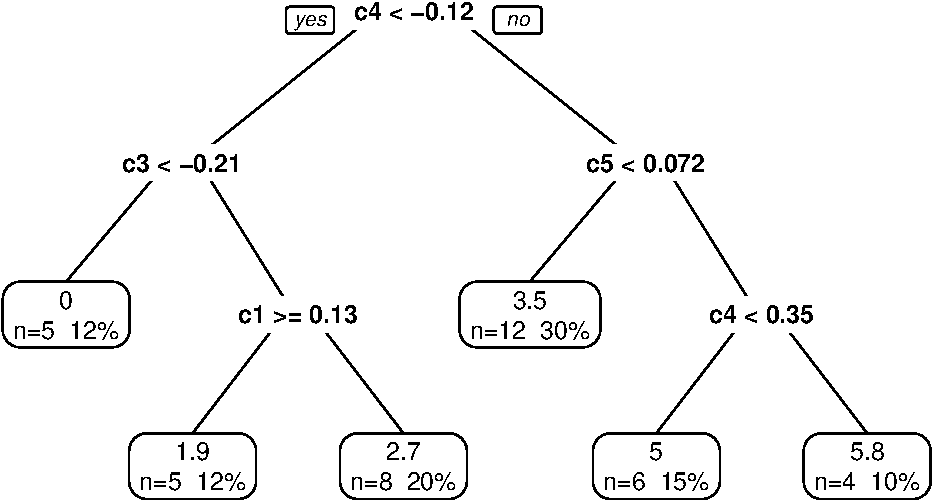
\includegraphics{Figs/plot_tree_prp-1.pdf}
\caption{Figure: Regression tree on mean clusters. Fitted regression
tree on the mean cluster data, predicting the log time classes.
Splitting points are on the mean cluster values.}
\end{figure}

\begin{Shaded}
\begin{Highlighting}[]
\CommentTok{# visualize cross-validation results }
\CommentTok{# rsq.rpart(tree.reg) }
\end{Highlighting}
\end{Shaded}

Figure: Regression tree on mean clusters. Fitted regression tree on the
mean cluster data, predicting the log time classes. Splitting points are
on the mean cluster values.

Detailed information about the fitted tree is provided below \tiny

\begin{Shaded}
\begin{Highlighting}[]
\CommentTok{# detailed overview of the resulting tree}
\KeywordTok{options}\NormalTok{(}\DataTypeTok{width=}\DecValTok{200}\NormalTok{)}
\KeywordTok{print}\NormalTok{(tree.reg)}
\end{Highlighting}
\end{Shaded}

\begin{verbatim}
n= 40 

node), split, n, deviance, yval
      * denotes terminal node

 1) root 40 1.111047e+02 3.174622  
   2) c4< -0.1174939 18 2.310447e+01 1.743756  
     4) c3< -0.2081362 5 0.000000e+00 0.000000 *
     5) c3>=-0.2081362 13 2.053563e+00 2.414432  
      10) c1>=0.1331057 5 2.465190e-31 1.945910 *
      11) c1< 0.1331057 8 2.700232e-01 2.707258 *
   3) c4>=-0.1174939 22 2.099513e+01 4.345331  
     6) c5< 0.07192204 12 1.384347e+00 3.543160 *
     7) c5>=0.07192204 10 2.622937e+00 5.307937  
      14) c4< 0.3463259 6 8.743124e-01 4.966506 *
      15) c4>=0.3463259 4 0.000000e+00 5.820083 *
\end{verbatim}

\begin{Shaded}
\begin{Highlighting}[]
\KeywordTok{summary}\NormalTok{(tree.reg)}
\end{Highlighting}
\end{Shaded}

\begin{verbatim}
Call:
rpart(formula = formula.reg, data = treedata.mean, method = "anova", 
    control = rpart.control(minsplit = 6, minbucket = 2, cp = 0.01))
  n= 40 

          CP nsplit  rel error    xerror      xstd
1 0.60308067      0 1.00000000 1.0583482 0.2114697
2 0.18946910      1 0.39691933 0.8756264 0.2911604
3 0.15289945      2 0.20745023 0.6849442 0.2942429
4 0.01605279      3 0.05455078 0.4369677 0.2245846
5 0.01573853      4 0.03849799 0.4365983 0.2243070
6 0.01000000      5 0.02275946 0.3595878 0.1860993

Variable importance
c4 c5 c1 c3 c6 c2 
27 19 19 15 12  8 

Node number 1: 40 observations,    complexity param=0.6030807
  mean=3.174622, MSE=2.777617 
  left son=2 (18 obs) right son=3 (22 obs)
  Primary splits:
      c4 < -0.1174939   to the left,  improve=0.6030807, (0 missing)
      c1 < -0.07537026  to the right, improve=0.5729499, (0 missing)
      c5 < -0.008508656 to the left,  improve=0.5487412, (0 missing)
      c3 < -0.2829117   to the left,  improve=0.5183388, (0 missing)
      c6 < -0.149531    to the left,  improve=0.3184694, (0 missing)
  Surrogate splits:
      c1 < -0.07537026  to the right, agree=0.850, adj=0.667, (0 split)
      c5 < -0.0625688   to the left,  agree=0.800, adj=0.556, (0 split)
      c6 < -0.149531    to the left,  agree=0.750, adj=0.444, (0 split)
      c2 < 0.07279386   to the right, agree=0.675, adj=0.278, (0 split)
      c3 < -0.2829117   to the left,  agree=0.675, adj=0.278, (0 split)

Node number 2: 18 observations,    complexity param=0.1894691
  mean=1.743756, MSE=1.283582 
  left son=4 (5 obs) right son=5 (13 obs)
  Primary splits:
      c3 < -0.2081362   to the left,  improve=0.9111184, (0 missing)
      c5 < -0.1122942   to the right, improve=0.5991729, (0 missing)
      c1 < 0.09730379   to the right, improve=0.5785906, (0 missing)
      c4 < -0.1838753   to the left,  improve=0.4737815, (0 missing)
      c6 < -0.01908181  to the left,  improve=0.3296556, (0 missing)
  Surrogate splits:
      c4 < -0.1838753   to the left,  agree=0.889, adj=0.6, (0 split)
      c5 < -0.1122942   to the right, agree=0.889, adj=0.6, (0 split)
      c1 < 0.3351088    to the right, agree=0.833, adj=0.4, (0 split)

Node number 3: 22 observations,    complexity param=0.1528994
  mean=4.345331, MSE=0.9543241 
  left son=6 (12 obs) right son=7 (10 obs)
  Primary splits:
      c5 < 0.07192204   to the left,  improve=0.8091327, (0 missing)
      c4 < 0.1840943    to the left,  improve=0.7540271, (0 missing)
      c1 < -0.1437557   to the right, improve=0.6642991, (0 missing)
      c3 < -0.08194432  to the right, improve=0.6127738, (0 missing)
      c6 < 0.007982308  to the right, improve=0.5246106, (0 missing)
  Surrogate splits:
      c4 < 0.1840943    to the left,  agree=0.955, adj=0.9, (0 split)
      c1 < -0.1936876   to the right, agree=0.909, adj=0.8, (0 split)
      c3 < -0.08194432  to the right, agree=0.864, adj=0.7, (0 split)
      c6 < 0.007982308  to the right, agree=0.864, adj=0.7, (0 split)
      c2 < -0.07256249  to the right, agree=0.727, adj=0.4, (0 split)

Node number 4: 5 observations
  mean=0, MSE=0 

Node number 5: 13 observations,    complexity param=0.01605279
  mean=2.414432, MSE=0.1579664 
  left son=10 (5 obs) right son=11 (8 obs)
  Primary splits:
      c1 < 0.1331057    to the right, improve=0.8685099, (0 missing)
      c2 < 0.02364916   to the right, improve=0.8685099, (0 missing)
      c3 < 0.06868251   to the left,  improve=0.7242745, (0 missing)
      c6 < -0.09746977  to the left,  improve=0.7242745, (0 missing)
      c5 < -0.1383548   to the right, improve=0.4701461, (0 missing)
  Surrogate splits:
      c2 < 0.02364916   to the right, agree=1.000, adj=1.0, (0 split)
      c3 < 0.06868251   to the left,  agree=0.923, adj=0.8, (0 split)
      c6 < -0.2167742   to the left,  agree=0.923, adj=0.8, (0 split)
      c4 < -0.153395    to the left,  agree=0.846, adj=0.6, (0 split)
      c5 < -0.1383548   to the right, agree=0.846, adj=0.6, (0 split)

Node number 6: 12 observations
  mean=3.54316, MSE=0.1153623 

Node number 7: 10 observations,    complexity param=0.01573853
  mean=5.307937, MSE=0.2622937 
  left son=14 (6 obs) right son=15 (4 obs)
  Primary splits:
      c4 < 0.3463259    to the left,  improve=0.6666667, (0 missing)
      c5 < 0.2491244    to the left,  improve=0.6666667, (0 missing)
      c6 < -0.1217972   to the left,  improve=0.2500000, (0 missing)
      c3 < -0.0328633   to the right, improve=0.2500000, (0 missing)
      c1 < -0.247735    to the left,  improve=0.1666667, (0 missing)
  Surrogate splits:
      c5 < 0.2821139    to the left,  agree=0.9, adj=0.75, (0 split)
      c1 < -0.2249667   to the left,  agree=0.7, adj=0.25, (0 split)
      c2 < -0.06371928  to the left,  agree=0.7, adj=0.25, (0 split)
      c3 < -0.1376999   to the right, agree=0.7, adj=0.25, (0 split)
      c6 < -0.06444851  to the left,  agree=0.7, adj=0.25, (0 split)

Node number 10: 5 observations
  mean=1.94591, MSE=4.930381e-32 

Node number 11: 8 observations
  mean=2.707258, MSE=0.0337529 

Node number 14: 6 observations
  mean=4.966506, MSE=0.1457187 

Node number 15: 4 observations
  mean=5.820083, MSE=0 
\end{verbatim}

\begin{Shaded}
\begin{Highlighting}[]
\KeywordTok{printcp}\NormalTok{(tree.reg)}
\end{Highlighting}
\end{Shaded}

\begin{verbatim}

Regression tree:
rpart(formula = formula.reg, data = treedata.mean, method = "anova", 
    control = rpart.control(minsplit = 6, minbucket = 2, cp = 0.01))

Variables actually used in tree construction:
[1] c1 c3 c4 c5

Root node error: 111.1/40 = 2.7776

n= 40 

        CP nsplit rel error  xerror    xstd
1 0.603081      0  1.000000 1.05835 0.21147
2 0.189469      1  0.396919 0.87563 0.29116
3 0.152899      2  0.207450 0.68494 0.29424
4 0.016053      3  0.054551 0.43697 0.22458
5 0.015739      4  0.038498 0.43660 0.22431
6 0.010000      5  0.022759 0.35959 0.18610
\end{verbatim}

\begin{Shaded}
\begin{Highlighting}[]
\NormalTok{tree.reg$frame}
\end{Highlighting}
\end{Shaded}

\begin{verbatim}
      var  n wt          dev     yval  complexity ncompete nsurrogate
1      c4 40 40 1.111047e+02 3.174622 0.603080672        4          5
2      c3 18 18 2.310447e+01 1.743756 0.189469098        4          3
4  <leaf>  5  5 0.000000e+00 0.000000 0.010000000        0          0
5      c1 13 13 2.053563e+00 2.414432 0.016052788        4          5
10 <leaf>  5  5 2.465190e-31 1.945910 0.010000000        0          0
11 <leaf>  8  8 2.700232e-01 2.707258 0.010000000        0          0
3      c5 22 22 2.099513e+01 4.345331 0.152899447        4          5
6  <leaf> 12 12 1.384347e+00 3.543160 0.007176239        0          0
7      c4 10 10 2.622937e+00 5.307937 0.015738533        4          5
14 <leaf>  6  6 8.743124e-01 4.966506 0.010000000        0          0
15 <leaf>  4  4 0.000000e+00 5.820083 0.010000000        0          0
\end{verbatim}

\begin{Shaded}
\begin{Highlighting}[]
\KeywordTok{options}\NormalTok{(}\DataTypeTok{width=}\DecValTok{75}\NormalTok{)}
\end{Highlighting}
\end{Shaded}

\normalsize

Only a subset of all mean clusters is used in the regression tree:

\begin{Shaded}
\begin{Highlighting}[]
\CommentTok{# variables used for splitting in the decision tree}
\NormalTok{tree.nodes <-}\StringTok{ }\NormalTok{(tree.reg$frame)$var}
\NormalTok{tree.nodes <-}\StringTok{ }\NormalTok{tree.nodes[tree.nodes !=}\StringTok{ "<leaf>"}\NormalTok{]}
\NormalTok{tree.vars <-}\StringTok{ }\KeywordTok{as.character}\NormalTok{(}\KeywordTok{sort}\NormalTok{(}\KeywordTok{unique}\NormalTok{(tree.nodes)))}
\KeywordTok{rm}\NormalTok{(tree.nodes)}
\CommentTok{# variables used for splitting decisions in tree}
\KeywordTok{print}\NormalTok{(tree.vars)}
\end{Highlighting}
\end{Shaded}

\begin{verbatim}
[1] "c1" "c3" "c4" "c5"
\end{verbatim}

\subsection{Leave-one-out cross
validation}\label{leave-one-out-cross-validation}

A leave-one-out approach was used to test the robustness of the
predicted time classes and predictive performance: For each sample
(\(N_{s}=40\) mice), the regression tree was generated under the
exclusion of data from the sample, with subsequent prediction on the
left out test data

\begin{Shaded}
\begin{Highlighting}[]
\CommentTok{# in total 40 cross validations (individual mice are not followed through time)}
\NormalTok{trees.test <-}\StringTok{ }\KeywordTok{vector}\NormalTok{(}\StringTok{"list"}\NormalTok{, }\DataTypeTok{length=}\NormalTok{Nr*Nt)  }\CommentTok{# fitted trees}
\NormalTok{pred.test.log <-}\StringTok{ }\KeywordTok{rep}\NormalTok{(}\OtherTok{NA}\NormalTok{, }\DataTypeTok{length=}\NormalTok{Nr*Nt)}
\NormalTok{for (k in }\DecValTok{1}\NormalTok{:(Nr*Nt))\{}
  \CommentTok{# delete the k index}
  \NormalTok{idx.subset <-}\StringTok{ }\DecValTok{1}\NormalTok{:(Nr*Nt)}
  \NormalTok{idx.subset <-}\StringTok{ }\NormalTok{idx.subset[-k]}
  
  \CommentTok{# fit tree with the subset}
  \NormalTok{t.test <-}\StringTok{ }\KeywordTok{rpart}\NormalTok{(}\DataTypeTok{formula=}\NormalTok{formula.reg, }
                  \DataTypeTok{data=}\NormalTok{treedata.mean[idx.subset, ], }
                  \DataTypeTok{method=}\StringTok{"anova"}\NormalTok{, }
                  \DataTypeTok{control=}\KeywordTok{rpart.control}\NormalTok{(}\DataTypeTok{minsplit=}\DecValTok{6}\NormalTok{, }\DataTypeTok{minbucket=}\DecValTok{2}\NormalTok{, }\DataTypeTok{cp=}\FloatTok{0.01}\NormalTok{))  }
  \NormalTok{trees.test[[k]] <-}\StringTok{ }\NormalTok{t.test}
  
  \CommentTok{# prediction on left out sample}
  \NormalTok{pred.test.log[k] <-}\StringTok{ }\KeywordTok{predict}\NormalTok{(t.test, }\DataTypeTok{newdata=}\NormalTok{treedata.mean[k,], }\DataTypeTok{type=}\StringTok{"vector"}\NormalTok{)}
\NormalTok{\}}
\CommentTok{# transformation to time in [h]}
\NormalTok{pred.test <-}\StringTok{ }\KeywordTok{log_transform_back}\NormalTok{( pred.test.log )}

\NormalTok{plot_cross_validation <-}\StringTok{ }\NormalTok{function()\{}
\CommentTok{# plot the log prediction and error}
  \KeywordTok{par}\NormalTok{(}\DataTypeTok{mfrow=}\KeywordTok{c}\NormalTok{(}\DecValTok{1}\NormalTok{,}\DecValTok{2}\NormalTok{))}
  \KeywordTok{plot}\NormalTok{(}\KeywordTok{log_transform}\NormalTok{(BDLsamples$time), }\KeywordTok{log_transform}\NormalTok{(pred.test),}
       \DataTypeTok{main=}\StringTok{"Leave one out cross validation"}\NormalTok{,}
       \DataTypeTok{xlim=}\KeywordTok{c}\NormalTok{(}\DecValTok{0}\NormalTok{,}\DecValTok{7}\NormalTok{), }\DataTypeTok{ylim=}\KeywordTok{c}\NormalTok{(}\DecValTok{0}\NormalTok{,}\DecValTok{7}\NormalTok{),}
       \DataTypeTok{xlab=}\StringTok{"log(time_exp)"}\NormalTok{,}
       \DataTypeTok{ylab=}\StringTok{"log(time_pre)"}\NormalTok{)}
  \KeywordTok{abline}\NormalTok{(}\DataTypeTok{a=}\DecValTok{0}\NormalTok{, }\DataTypeTok{b=}\DecValTok{1}\NormalTok{, }\DataTypeTok{col=}\StringTok{"gray"}\NormalTok{)}
  \KeywordTok{textxy}\NormalTok{(}\KeywordTok{log_transform}\NormalTok{(BDLsamples$time), }\KeywordTok{log_transform}\NormalTok{(pred.test), }
         \DecValTok{1}\NormalTok{:(Nr*Nt), }\DataTypeTok{col=}\StringTok{"black"}\NormalTok{, }\DataTypeTok{cex=}\FloatTok{0.6}\NormalTok{)}
  
  \KeywordTok{plot}\NormalTok{(}\KeywordTok{log_transform}\NormalTok{(BDLsamples$time), }
       \KeywordTok{log_transform}\NormalTok{(BDLsamples$time)-}\KeywordTok{log_transform}\NormalTok{(pred.test),}
       \DataTypeTok{main=}\StringTok{"Prediction error"}\NormalTok{,}
       \DataTypeTok{xlab=}\StringTok{"log(time_exp)"}\NormalTok{,}
       \DataTypeTok{ylab=}\StringTok{"log(time_exp)-log(time_pre)"}\NormalTok{,}
       \DataTypeTok{xlim=}\KeywordTok{c}\NormalTok{(}\DecValTok{0}\NormalTok{,}\DecValTok{7}\NormalTok{), }\DataTypeTok{ylim=}\KeywordTok{c}\NormalTok{(-}\FloatTok{1.5}\NormalTok{, }\FloatTok{1.5}\NormalTok{))}
  \KeywordTok{abline}\NormalTok{(}\DataTypeTok{a=}\DecValTok{0}\NormalTok{, }\DataTypeTok{b=}\DecValTok{0}\NormalTok{, }\DataTypeTok{col=}\StringTok{"gray"}\NormalTok{)}
  \KeywordTok{textxy}\NormalTok{(}\KeywordTok{log_transform}\NormalTok{(BDLsamples$time), }
         \KeywordTok{log_transform}\NormalTok{(BDLsamples$time)-}\KeywordTok{log_transform}\NormalTok{(pred.test), }
         \DecValTok{1}\NormalTok{:(Nr*Nt), }\DataTypeTok{col=}\StringTok{"black"}\NormalTok{, }\DataTypeTok{cex=}\FloatTok{0.6}\NormalTok{)}
  \KeywordTok{par}\NormalTok{(}\DataTypeTok{mfrow=}\KeywordTok{c}\NormalTok{(}\DecValTok{1}\NormalTok{,}\DecValTok{1}\NormalTok{))  }
\NormalTok{\}}
\end{Highlighting}
\end{Shaded}

\begin{Shaded}
\begin{Highlighting}[]
\KeywordTok{plot_cross_validation}\NormalTok{()}
\end{Highlighting}
\end{Shaded}

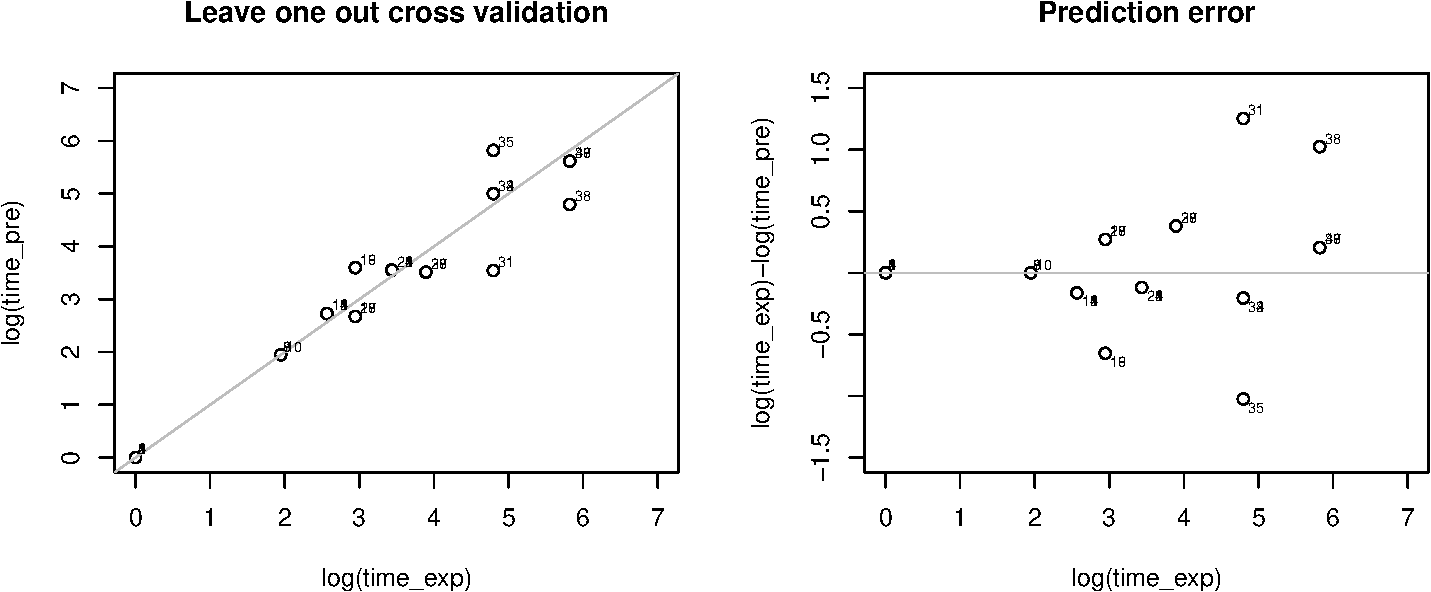
\includegraphics{Figs/plot_tree_cv-1.pdf}

Figure: Cross validation predictions. Predictions on the left out data
set with the fitted tree.

\emph{Results:} All time points of the left-out data are predicted close
to their actual time.

\subsection{Prediction on trainings
data}\label{prediction-on-trainings-data}

Predict data with the tree: Here the time class leaves based on the mean
cluster data. The regression tree predicts log classes, which are
back-transformed to time in {[}h{]}. Here we test how good the tree
performing on the trainings data set, i.e.~the mean cluster data.
Predictons are evaluated based on the distance between the predicted and
the experimental time classes based on the following distance measure on
log scale

\begin{Shaded}
\begin{Highlighting}[]
\CommentTok{# L2 (euclidian) distance measurement on the log transformed data. }
\CommentTok{# Analog to the distance measurement in fitting the regression tree.}
\NormalTok{log_distance <-}\StringTok{ }\NormalTok{function(d1, d2)\{}
  \CommentTok{# sums over all the distances of the samples in log space}
  \NormalTok{log_rmsd <-}\StringTok{ }\KeywordTok{sqrt}\NormalTok{(}\KeywordTok{sum}\NormalTok{( (}\KeywordTok{log_transform}\NormalTok{(d1)-}\KeywordTok{log_transform}\NormalTok{(d2) )^}\DecValTok{2} \NormalTok{))/}\KeywordTok{length}\NormalTok{(d1)}
  \KeywordTok{return}\NormalTok{(log_rmsd)}
\NormalTok{\}}
\end{Highlighting}
\end{Shaded}

Prediction on trainings data

\begin{Shaded}
\begin{Highlighting}[]
\CommentTok{# mean cluster predictions}
\NormalTok{pred.mean.log <-}\StringTok{ }\KeywordTok{predict}\NormalTok{(tree.reg, }\DataTypeTok{newdata=}\NormalTok{treedata.mean, }\DataTypeTok{type=}\StringTok{"vector"}\NormalTok{)}
\CommentTok{# transformation to time in [h]}
\NormalTok{pred.mean <-}\StringTok{ }\KeywordTok{log_transform_back}\NormalTok{( pred.mean.log )}

\CommentTok{# Distance calculation (predicted to experimental)}
\NormalTok{dist.mean.all <-}\StringTok{ }\NormalTok{treedata.mean$logtime -}\StringTok{ }\NormalTok{pred.mean.log}
\NormalTok{dist.mean <-}\StringTok{ }\KeywordTok{log_distance}\NormalTok{(pred.mean, BDLsamples$time)}

\CommentTok{# plot predicted ~ experimentell}
\NormalTok{plot_mean_prediction <-}\StringTok{ }\NormalTok{function()\{}
  \KeywordTok{par}\NormalTok{(}\DataTypeTok{mfrow=}\KeywordTok{c}\NormalTok{(}\DecValTok{1}\NormalTok{,}\DecValTok{2}\NormalTok{))}
  \KeywordTok{plot}\NormalTok{(BDLsamples$time, pred.mean, }\DataTypeTok{pch=}\DecValTok{15}\NormalTok{, }\DataTypeTok{col=}\KeywordTok{rgb}\NormalTok{(}\DecValTok{0}\NormalTok{,}\DecValTok{0}\NormalTok{,}\DecValTok{1}\NormalTok{, }\FloatTok{0.2}\NormalTok{), }
       \DataTypeTok{main=}\StringTok{"Regression Tree:}\CharTok{\textbackslash{}n}\StringTok{Predicted ~ experimentell time"}\NormalTok{,}
       \DataTypeTok{xlab=}\StringTok{"experimentell time [h]"}\NormalTok{, }\DataTypeTok{ylab=}\StringTok{"predicted time [h]"}\NormalTok{)}
  \KeywordTok{abline}\NormalTok{(}\DataTypeTok{a=}\DecValTok{0}\NormalTok{, }\DataTypeTok{b=}\DecValTok{1}\NormalTok{, }\DataTypeTok{col=}\KeywordTok{rgb}\NormalTok{(}\FloatTok{0.5}\NormalTok{,}\FloatTok{0.5}\NormalTok{,}\FloatTok{0.5}\NormalTok{,}\FloatTok{0.5}\NormalTok{))}
  \KeywordTok{hist}\NormalTok{(dist.mean.all, }\DataTypeTok{breaks=}\KeywordTok{seq}\NormalTok{(}\DataTypeTok{from=}\NormalTok{-}\FloatTok{1.05}\NormalTok{, }\DataTypeTok{to=}\FloatTok{1.05}\NormalTok{, }\DataTypeTok{by=}\FloatTok{0.1}\NormalTok{), }
       \DataTypeTok{main=}\StringTok{"Histogram prediction error:}\CharTok{\textbackslash{}n}\StringTok{mean cluster data"}\NormalTok{,}
       \DataTypeTok{col=}\KeywordTok{rgb}\NormalTok{(}\FloatTok{0.5}\NormalTok{,}\FloatTok{0.5}\NormalTok{,}\FloatTok{0.5}\NormalTok{,}\FloatTok{0.5}\NormalTok{),}
       \DataTypeTok{xlab=}\StringTok{"logtime(exp)-logtime(pred)"}\NormalTok{)}
  \KeywordTok{par}\NormalTok{(}\DataTypeTok{mfrow=}\KeywordTok{c}\NormalTok{(}\DecValTok{1}\NormalTok{,}\DecValTok{1}\NormalTok{))  }
\NormalTok{\}}
\CommentTok{# plot to file}
\KeywordTok{pdf}\NormalTok{(}\KeywordTok{file.path}\NormalTok{(resultsPath, }\StringTok{'decision_tree'}\NormalTok{, }\StringTok{"prediction_mean.pdf"}\NormalTok{), }
    \DataTypeTok{width=}\DecValTok{10}\NormalTok{, }\DataTypeTok{height=}\DecValTok{5}\NormalTok{, }\DataTypeTok{pointsize=}\DecValTok{12}\NormalTok{)  }
\KeywordTok{plot_mean_prediction}\NormalTok{()}
\KeywordTok{invisible}\NormalTok{(}\KeywordTok{dev.off}\NormalTok{())}
\end{Highlighting}
\end{Shaded}

\begin{Shaded}
\begin{Highlighting}[]
\KeywordTok{plot_mean_prediction}\NormalTok{()}
\end{Highlighting}
\end{Shaded}

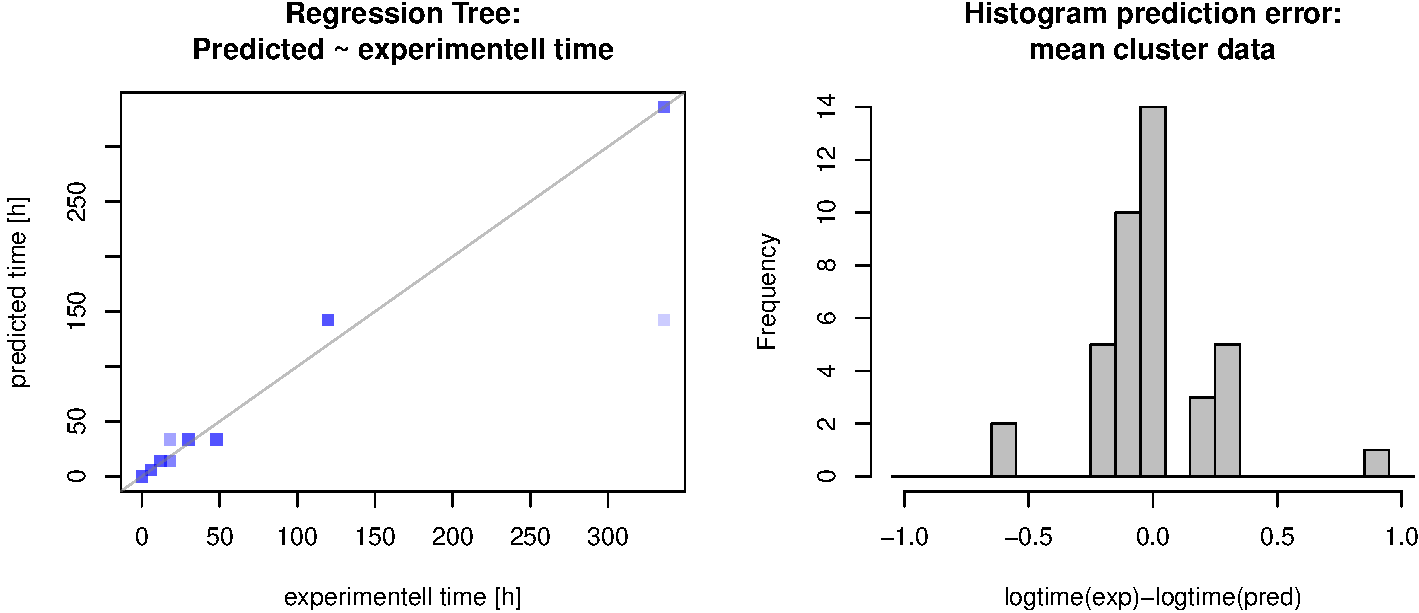
\includegraphics{Figs/plot_mean_prediction-1.pdf}

Figure: Predictions on mean cluster data. Predictions using the mean
cluster data. This is the trainings data and results in the best
performing tree.

The ranges of the predicted classes by the regression trees can be
calculated based on the split points on log scale. These provides the
information which time points would be classified in which class in the
regression tree.

\begin{Shaded}
\begin{Highlighting}[]
\NormalTok{calculate_node_ranges <-}\StringTok{ }\NormalTok{function()\{}
  \CommentTok{# classes via predicted classes for cluster data}
  \NormalTok{node_levels <-}\StringTok{ }\KeywordTok{levels}\NormalTok{(}\KeywordTok{as.factor}\NormalTok{(pred.mean))}
  \CommentTok{# These are the predicted classes}
  \NormalTok{node_classes <-}\StringTok{ }\KeywordTok{round}\NormalTok{(}\KeywordTok{as.numeric}\NormalTok{(node_levels), }\DataTypeTok{digits=}\DecValTok{1}\NormalTok{)}
  
  \CommentTok{# get the intervals of the time classes}
  \NormalTok{node_mean <-}\StringTok{ }\KeywordTok{as.numeric}\NormalTok{(}\KeywordTok{levels}\NormalTok{(}\KeywordTok{as.factor}\NormalTok{(pred.mean.log)))}
  \NormalTok{node_midpoints <-}\StringTok{ }\NormalTok{(node_mean[}\DecValTok{2}\NormalTok{:}\KeywordTok{length}\NormalTok{(node_mean)]+node_mean[}\DecValTok{1}\NormalTok{:(}\KeywordTok{length}\NormalTok{(node_mean)-}\DecValTok{1}\NormalTok{)])/}\DecValTok{2}
  \CommentTok{# minimum of range}
  \NormalTok{node_min <-}\StringTok{ }\NormalTok{node_mean}
  \NormalTok{node_min[}\DecValTok{2}\NormalTok{:}\KeywordTok{length}\NormalTok{(node_min)] <-}\StringTok{ }\NormalTok{node_midpoints}
  \CommentTok{# maximum of range}
  \NormalTok{node_max <-}\StringTok{ }\NormalTok{node_mean}
  \NormalTok{node_max[}\DecValTok{1}\NormalTok{:(}\KeywordTok{length}\NormalTok{(node_min)-}\DecValTok{1}\NormalTok{)] <-}\StringTok{ }\NormalTok{node_midpoints}
  \CommentTok{# ranges in log scale}
  \NormalTok{node_ranges.log <-}\StringTok{ }\KeywordTok{data.frame}\NormalTok{(node_mean, node_min, node_max)}
  
  \NormalTok{node_ranges <-}\StringTok{ }\KeywordTok{data.frame}\NormalTok{(}\DataTypeTok{mean=}\KeywordTok{log_transform_back}\NormalTok{(node_mean), }
                            \DataTypeTok{min=}\KeywordTok{log_transform_back}\NormalTok{(node_min),}
                            \DataTypeTok{max=}\KeywordTok{log_transform_back}\NormalTok{(node_max))}
  \KeywordTok{rownames}\NormalTok{(node_ranges) <-}\StringTok{ }\KeywordTok{paste}\NormalTok{(}\StringTok{"class"}\NormalTok{, }\DecValTok{1}\NormalTok{:}\KeywordTok{nrow}\NormalTok{(node_ranges))}
  \KeywordTok{return}\NormalTok{(node_ranges)}
\NormalTok{\}}

\CommentTok{# predicted time classes by decision tree}
\NormalTok{node_ranges <-}\StringTok{ }\KeywordTok{calculate_node_ranges}\NormalTok{()}
\KeywordTok{print}\NormalTok{(}\KeywordTok{round}\NormalTok{(node_ranges, }\DataTypeTok{digits=}\DecValTok{1}\NormalTok{))}
\end{Highlighting}
\end{Shaded}

\begin{verbatim}
         mean   min   max
class 1   0.0   0.0   1.6
class 2   6.0   1.6   9.2
class 3  14.0   9.2  21.8
class 4  33.6  21.8  69.4
class 5 142.5  69.4 218.9
class 6 336.0 218.9 336.0
\end{verbatim}

\subsection{Test data for evaluation}\label{test-data-for-evaluation}

\subsubsection{Single factor per
cluster}\label{single-factor-per-cluster}

Now the data set consisting of all single factor combinations from the
clusters is created. These are used to evaluate the fitted regression
tree.

\begin{Shaded}
\begin{Highlighting}[]
\CommentTok{# names of factors in the clusters}
\NormalTok{cluster_names <-}\StringTok{ }\KeywordTok{paste}\NormalTok{(}\StringTok{'c'}\NormalTok{, }\DecValTok{1}\NormalTok{:Ngroups, }\DataTypeTok{sep=}\StringTok{""}\NormalTok{)}
\NormalTok{cluster.factors <-}\StringTok{ }\KeywordTok{vector}\NormalTok{(}\StringTok{"list"}\NormalTok{, }\DataTypeTok{length=}\NormalTok{Ngroups)}
\NormalTok{groups <-}\StringTok{ }\NormalTok{(hclust.res$ys3)$groups  }\CommentTok{# get the ys3 groups}
\NormalTok{for (k in }\DecValTok{1}\NormalTok{:Ngroups)\{}
  \NormalTok{cluster.factors[[k]] <-}\StringTok{ }\KeywordTok{as.character}\NormalTok{(}\KeywordTok{names}\NormalTok{(groups[groups==k]))}
\NormalTok{\}}
\KeywordTok{names}\NormalTok{(cluster.factors) <-}\StringTok{ }\NormalTok{cluster_names}

\CommentTok{# create data.frame of all single combinations from clusters}
\NormalTok{single.combinations <-}\StringTok{ }\KeywordTok{expand.grid}\NormalTok{(cluster.factors, }\DataTypeTok{stringsAsFactors=}\OtherTok{TRUE}\NormalTok{)}
\KeywordTok{names}\NormalTok{(single.combinations) <-}\StringTok{ }\KeywordTok{names}\NormalTok{(cluster.factors)}
\CommentTok{# number of single combinations}
\NormalTok{Nsingle <-}\StringTok{ }\KeywordTok{nrow}\NormalTok{(single.combinations)}

\CommentTok{# create all single factor data}
\KeywordTok{print}\NormalTok{(}\StringTok{"Calculating single factor data (~ 3min) ... "}\NormalTok{)}
\end{Highlighting}
\end{Shaded}

\begin{verbatim}
[1] "Calculating single factor data (~ 3min) ... "
\end{verbatim}

\begin{Shaded}
\begin{Highlighting}[]
\NormalTok{ptm <-}\StringTok{ }\KeywordTok{proc.time}\NormalTok{()  }
\NormalTok{treedata.single <-}\StringTok{ }\KeywordTok{vector}\NormalTok{(}\StringTok{"list"}\NormalTok{, Nsingle)  }\CommentTok{# list for all combinations}
\NormalTok{for (k in }\DecValTok{1}\NormalTok{:Nsingle)\{}
  \CommentTok{# ----------------------------------------------------------------}
  \CommentTok{# THIS HAS TO BE FAST (<0.005 s)}
  \CommentTok{# ----------------------------------------------------------------}
  \CommentTok{# ptm <- proc.time() # Start the clock!}
  \CommentTok{# get factor data}
  \NormalTok{tmp <-}\StringTok{ }\NormalTok{BDLdata.norm[, }\KeywordTok{t}\NormalTok{(single.combinations[k, ]) ]}
  \CommentTok{# add regression values}
  \NormalTok{tmp[}\KeywordTok{c}\NormalTok{(}\StringTok{"class"}\NormalTok{, }\StringTok{"logtime"}\NormalTok{)] <-}\StringTok{ }\NormalTok{treedata.mean[ }\KeywordTok{c}\NormalTok{(}\StringTok{"class"}\NormalTok{, }\StringTok{"logtime"}\NormalTok{)]}
  \CommentTok{# add factor fields }
  \NormalTok{tmp[, }\KeywordTok{paste}\NormalTok{(cluster_names, }\StringTok{'.id'}\NormalTok{, }\DataTypeTok{sep=}\StringTok{""}\NormalTok{)] <-}\StringTok{ }\NormalTok{single.combinations[k,]}
  \KeywordTok{colnames}\NormalTok{(tmp) <-}\StringTok{ }\KeywordTok{c}\NormalTok{(cluster_names, }\StringTok{'class'}\NormalTok{, }\StringTok{'logtime'}\NormalTok{, }\KeywordTok{paste}\NormalTok{(cluster_names, }\StringTok{'.id'}\NormalTok{, }\DataTypeTok{sep=}\StringTok{""}\NormalTok{))}
  \CommentTok{# store data }
  \NormalTok{treedata.single[[k]] <-}\StringTok{ }\NormalTok{tmp}
  \CommentTok{# if (k%%500 == 0)\{print(k)\} }
  \CommentTok{# print(proc.time()-ptm)  # Stop the clock}
\NormalTok{\}}
\CommentTok{# Stop the clock}
\KeywordTok{rm}\NormalTok{(tmp,k)}
\KeywordTok{print}\NormalTok{(}\KeywordTok{proc.time}\NormalTok{() -}\StringTok{ }\NormalTok{ptm)}
\end{Highlighting}
\end{Shaded}

\begin{verbatim}
   user  system elapsed 
119.374   0.120 119.473 
\end{verbatim}

\begin{Shaded}
\begin{Highlighting}[]
\CommentTok{# which factor combinations only use genes}
\NormalTok{factor_is_gene <-}\StringTok{ }\NormalTok{BDLfactors$ftype %in%}\StringTok{ }\KeywordTok{c}\NormalTok{(}\StringTok{"GE_ADME"}\NormalTok{, }\StringTok{"GE_Cytokines"}\NormalTok{, }\StringTok{"GE_Fibrosis"}\NormalTok{)}
\KeywordTok{names}\NormalTok{(factor_is_gene) <-}\StringTok{ }\NormalTok{BDLfactors$id}
\CommentTok{# vector for lookup if only genes were used}
\NormalTok{gene_only.single <-}\StringTok{ }\KeywordTok{vector}\NormalTok{(}\StringTok{"logical"}\NormalTok{, Nsingle)}
\NormalTok{for (k in }\DecValTok{1}\NormalTok{:Nsingle)\{}
  \NormalTok{gene_only.single[k] <-}\StringTok{ }\KeywordTok{all}\NormalTok{(factor_is_gene[}\KeywordTok{t}\NormalTok{(single.combinations[k,])])}
\NormalTok{\}}
\KeywordTok{rm}\NormalTok{(k)}
\end{Highlighting}
\end{Shaded}

The single factor data was created consisting of 88572 combinations.

\subsubsection{Double factor per
cluster}\label{double-factor-per-cluster}

Create a sample of double combinations from the various clusters.

\begin{Shaded}
\begin{Highlighting}[]
\KeywordTok{print}\NormalTok{(}\StringTok{"Calculating double factor data (~ 1min) ... "}\NormalTok{)}
\end{Highlighting}
\end{Shaded}

\begin{verbatim}
[1] "Calculating double factor data (~ 1min) ... "
\end{verbatim}

\begin{Shaded}
\begin{Highlighting}[]
\NormalTok{ptm <-}\StringTok{ }\KeywordTok{proc.time}\NormalTok{()}
\KeywordTok{set.seed}\NormalTok{(}\DecValTok{123456}\NormalTok{)}
\NormalTok{Ndouble <-}\StringTok{ }\DecValTok{10000}
\NormalTok{treedata.double <-}\StringTok{ }\KeywordTok{vector}\NormalTok{(}\StringTok{"list"}\NormalTok{, Ndouble)  }\CommentTok{# list for sampled double combinations}
\NormalTok{for (k in }\DecValTok{1}\NormalTok{:Ndouble)\{}
  \CommentTok{# sample from the 4 clusters without replacement}
  \NormalTok{n1 =}\StringTok{ }\KeywordTok{sample}\NormalTok{(cluster.factors[[}\DecValTok{1}\NormalTok{]], }\DecValTok{2}\NormalTok{, }\DataTypeTok{replace=}\OtherTok{FALSE}\NormalTok{)  }
  \NormalTok{n2 =}\StringTok{ }\KeywordTok{sample}\NormalTok{(cluster.factors[[}\DecValTok{2}\NormalTok{]], }\DecValTok{2}\NormalTok{, }\DataTypeTok{replace=}\OtherTok{FALSE}\NormalTok{)  }
  \NormalTok{n3 =}\StringTok{ }\KeywordTok{sample}\NormalTok{(cluster.factors[[}\DecValTok{3}\NormalTok{]], }\DecValTok{2}\NormalTok{, }\DataTypeTok{replace=}\OtherTok{FALSE}\NormalTok{)  }
  \NormalTok{n4 =}\StringTok{ }\KeywordTok{sample}\NormalTok{(cluster.factors[[}\DecValTok{4}\NormalTok{]], }\DecValTok{2}\NormalTok{, }\DataTypeTok{replace=}\OtherTok{FALSE}\NormalTok{)  }
  \NormalTok{n5 =}\StringTok{ }\KeywordTok{sample}\NormalTok{(cluster.factors[[}\DecValTok{5}\NormalTok{]], }\DecValTok{2}\NormalTok{, }\DataTypeTok{replace=}\OtherTok{FALSE}\NormalTok{)  }
  \NormalTok{n6 =}\StringTok{ }\KeywordTok{sample}\NormalTok{(cluster.factors[[}\DecValTok{6}\NormalTok{]], }\DecValTok{2}\NormalTok{, }\DataTypeTok{replace=}\OtherTok{FALSE}\NormalTok{)  }
  \CommentTok{# The mean of the combination is used (handle NAs)}
  \NormalTok{tmp <-}\StringTok{ }\FloatTok{0.5} \NormalTok{*}\StringTok{ }\NormalTok{(  BDLdata.norm[, }\KeywordTok{c}\NormalTok{(n1[}\DecValTok{1}\NormalTok{], n2[}\DecValTok{1}\NormalTok{], n3[}\DecValTok{1}\NormalTok{], n4[}\DecValTok{1}\NormalTok{], n5[}\DecValTok{1}\NormalTok{], n6[}\DecValTok{1}\NormalTok{])] }
                \NormalTok{+}\StringTok{ }\NormalTok{BDLdata.norm[, }\KeywordTok{c}\NormalTok{(n1[}\DecValTok{2}\NormalTok{], n2[}\DecValTok{2}\NormalTok{], n3[}\DecValTok{2}\NormalTok{], n4[}\DecValTok{2}\NormalTok{], n5[}\DecValTok{2}\NormalTok{], n6[}\DecValTok{2}\NormalTok{])] )}
   \CommentTok{# add class and regression values}
  \NormalTok{tmp[}\KeywordTok{c}\NormalTok{(}\StringTok{"class"}\NormalTok{, }\StringTok{"logtime"}\NormalTok{)] <-}\StringTok{ }\NormalTok{treedata.mean[ }\KeywordTok{c}\NormalTok{(}\StringTok{"class"}\NormalTok{, }\StringTok{"logtime"}\NormalTok{)]}
  \CommentTok{# add factor fields }
  \NormalTok{tmp[ , }\KeywordTok{paste}\NormalTok{(cluster_names, }\StringTok{'.id'}\NormalTok{, }\DataTypeTok{sep=}\StringTok{""}\NormalTok{)] <-}\StringTok{ }\KeywordTok{data.frame}\NormalTok{(}\KeywordTok{paste}\NormalTok{(n1, }\DataTypeTok{collapse=}\StringTok{"__"}\NormalTok{), }
                                              \KeywordTok{paste}\NormalTok{(n2, }\DataTypeTok{collapse=}\StringTok{"__"}\NormalTok{),}
                                              \KeywordTok{paste}\NormalTok{(n3, }\DataTypeTok{collapse=}\StringTok{"__"}\NormalTok{),}
                                              \KeywordTok{paste}\NormalTok{(n4, }\DataTypeTok{collapse=}\StringTok{"__"}\NormalTok{),}
                                              \KeywordTok{paste}\NormalTok{(n5, }\DataTypeTok{collapse=}\StringTok{"__"}\NormalTok{),}
                                              \KeywordTok{paste}\NormalTok{(n6, }\DataTypeTok{collapse=}\StringTok{"__"}\NormalTok{))}
  \KeywordTok{colnames}\NormalTok{(tmp) <-}\StringTok{ }\KeywordTok{c}\NormalTok{(cluster_names, }\StringTok{'class'}\NormalTok{, }\StringTok{'regvalue'}\NormalTok{, }
                     \KeywordTok{paste}\NormalTok{(cluster_names, }\StringTok{'.id'}\NormalTok{, }\DataTypeTok{sep=}\StringTok{""}\NormalTok{))}
  \CommentTok{# store data}
  \NormalTok{treedata.double[[k]] <-}\StringTok{ }\NormalTok{tmp}
\NormalTok{\}}
\KeywordTok{rm}\NormalTok{(k, tmp)}
\KeywordTok{print}\NormalTok{(}\KeywordTok{proc.time}\NormalTok{() -}\StringTok{ }\NormalTok{ptm)}
\end{Highlighting}
\end{Shaded}

\begin{verbatim}
   user  system elapsed 
 33.593   0.024  33.602 
\end{verbatim}

The double factor data was created consisting of a random selection of
10\^{}\{4\} combinations.

\subsection{Prediction on test data}\label{prediction-on-test-data}

\subsubsection{Single representative
predictions}\label{single-representative-predictions}

Time class prediction with regression tree for single representative
from each cluster

\begin{Shaded}
\begin{Highlighting}[]
\KeywordTok{print}\NormalTok{(}\StringTok{"Predicting single factor data (~ 2min) ... "}\NormalTok{)}
\end{Highlighting}
\end{Shaded}

\begin{verbatim}
[1] "Predicting single factor data (~ 2min) ... "
\end{verbatim}

\begin{Shaded}
\begin{Highlighting}[]
\NormalTok{pred.single.all <-}\StringTok{ }\KeywordTok{vector}\NormalTok{(}\StringTok{"list"}\NormalTok{, }\KeywordTok{length}\NormalTok{(treedata.single))}
\NormalTok{for (k in (}\DecValTok{1}\NormalTok{:}\KeywordTok{length}\NormalTok{(treedata.single)))\{}
  \CommentTok{# prediction and back transformation  }
  \NormalTok{pred.single.all[[k]] <-}\StringTok{ }\KeywordTok{log_transform_back}\NormalTok{( }\KeywordTok{predict}\NormalTok{(tree.reg, }\DataTypeTok{newdata=}\NormalTok{treedata.single[[k]], }\DataTypeTok{method=}\StringTok{"anova"}\NormalTok{) )}
\NormalTok{\}}
\NormalTok{pred.single <-}\StringTok{ }\KeywordTok{do.call}\NormalTok{(}\StringTok{"rbind"}\NormalTok{, pred.single.all)}

\CommentTok{# distance for all predictions on single factor per cluster}
\NormalTok{dist.single <-}\StringTok{ }\KeywordTok{rep}\NormalTok{(}\OtherTok{NA}\NormalTok{, Nsingle)}
\NormalTok{for (k in }\DecValTok{1}\NormalTok{:Nsingle)\{}
  \NormalTok{dist.single[k] <-}\StringTok{ }\KeywordTok{log_distance}\NormalTok{(pred.single[k,], BDLsamples$time)}
\NormalTok{\}}
\end{Highlighting}
\end{Shaded}

\subsubsection{Double representative
predictions}\label{double-representative-predictions}

Time class prediction with regression tree for random selection of two
representatives from each clusters

\begin{Shaded}
\begin{Highlighting}[]
\KeywordTok{print}\NormalTok{(}\StringTok{"Predicting double factor data (~ 1min) ... "}\NormalTok{)}
\end{Highlighting}
\end{Shaded}

\begin{verbatim}
[1] "Predicting double factor data (~ 1min) ... "
\end{verbatim}

\begin{Shaded}
\begin{Highlighting}[]
\NormalTok{pred.double.all <-}\StringTok{ }\KeywordTok{vector}\NormalTok{(}\StringTok{"list"}\NormalTok{, }\KeywordTok{length}\NormalTok{(treedata.double))}
\NormalTok{for (k in (}\DecValTok{1}\NormalTok{:}\KeywordTok{length}\NormalTok{(treedata.double)))\{}
  \NormalTok{pred.double.all[[k]] <-}\StringTok{ }\KeywordTok{log_transform_back}\NormalTok{( }\KeywordTok{predict}\NormalTok{(tree.reg, }\DataTypeTok{newdata=}\NormalTok{treedata.double[[k]], }\DataTypeTok{method=}\StringTok{"anova"}\NormalTok{) )}
\NormalTok{\}}
\NormalTok{pred.double <-}\StringTok{ }\KeywordTok{do.call}\NormalTok{(}\StringTok{"rbind"}\NormalTok{, pred.double.all)}

\CommentTok{# distance for predictions on 2 sampled factors per cluster }
\NormalTok{dist.double <-}\StringTok{ }\KeywordTok{rep}\NormalTok{(}\OtherTok{NA}\NormalTok{, Ndouble)}
\NormalTok{for (k in }\DecValTok{1}\NormalTok{:Ndouble)\{}
  \NormalTok{dist.double[k] <-}\StringTok{ }\KeywordTok{log_distance}\NormalTok{(pred.double[k,], BDLsamples$time)}
\NormalTok{\}}
\end{Highlighting}
\end{Shaded}

\subsection{Best factor combinations}\label{best-factor-combinations}

Finding the best regression trees based on i) all single representatives
from the clusters; and ii) single representatives only consisting of
gene probes. The best is defined by minimal euclidian distance between
experimental classes and predicted classes on the log scale. The best
tree is not refitted with the respective factors in the tree, but the
mean cluster tree uses the respective factor data for prediction.

\begin{Shaded}
\begin{Highlighting}[]
\CommentTok{# Best decision tree using all factors (minimal distance)}
\NormalTok{dist.rep.best <-}\StringTok{ }\KeywordTok{min}\NormalTok{(dist.single)}
\CommentTok{# best combination of representatives for the clusters (remove duplicates)}
\NormalTok{rep.best <-}\StringTok{ }\KeywordTok{unique}\NormalTok{(single.combinations[}\KeywordTok{which}\NormalTok{(dist.single==dist.rep.best), }
                                       \KeywordTok{c}\NormalTok{(}\StringTok{"c1"}\NormalTok{, }\StringTok{"c3"}\NormalTok{, }\StringTok{"c4"}\NormalTok{, }\StringTok{"c5"}\NormalTok{)])}
\NormalTok{rep.best.idx <-}\StringTok{ }\KeywordTok{rownames}\NormalTok{(rep.best)[}\DecValTok{1}\NormalTok{]}
\CommentTok{# predictions of best representative}
\NormalTok{pred.rep.best <-}\StringTok{ }\NormalTok{pred.single[}\KeywordTok{as.numeric}\NormalTok{(rep.best.idx), ]}

\KeywordTok{print}\NormalTok{(}\StringTok{"Best single representatives for decision tree:"}\NormalTok{)}
\end{Highlighting}
\end{Shaded}

\begin{verbatim}
[1] "Best single representatives for decision tree:"
\end{verbatim}

\begin{Shaded}
\begin{Highlighting}[]
\KeywordTok{print}\NormalTok{(rep.best)}
\end{Highlighting}
\end{Shaded}

\begin{verbatim}
          c1   c3     c4    c5
16062 Cyp1a2  Fn1 S100a4 Il17a
16084 Cyp1a2 GLDH S100a4 Il17a
\end{verbatim}

\begin{Shaded}
\begin{Highlighting}[]
\KeywordTok{print}\NormalTok{(dist.rep.best)}
\end{Highlighting}
\end{Shaded}

\begin{verbatim}
[1] 0.05554854
\end{verbatim}

\begin{Shaded}
\begin{Highlighting}[]
\CommentTok{# ------------------------}
\CommentTok{# Best decision tree using only gene factors, i.e. first reduce to the gene combinations}
\NormalTok{dist.single.genes <-}\StringTok{ }\NormalTok{dist.single[gene_only.single]}
\NormalTok{single.combinations.genes <-}\StringTok{ }\NormalTok{single.combinations[gene_only.single,]}
\NormalTok{dist.gene.best <-}\StringTok{ }\KeywordTok{min}\NormalTok{(dist.single.genes)}
\CommentTok{# find best gene combination}
\NormalTok{gene.best <-}\StringTok{ }\KeywordTok{unique}\NormalTok{(single.combinations.genes[}\KeywordTok{which}\NormalTok{(dist.single.genes==dist.gene.best), }
                                              \KeywordTok{c}\NormalTok{(}\StringTok{"c1"}\NormalTok{, }\StringTok{"c3"}\NormalTok{, }\StringTok{"c4"}\NormalTok{, }\StringTok{"c5"}\NormalTok{)])}
\CommentTok{# predictions with best representative}
\NormalTok{gene.best.idx <-}\StringTok{ }\KeywordTok{rownames}\NormalTok{(gene.best)}
\NormalTok{pred.gene.best <-}\StringTok{ }\NormalTok{pred.single[}\KeywordTok{as.numeric}\NormalTok{(gene.best.idx), ]}

\KeywordTok{print}\NormalTok{(}\StringTok{"Best single representatives based on genes for decision tree:"}\NormalTok{)}
\end{Highlighting}
\end{Shaded}

\begin{verbatim}
[1] "Best single representatives based on genes for decision tree:"
\end{verbatim}

\begin{Shaded}
\begin{Highlighting}[]
\KeywordTok{print}\NormalTok{(gene.best)}
\end{Highlighting}
\end{Shaded}

\begin{verbatim}
          c1  c3     c4    c5
14808 Cyp1a2 Fn1 Col1a1 Il17a
\end{verbatim}

\begin{Shaded}
\begin{Highlighting}[]
\KeywordTok{print}\NormalTok{(dist.gene.best)}
\end{Highlighting}
\end{Shaded}

\begin{verbatim}
[1] 0.06672908
\end{verbatim}

\begin{Shaded}
\begin{Highlighting}[]
\CommentTok{# ------------------------}
\CommentTok{# Plot time courses of the representatives/factors in provided tree combinations}
\NormalTok{plot_tree_representatives <-}\StringTok{ }\NormalTok{function(combination)\{}
  \NormalTok{Nc <-}\StringTok{ }\KeywordTok{ncol}\NormalTok{(combination)}
  \NormalTok{Nr <-}\StringTok{ }\KeywordTok{nrow}\NormalTok{(combination)}
  \KeywordTok{par}\NormalTok{(}\DataTypeTok{mfrow=}\KeywordTok{c}\NormalTok{(Nr, Nc))}
  \NormalTok{for (kr in }\DecValTok{1}\NormalTok{:Nr)\{}
    \NormalTok{for (kc in }\DecValTok{1}\NormalTok{:Nc)\{}
      \NormalTok{cluster <-}\StringTok{ }\KeywordTok{colnames}\NormalTok{(combination)[kc]}
      \NormalTok{name <-}\StringTok{ }\KeywordTok{as.character}\NormalTok{(combination[kr, kc])}
      \KeywordTok{plot_single}\NormalTok{(name)}
    \NormalTok{\}  }
  \NormalTok{\}}
  \KeywordTok{par}\NormalTok{(}\DataTypeTok{mfrow=}\KeywordTok{c}\NormalTok{(}\DecValTok{1}\NormalTok{,}\DecValTok{1}\NormalTok{))}
\NormalTok{\}}

\CommentTok{# plot to file}
\KeywordTok{pdf}\NormalTok{(}\KeywordTok{file.path}\NormalTok{(resultsPath, }\StringTok{"decision_tree"}\NormalTok{, }\StringTok{"rep.best.representatives.pdf"}\NormalTok{), }
    \DataTypeTok{width=}\DecValTok{10}\NormalTok{, }\DataTypeTok{height=}\DecValTok{6}\NormalTok{, }\DataTypeTok{pointsize=}\DecValTok{12}\NormalTok{)}
\KeywordTok{plot_tree_representatives}\NormalTok{(rep.best)}
\KeywordTok{invisible}\NormalTok{(}\KeywordTok{dev.off}\NormalTok{())}
\KeywordTok{pdf}\NormalTok{(}\KeywordTok{file.path}\NormalTok{(resultsPath, }\StringTok{"decision_tree"}\NormalTok{, }\StringTok{"gene.best.representatives.pdf"}\NormalTok{), }
    \DataTypeTok{width=}\DecValTok{10}\NormalTok{, }\DataTypeTok{height=}\DecValTok{3}\NormalTok{, }\DataTypeTok{pointsize=}\DecValTok{12}\NormalTok{)}
\KeywordTok{plot_tree_representatives}\NormalTok{(gene.best)}
\KeywordTok{invisible}\NormalTok{(}\KeywordTok{dev.off}\NormalTok{())}
\end{Highlighting}
\end{Shaded}

\begin{Shaded}
\begin{Highlighting}[]
\KeywordTok{plot_tree_representatives}\NormalTok{(rep.best)}
\end{Highlighting}
\end{Shaded}

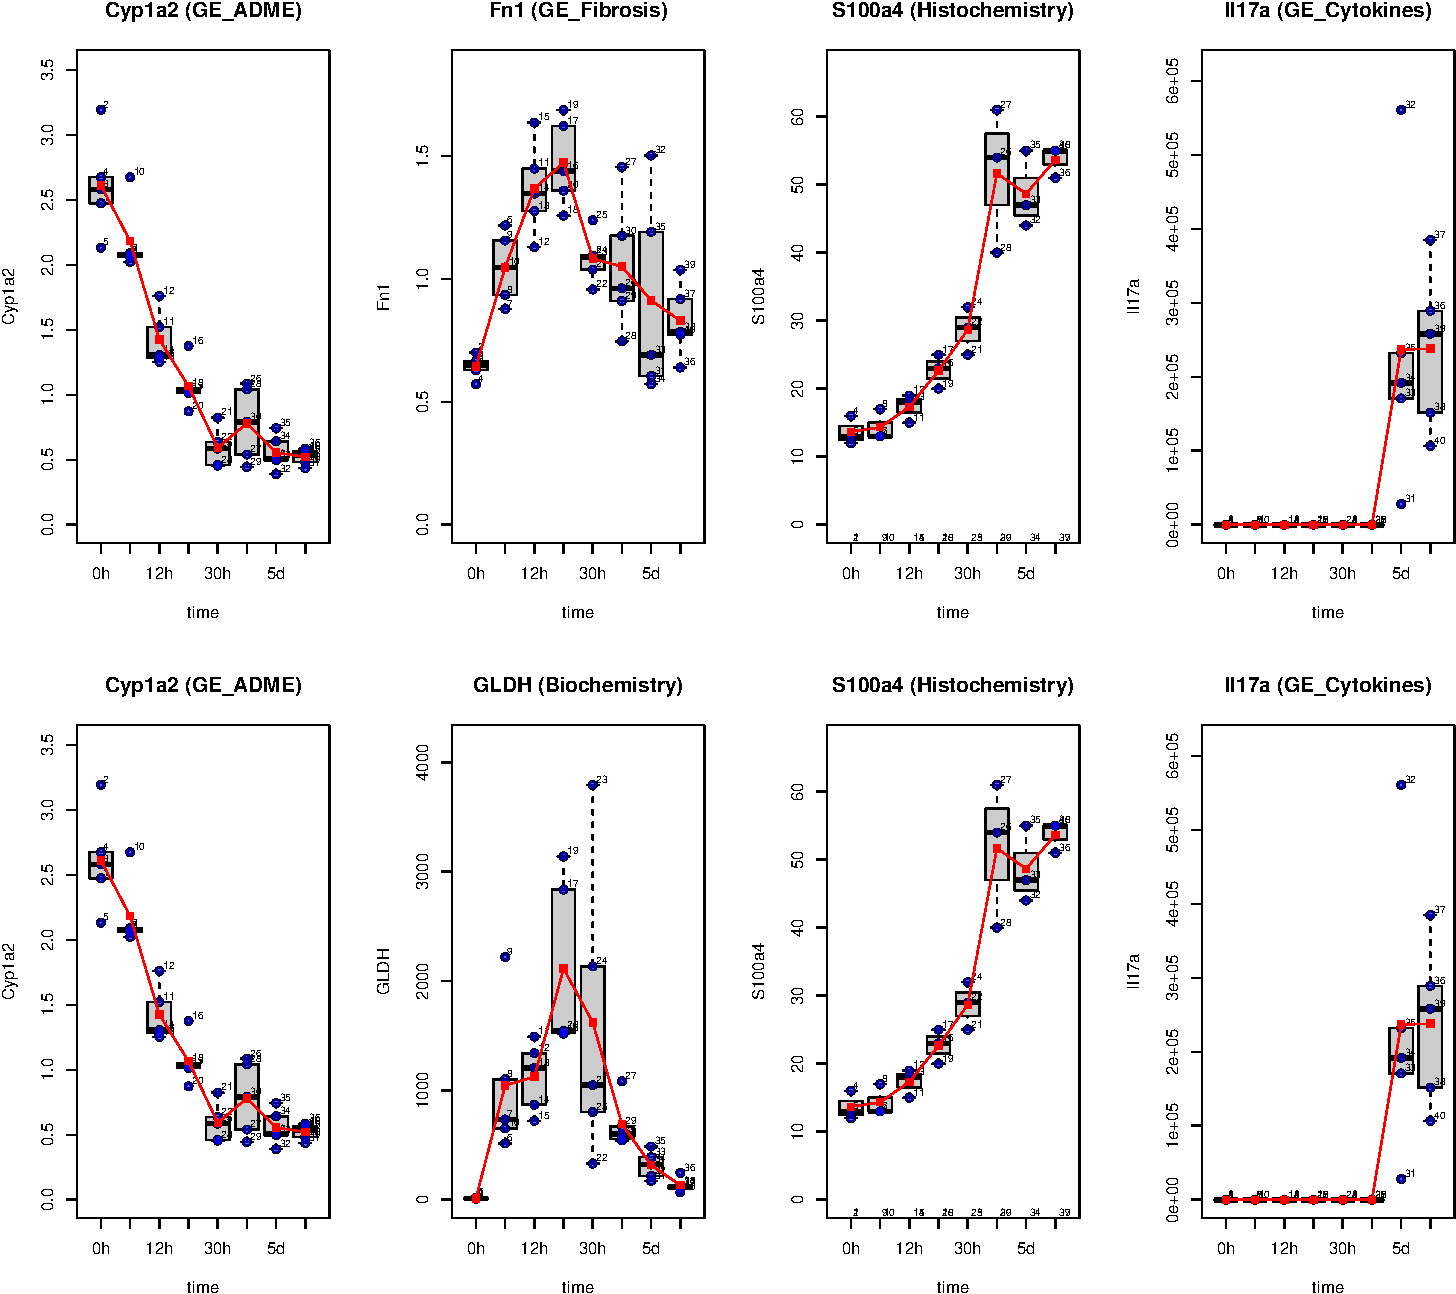
\includegraphics{Figs/plot_tree_all-1.pdf}

Figure: Best factor combination using all factors. Two alternative
solutions for the single factor combinations.

\begin{Shaded}
\begin{Highlighting}[]
\KeywordTok{plot_tree_representatives}\NormalTok{(gene.best)}
\end{Highlighting}
\end{Shaded}

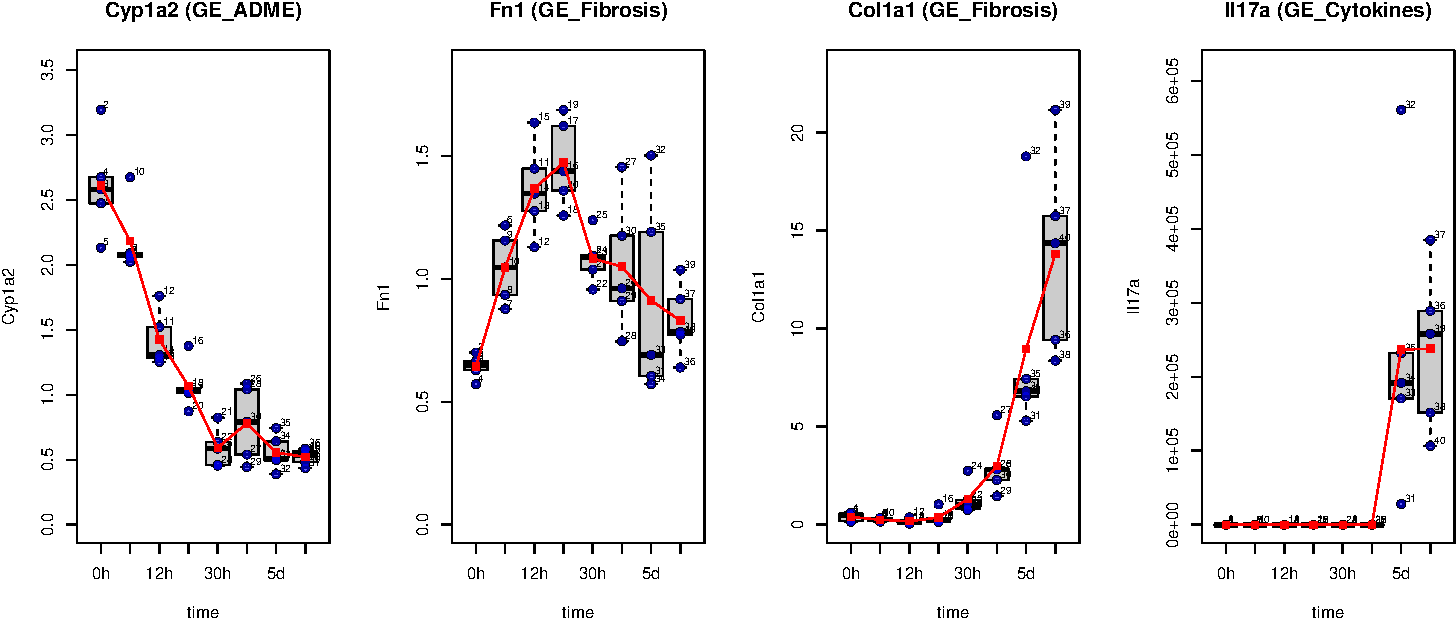
\includegraphics{Figs/plot_tree_gene-1.pdf}

Figure: Best factor combination using transcript factors.

\subsection{Prediction errors}\label{prediction-errors}

Plot the distance distributions of single and double representatives and
the best gene and representative trees.

\begin{Shaded}
\begin{Highlighting}[]
\CommentTok{# distance histogram}
\NormalTok{plot_tree_distance_dist <-}\StringTok{ }\NormalTok{function()\{}
  \NormalTok{breaks <-}\StringTok{ }\KeywordTok{seq}\NormalTok{(}\DataTypeTok{from=}\DecValTok{0}\NormalTok{, }\DataTypeTok{to=}\FloatTok{0.40}\NormalTok{, }\DataTypeTok{by=}\FloatTok{0.0125}\NormalTok{)}
  \KeywordTok{hist}\NormalTok{(dist.single, }\DataTypeTok{freq=}\OtherTok{FALSE}\NormalTok{, }\DataTypeTok{breaks=}\NormalTok{breaks,}
      \DataTypeTok{main=}\StringTok{"Prediction error"}\NormalTok{,}
      \DataTypeTok{xlab=}\StringTok{"RMSD(time.predicted, time.exp)"}\NormalTok{,}
      \DataTypeTok{col=}\KeywordTok{rgb}\NormalTok{(}\FloatTok{0.7}\NormalTok{,}\FloatTok{0.7}\NormalTok{,}\FloatTok{0.7}\NormalTok{, }\DecValTok{1}\NormalTok{),}
      \DataTypeTok{ylim=}\KeywordTok{c}\NormalTok{(}\DecValTok{0}\NormalTok{,}\DecValTok{15}\NormalTok{)}
  \NormalTok{)}
  \KeywordTok{hist}\NormalTok{(dist.double, }\DataTypeTok{freq=}\OtherTok{FALSE}\NormalTok{, }\DataTypeTok{breaks=}\NormalTok{breaks,}
       \DataTypeTok{col=}\KeywordTok{rgb}\NormalTok{(}\DecValTok{1}\NormalTok{,}\DecValTok{0}\NormalTok{,}\DecValTok{0}\NormalTok{, }\FloatTok{0.5}\NormalTok{), }\DataTypeTok{add=}\OtherTok{TRUE}\NormalTok{)}
  
  \KeywordTok{abline}\NormalTok{(}\DataTypeTok{v=}\NormalTok{dist.mean, }\DataTypeTok{col=}\KeywordTok{rgb}\NormalTok{(}\DecValTok{0}\NormalTok{,}\DecValTok{0}\NormalTok{,}\DecValTok{1}\NormalTok{, }\FloatTok{0.5}\NormalTok{), }\DataTypeTok{lwd=}\DecValTok{2}\NormalTok{)}
  \KeywordTok{abline}\NormalTok{(}\DataTypeTok{v=}\NormalTok{dist.rep.best, }\DataTypeTok{col=}\StringTok{"black"}\NormalTok{, }\DataTypeTok{lwd=}\DecValTok{2}\NormalTok{)}
  \KeywordTok{abline}\NormalTok{(}\DataTypeTok{v=}\NormalTok{dist.gene.best, }\DataTypeTok{col=}\StringTok{"grey"}\NormalTok{, }\DataTypeTok{lwd=}\DecValTok{2}\NormalTok{)}
  
  \KeywordTok{legend}\NormalTok{(}\StringTok{"topright"}\NormalTok{, }\DataTypeTok{legend=}\KeywordTok{c}\NormalTok{(}\StringTok{"single factor"}\NormalTok{, }\StringTok{"double factor"}\NormalTok{, }\StringTok{"mean cluster"}\NormalTok{), }
             \DataTypeTok{col=}\KeywordTok{c}\NormalTok{(}\KeywordTok{rgb}\NormalTok{(}\FloatTok{0.7}\NormalTok{, }\FloatTok{0.7}\NormalTok{, }\FloatTok{0.7}\NormalTok{, }\DecValTok{1}\NormalTok{),}\KeywordTok{rgb}\NormalTok{(}\DecValTok{1}\NormalTok{, }\DecValTok{0}\NormalTok{, }\DecValTok{0}\NormalTok{, }\FloatTok{0.5}\NormalTok{),}\KeywordTok{rgb}\NormalTok{(}\DecValTok{0}\NormalTok{, }\DecValTok{0}\NormalTok{, }\DecValTok{1}\NormalTok{, }\FloatTok{0.5}\NormalTok{)),}
             \DataTypeTok{bty=}\StringTok{"n"}\NormalTok{, }\DataTypeTok{cex=}\FloatTok{1.0}\NormalTok{, }\DataTypeTok{pch=}\DecValTok{15}\NormalTok{)}
\NormalTok{\}}
\CommentTok{# plot to file}
\KeywordTok{pdf}\NormalTok{(}\KeywordTok{file.path}\NormalTok{(resultsPath, }\StringTok{"decision_tree"}\NormalTok{, }\StringTok{"tree_distance_distribution.pdf"}\NormalTok{), }
    \DataTypeTok{width=}\DecValTok{10}\NormalTok{, }\DataTypeTok{height=}\DecValTok{6}\NormalTok{, }\DataTypeTok{pointsize=}\DecValTok{14}\NormalTok{)}
\KeywordTok{plot_tree_distance_dist}\NormalTok{()}
\KeywordTok{invisible}\NormalTok{(}\KeywordTok{dev.off}\NormalTok{())}
\end{Highlighting}
\end{Shaded}

\begin{Shaded}
\begin{Highlighting}[]
\KeywordTok{plot_tree_distance_dist}\NormalTok{()}
\end{Highlighting}
\end{Shaded}

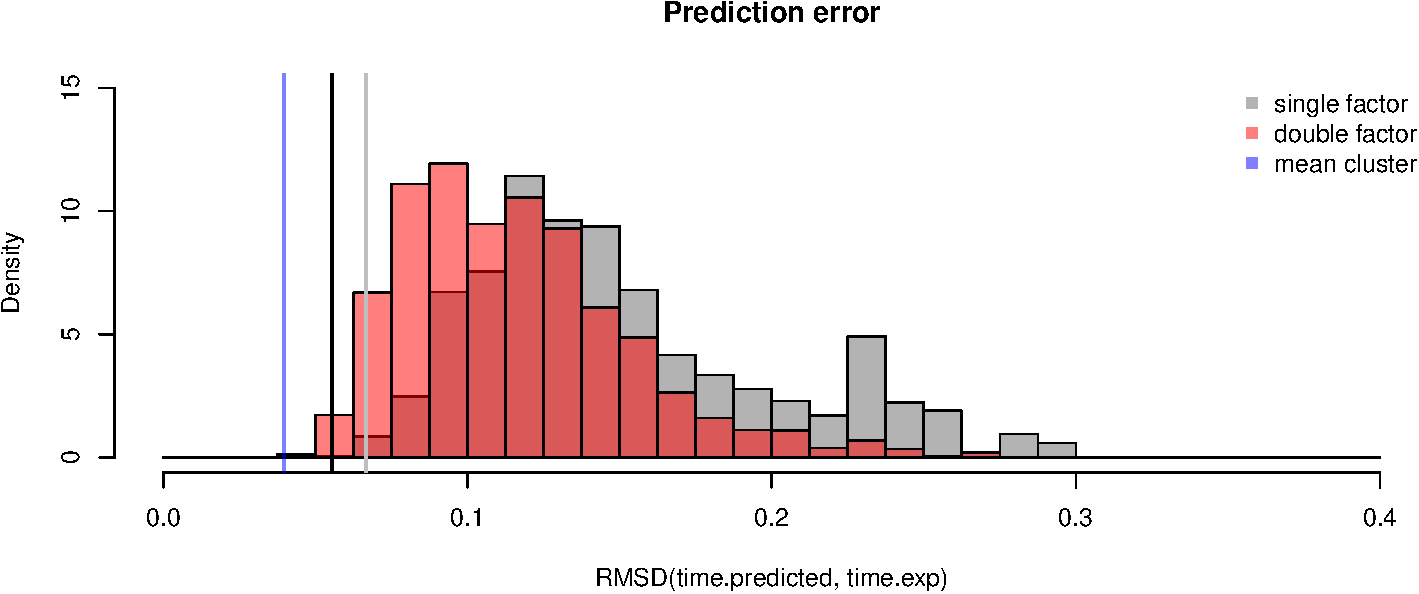
\includegraphics{Figs/plot_tree_distance-1.pdf}

Figure: Prediction error of regression tree. Distribution of distances
for single factor combinations, double factor combinations, mean cluster
data, best gene factor combination, and best all factor combination.
Adding additional factors to the prediction improves the predictions.

\subsection{Predictive performance}\label{predictive-performance}

Evaluation of the predictive performance of the regression trees by
analysing which time points are predicted in which time classes. I.e.
which experimental classes were predicted in which time classes of the
regression tree for the mean cluster data (trainings data), single
representative from each clusters and double representatives from each
cluster.

\begin{Shaded}
\begin{Highlighting}[]
\CommentTok{# Predicted classes of the regression tree}
\NormalTok{node_levels <-}\StringTok{ }\KeywordTok{levels}\NormalTok{(}\KeywordTok{as.factor}\NormalTok{(pred.mean))}
\NormalTok{node_classes <-}\StringTok{ }\KeywordTok{round}\NormalTok{(}\KeywordTok{as.numeric}\NormalTok{(node_levels), }\DataTypeTok{digits=}\DecValTok{1}\NormalTok{)}

\CommentTok{# Plot of the predicted classes with the decision tree}
\NormalTok{plot_predicted_classes <-}\StringTok{ }\NormalTok{function()\{}
  \CommentTok{# bar_colors <- brewer.pal(4, "Set3")}
  \NormalTok{bar_colors <-}\StringTok{ }\KeywordTok{c}\NormalTok{(}\KeywordTok{rgb}\NormalTok{(}\FloatTok{0.9}\NormalTok{,}\FloatTok{0.9}\NormalTok{,}\FloatTok{0.9}\NormalTok{), }
                  \KeywordTok{rgb}\NormalTok{(}\FloatTok{0.7}\NormalTok{,}\FloatTok{0.7}\NormalTok{,}\FloatTok{0.7}\NormalTok{),}
                  \KeywordTok{rgb}\NormalTok{(}\DecValTok{1}\NormalTok{,}\DecValTok{0}\NormalTok{,}\DecValTok{0}\NormalTok{, }\FloatTok{0.5}\NormalTok{),}
                  \KeywordTok{rgb}\NormalTok{(}\DecValTok{0}\NormalTok{,}\DecValTok{0}\NormalTok{,}\DecValTok{1}\NormalTok{, }\FloatTok{0.5}\NormalTok{))}
  \KeywordTok{par}\NormalTok{(}\DataTypeTok{mfrow=}\KeywordTok{c}\NormalTok{(}\DecValTok{2}\NormalTok{,}\DecValTok{4}\NormalTok{))}
  \NormalTok{for (k in }\DecValTok{1}\NormalTok{:Nt)\{}
    \CommentTok{# single factor predictions}
    \NormalTok{data <-}\StringTok{ }\KeywordTok{as.vector}\NormalTok{(pred.single[, ((}\DecValTok{1}\NormalTok{:Nr)+Nr*(k}\DecValTok{-1}\NormalTok{))])}
    \NormalTok{tab.single <-}\StringTok{ }\KeywordTok{table}\NormalTok{(}\KeywordTok{factor}\NormalTok{(data, }\DataTypeTok{levels=}\NormalTok{node_levels))/}\KeywordTok{length}\NormalTok{(data)}
    \CommentTok{# two factor predictions}
    \NormalTok{data <-}\StringTok{ }\KeywordTok{as.vector}\NormalTok{(pred.double[, ((}\DecValTok{1}\NormalTok{:Nr)+Nr*(k}\DecValTok{-1}\NormalTok{))])}
    \NormalTok{tab.double <-}\StringTok{ }\KeywordTok{table}\NormalTok{(}\KeywordTok{factor}\NormalTok{(data, }\DataTypeTok{levels=}\NormalTok{node_levels))/}\KeywordTok{length}\NormalTok{(data)}
    \CommentTok{# mean cluster predictions}
    \NormalTok{data <-}\StringTok{ }\KeywordTok{as.vector}\NormalTok{(pred.mean[((}\DecValTok{1}\NormalTok{:Nr)+Nr*(k}\DecValTok{-1}\NormalTok{))])}
    \NormalTok{tab.mean <-}\StringTok{ }\KeywordTok{table}\NormalTok{(}\KeywordTok{factor}\NormalTok{(data, }\DataTypeTok{levels=}\NormalTok{node_levels))/}\KeywordTok{length}\NormalTok{(data)}
    \CommentTok{# best single gene representative}
    \NormalTok{data <-}\StringTok{ }\KeywordTok{as.vector}\NormalTok{(pred.gene.best[((}\DecValTok{1}\NormalTok{:Nr)+Nr*(k}\DecValTok{-1}\NormalTok{))])}
    \NormalTok{tab.gene.best <-}\StringTok{ }\KeywordTok{table}\NormalTok{(}\KeywordTok{factor}\NormalTok{(data, }\DataTypeTok{levels=}\NormalTok{node_levels))/}\KeywordTok{length}\NormalTok{(data)}
    
    \CommentTok{# combined table}
    \NormalTok{tab <-}\StringTok{ }\KeywordTok{rbind}\NormalTok{(tab.single, tab.double, tab.gene.best, tab.mean)}
    \KeywordTok{colnames}\NormalTok{(tab) <-}\StringTok{ }\KeywordTok{round}\NormalTok{(}\KeywordTok{as.numeric}\NormalTok{(}\KeywordTok{colnames}\NormalTok{(tab)), }\DataTypeTok{digits=}\DecValTok{1}\NormalTok{)}
    
    \CommentTok{# create the bar plot}
    \NormalTok{name <-}\StringTok{ }\KeywordTok{sprintf}\NormalTok{(}\StringTok{"Time after BDL: %sh"}\NormalTok{, }\KeywordTok{levels}\NormalTok{(}\KeywordTok{as.factor}\NormalTok{(BDLsamples$time))[k])}
    \KeywordTok{barplot}\NormalTok{(tab, }\DataTypeTok{beside=}\OtherTok{TRUE}\NormalTok{,}
            \DataTypeTok{main=}\NormalTok{name, }
            \DataTypeTok{xlab=}\StringTok{"predicted time class [h]"}\NormalTok{, }\DataTypeTok{ylab=}\StringTok{"fraction of predictions"}\NormalTok{,}
            \DataTypeTok{ylim=}\KeywordTok{c}\NormalTok{(}\DecValTok{0}\NormalTok{,}\DecValTok{1}\NormalTok{), }\DataTypeTok{col=}\NormalTok{bar_colors) }
    \NormalTok{if (k==}\DecValTok{1}\NormalTok{)\{}
      \KeywordTok{legend}\NormalTok{(}\StringTok{"topright"}\NormalTok{, }\DataTypeTok{legend=}\KeywordTok{c}\NormalTok{(}\StringTok{"single factors"}\NormalTok{, }\StringTok{"double factors"}\NormalTok{, }
                                  \StringTok{"best single gene"}\NormalTok{, }\StringTok{"mean cluster"}\NormalTok{), }
             \DataTypeTok{col=}\NormalTok{bar_colors,}
             \DataTypeTok{bty=}\StringTok{"n"}\NormalTok{, }\DataTypeTok{cex=}\FloatTok{1.0}\NormalTok{, }\DataTypeTok{pch=}\DecValTok{15}\NormalTok{)}
    \NormalTok{\}}
  \NormalTok{\}}
  \KeywordTok{par}\NormalTok{(}\DataTypeTok{mfrow=}\KeywordTok{c}\NormalTok{(}\DecValTok{1}\NormalTok{,}\DecValTok{1}\NormalTok{))}
\NormalTok{\}}
\end{Highlighting}
\end{Shaded}

\begin{Shaded}
\begin{Highlighting}[]
\KeywordTok{plot_predicted_classes}\NormalTok{()}
\end{Highlighting}
\end{Shaded}

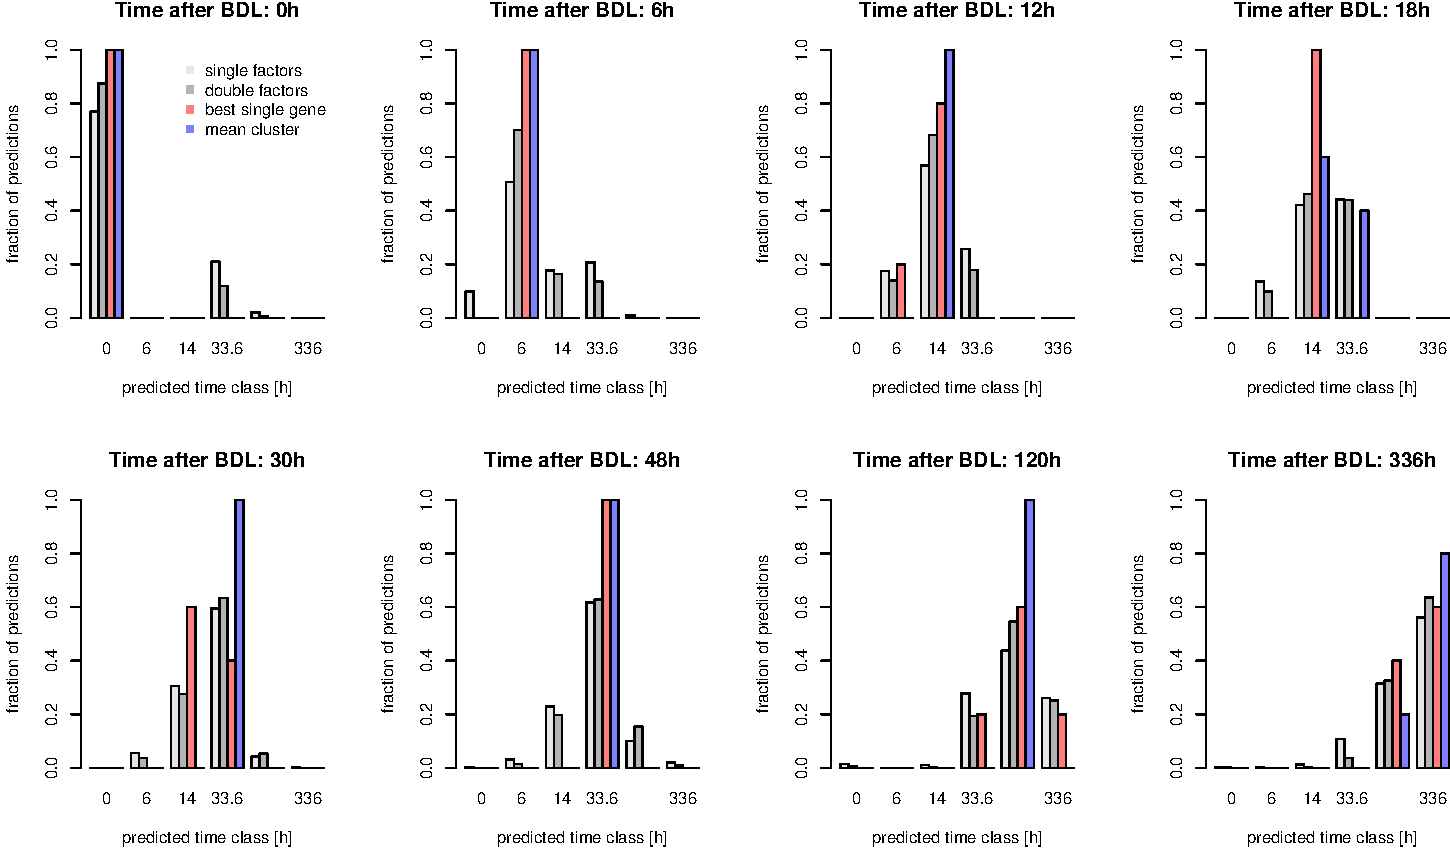
\includegraphics{Figs/plot_tree_bar1-1.pdf}

Figure: Prediction performance of regression tree.

\begin{Shaded}
\begin{Highlighting}[]
\CommentTok{# reverse bar plot}
\KeywordTok{library}\NormalTok{(plyr)}
\KeywordTok{library}\NormalTok{(reshape2)}

\CommentTok{# which experiments are predicted in which class}
\NormalTok{plot_predicted_classes2 <-}\StringTok{ }\NormalTok{function()\{}
  \NormalTok{bar_colors <-}\StringTok{ }\KeywordTok{c}\NormalTok{(}\KeywordTok{rgb}\NormalTok{(}\DecValTok{1}\NormalTok{,}\DecValTok{1}\NormalTok{,}\DecValTok{1}\NormalTok{), }
                  \KeywordTok{rgb}\NormalTok{(}\FloatTok{0.8}\NormalTok{,}\FloatTok{0.8}\NormalTok{,}\FloatTok{0.8}\NormalTok{),}
                  \KeywordTok{rgb}\NormalTok{(}\DecValTok{1}\NormalTok{,}\DecValTok{0}\NormalTok{,}\DecValTok{0}\NormalTok{, }\FloatTok{0.5}\NormalTok{),}
                  \KeywordTok{rgb}\NormalTok{(}\DecValTok{0}\NormalTok{,}\DecValTok{0}\NormalTok{,}\DecValTok{1}\NormalTok{, }\FloatTok{0.5}\NormalTok{))}
  \CommentTok{# single}
  \NormalTok{df <-}\StringTok{ }\KeywordTok{data.frame}\NormalTok{(}\DataTypeTok{exp=}\KeywordTok{rep}\NormalTok{(BDLsamples$time, Nsingle), }
                 \DataTypeTok{pre=}\KeywordTok{as.vector}\NormalTok{(}\KeywordTok{t}\NormalTok{(}\KeywordTok{round}\NormalTok{(pred.single, }\DataTypeTok{digits=}\DecValTok{1}\NormalTok{))) )}
  \NormalTok{tmp <-}\StringTok{ }\KeywordTok{count}\NormalTok{(df, }\KeywordTok{c}\NormalTok{(}\StringTok{"exp"}\NormalTok{, }\StringTok{"pre"}\NormalTok{))}
  \NormalTok{tab.single <-}\StringTok{ }\KeywordTok{acast}\NormalTok{(tmp, exp~pre, }\DataTypeTok{value.var=}\StringTok{"freq"}\NormalTok{, }\DataTypeTok{fill=}\DecValTok{0}\NormalTok{)}
  \CommentTok{# double}
  \NormalTok{df <-}\StringTok{ }\KeywordTok{data.frame}\NormalTok{(}\DataTypeTok{exp=}\KeywordTok{rep}\NormalTok{(BDLsamples$time, Ndouble), }
                 \DataTypeTok{pre=}\KeywordTok{as.vector}\NormalTok{(}\KeywordTok{t}\NormalTok{(}\KeywordTok{round}\NormalTok{(pred.double, }\DataTypeTok{digits=}\DecValTok{1}\NormalTok{))) )}
  \NormalTok{tmp <-}\StringTok{ }\KeywordTok{count}\NormalTok{(df, }\KeywordTok{c}\NormalTok{(}\StringTok{"exp"}\NormalTok{, }\StringTok{"pre"}\NormalTok{))}
  \NormalTok{tab.double <-}\StringTok{ }\KeywordTok{acast}\NormalTok{(tmp, exp~pre, }\DataTypeTok{value.var=}\StringTok{"freq"}\NormalTok{, }\DataTypeTok{fill=}\DecValTok{0}\NormalTok{)}
  \CommentTok{# best gene}
  \NormalTok{df <-}\StringTok{ }\KeywordTok{data.frame}\NormalTok{(}\DataTypeTok{exp=}\KeywordTok{rep}\NormalTok{(BDLsamples$time, }\DecValTok{1}\NormalTok{), }
                 \DataTypeTok{pre=}\KeywordTok{as.vector}\NormalTok{(}\KeywordTok{t}\NormalTok{(}\KeywordTok{round}\NormalTok{(pred.gene.best, }\DataTypeTok{digits=}\DecValTok{1}\NormalTok{))) )}
  \NormalTok{tmp <-}\StringTok{ }\KeywordTok{count}\NormalTok{(df, }\KeywordTok{c}\NormalTok{(}\StringTok{"exp"}\NormalTok{, }\StringTok{"pre"}\NormalTok{))}
  \NormalTok{tab.gene.best <-}\StringTok{ }\KeywordTok{acast}\NormalTok{(tmp, exp~pre, }\DataTypeTok{value.var=}\StringTok{"freq"}\NormalTok{, }\DataTypeTok{fill=}\DecValTok{0}\NormalTok{)}
  \CommentTok{# mean cluster}
  \NormalTok{df <-}\StringTok{ }\KeywordTok{data.frame}\NormalTok{(}\DataTypeTok{exp=}\KeywordTok{rep}\NormalTok{(BDLsamples$time, }\DecValTok{1}\NormalTok{), }
                 \DataTypeTok{pre=}\KeywordTok{as.vector}\NormalTok{(}\KeywordTok{t}\NormalTok{(}\KeywordTok{round}\NormalTok{(pred.mean, }\DataTypeTok{digits=}\DecValTok{1}\NormalTok{))) )}
  \NormalTok{tmp <-}\StringTok{ }\KeywordTok{count}\NormalTok{(df, }\KeywordTok{c}\NormalTok{(}\StringTok{"exp"}\NormalTok{, }\StringTok{"pre"}\NormalTok{))}
  \NormalTok{tab.mean <-}\StringTok{ }\KeywordTok{acast}\NormalTok{(tmp, exp~pre, }\DataTypeTok{value.var=}\StringTok{"freq"}\NormalTok{, }\DataTypeTok{fill=}\DecValTok{0}\NormalTok{)  }

  \KeywordTok{par}\NormalTok{(}\DataTypeTok{mfrow=}\KeywordTok{c}\NormalTok{(}\DecValTok{2}\NormalTok{,}\DecValTok{3}\NormalTok{))  }
  \NormalTok{for (k in }\DecValTok{1}\NormalTok{:}\KeywordTok{length}\NormalTok{(node_classes))\{}
    \CommentTok{# combined table (normalized within each class)}
    \NormalTok{tab <-}\StringTok{ }\KeywordTok{rbind}\NormalTok{(tab.single[,k]/}\KeywordTok{sum}\NormalTok{(tab.single[,k]),}
                 \NormalTok{tab.double[,k]/}\KeywordTok{sum}\NormalTok{(tab.double[,k]), }
                 \NormalTok{tab.gene.best[,k]/}\KeywordTok{sum}\NormalTok{(tab.gene.best[,k]),}
                 \NormalTok{tab.mean[,k]/}\KeywordTok{sum}\NormalTok{(tab.mean[,k]))}

    \CommentTok{# create the bar plot}
    \NormalTok{name <-}\StringTok{ }\KeywordTok{sprintf}\NormalTok{(}\StringTok{"Predicted: %sh"}\NormalTok{, node_classes[k])}
    \KeywordTok{barplot}\NormalTok{(tab, }\DataTypeTok{beside=}\OtherTok{TRUE}\NormalTok{,}
            \DataTypeTok{main=}\NormalTok{name, }
            \DataTypeTok{xlab=}\StringTok{"time after BDL [h]"}\NormalTok{, }\DataTypeTok{ylab=}\StringTok{"fraction"}\NormalTok{,}
            \DataTypeTok{ylim=}\KeywordTok{c}\NormalTok{(}\DecValTok{0}\NormalTok{,}\DecValTok{1}\NormalTok{), }\DataTypeTok{col=}\NormalTok{bar_colors) }
    \NormalTok{if (k==}\DecValTok{1}\NormalTok{)\{}
      \KeywordTok{legend}\NormalTok{(}\StringTok{"topright"}\NormalTok{, }\DataTypeTok{legend=}\KeywordTok{c}\NormalTok{(}\StringTok{"single factors"}\NormalTok{, }\StringTok{"double factors"}\NormalTok{, }
                                  \StringTok{"best gene"}\NormalTok{, }\StringTok{"mean cluster"}\NormalTok{), }
             \DataTypeTok{col=}\NormalTok{bar_colors,}
             \DataTypeTok{bty=}\StringTok{"n"}\NormalTok{, }\DataTypeTok{cex=}\FloatTok{1.0}\NormalTok{, }\DataTypeTok{pch=}\DecValTok{15}\NormalTok{)}
    \NormalTok{\}}
  \NormalTok{\}}
  \KeywordTok{par}\NormalTok{(}\DataTypeTok{mfrow=}\KeywordTok{c}\NormalTok{(}\DecValTok{1}\NormalTok{,}\DecValTok{1}\NormalTok{))}
\NormalTok{\}}

\CommentTok{# barplot to file}
\KeywordTok{pdf}\NormalTok{(}\KeywordTok{file.path}\NormalTok{(resultsPath, }\StringTok{"decision_tree"}\NormalTok{, }\StringTok{"predicted_classes2.pdf"}\NormalTok{), }
    \DataTypeTok{width=}\DecValTok{12}\NormalTok{, }\DataTypeTok{height=}\FloatTok{7.5}\NormalTok{, }\DataTypeTok{pointsize=}\DecValTok{14}\NormalTok{)}
\KeywordTok{plot_predicted_classes2}\NormalTok{()}
\KeywordTok{invisible}\NormalTok{(}\KeywordTok{dev.off}\NormalTok{())}
\end{Highlighting}
\end{Shaded}

\begin{Shaded}
\begin{Highlighting}[]
\KeywordTok{plot_predicted_classes2}\NormalTok{()}
\end{Highlighting}
\end{Shaded}

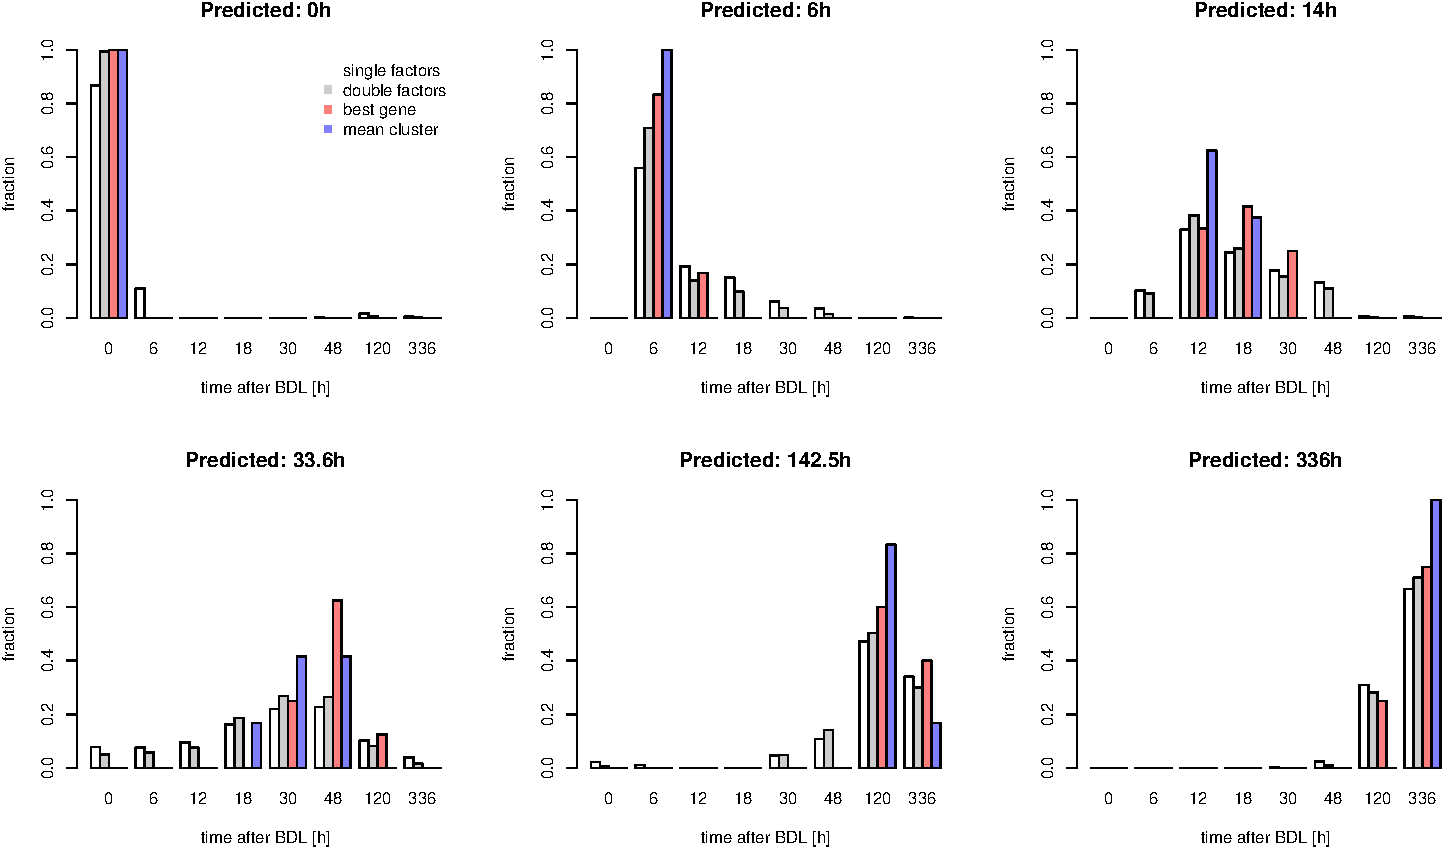
\includegraphics{Figs/plot_tree_bar2-1.pdf}

Figure: Prediction performance of regression tree.

\end{document}
